\cotefile{8}
\scanpage{79}
Si p.ex. \deleted{\unsure{$n=p$} \illegible{3}} \inserted{si $\Lambda$ est un corps, (p.ex. $\Lambda=\mathbb F_p$\deleted{\unsure{$\mathbf Z$}})}, le $\mathbb L$ sur le dernier $\otimes$ est inutile, on peut écrire
\[
(1.4')\qquad \ell^{\unsure{G|C}}_{\bullet}\simeq (M\overset{\mathbb L}{\otimes}_{\mathbb Z}\mathbb F_p)\otimes_{\mathbb F_p}\underline{\mathrm O}_S.
\]
1.5. \deleted{\unsure{2.}} Supposons qu'on ait un revêtement \deleted{\unsure{étale}} principal $S'$ de $S$ de groupe \deleted{\unsure{ordinaire}} $\pi$ discret ou profini, et que $M$ provienne par descente d'une \deleted{\unsure{représentation}} représentation de $\pi$ dans un groupe abélien $M_0$ (qu'on suppose continue pour $\pi$ profini); p.ex. si $M$ est isotrivial (p.ex. à fibres de \unsure{V.|type} fini et $S$ \deleted{\unsure{connexe}} normal) et si $S$ connexe, alors on sera dans la situation dite, avec $S'$ le rev. universel de $S$....

On a donc un hom. de topos
\diagram{\begin{tikzcd}[ampersand replacement=\&]
(1.6)\qquad \underset{\substack{(\text{top. ét.,}\\\text{\unsure{ou|---} fpqc}\\\text{\unsure{ou|---} fppf})}}{(S\deleted{\unsure{\underline{\mathrm O}_S}})} \arrow[r,"f"] \& (B_\pi\deleted{\unsure{\mathbb Z}})
\end{tikzcd}}
avec
\[
(1.7)\qquad M=f^{\deleted{\unsure{*}}\inserted{-1}}(M_0).
\]
On aura alors, si on annèle $S$ et $B_\pi$ par l'anneau constant $\Lambda$, et envisage $f$ en conséquence
\[
\deleted{\unsure{(1.7)}}\qquad M\overset{\mathbb L}{\otimes}_{\mathbb Z}\Lambda=f^*(M_0\overset{\mathbb L}{\otimes}_{\mathbb Z}\Lambda)
\]
et par suite on peut écrire
\[
(1.8)\qquad \ell^{\unsure{G|C}}_{\bullet}\simeq f^*(M_0\overset{\mathbb L}{\otimes}_{\mathbb Z}\Lambda)\overset{\mathbb L}{\otimes}_{\Lambda}\underline{\mathrm O}_S,
\]
où le $\mathbb L$ sur $\otimes_\Lambda$ est inutile si $\Lambda$ est un corps....
\mspage{78}

\scanpage{80}
2. Notons que \deleted{si $\underline{\mathrm O}_S$ est de car. \unsure{$p$}} l'on tire de (1.3)
\[
(2.1)\qquad\left\{\begin{aligned}
\omega_G&=\underline M\otimes_{\mathbb Z}\underline{\mathrm O}_S\\
\underline n_G&=\underline{\operatorname{Tor}}_1^{\mathbb Z}(M,\underline{\mathrm O}_S)
\end{aligned}\right.
\]
ce qui s'écrit, si $S$ est de car. $p>0$
\[
\unsure{(2.1)|(2.2)}\qquad\left\{\begin{aligned}
\omega_G&=(M\otimes_{\mathbb Z}\mathbb F_p)\otimes_{\mathbb F_p}\underline{\mathrm O}_S=M_p\otimes_{\mathbb F_p}\underline{\mathrm O}_S\\
\underline n_G&\simeq {}_pM\otimes_{\mathbb F_p}\underline{\mathrm O}_S
\end{aligned}\right.
\]
et si $M$ est annulé par $p$, i.e. $G$ annulé par $p$ cela devient
\[
(2.2')\qquad \omega_G\simeq M\otimes_{\mathbb F_p}\underline{\mathrm O}_S,\qquad \underline n_G\simeq M\otimes_{\mathbb F_p}\underline{\mathrm O}_S.
\]
On a d'autre part une classe canonique
\[
\unsure{\xi|\zeta}\in\operatorname{Ext}^{2}_{\underline{\mathrm O}_S}(M\otimes_{\mathbb Z}\underline{\mathrm O}_S,\underline{\operatorname{Tor}}_1^{\mathbb Z}(M,\underline{\mathrm O}_S))
\]
qu'on peut interpréter, en présence d'un $\Lambda$, comme provenant d'un
\[
\unsure{\xi|\zeta}_\Lambda\in\operatorname{Ext}^{2}_{\Lambda}(M\otimes_{\mathbb Z}\Lambda,\operatorname{Tor}_1^{\mathbb Z}(M,\Lambda));
\]
Supposons p.ex. que $\Lambda=\mathbb Z/n\mathbb Z$, et que \deleted{$M\unsure{\otimes}$}\inserted{$M$} soit un $\Lambda$-module loc. libre de t.f. Alors il en est de $=$ de $M\otimes_{\mathbb Z}\Lambda\simeq M$ et de $\operatorname{Tor}_1^{\mathbb Z}(M,\Lambda)\simeq{}_nM\simeq M$, et
\[
\unsure{\xi|\zeta}_\Lambda\in\mathrm H^2(S,\operatorname{End}(M)),
\]
et \deleted{si \unsure{$\xi\in$} $\underline{\mathrm O}_S$ est plat sur $\Lambda$ (p.ex. $n=p$)}
\[
\unsure{\xi|\zeta}\in\mathrm H^2(S,\operatorname{End}(E))\qquad(E=M\otimes_\Lambda\underline{\mathrm O}_S)
\]
et $\unsure{\xi|\zeta}$ est déduit de $\unsure{\xi|\zeta}_\Lambda$ par l'hom. can.
\mspage{79}

\scanpage{81}
\diagram{\begin{tikzcd}[ampersand replacement=\&,column sep=small]
\mathrm H^{\unsure{*|2}}(S,\operatorname{End}(M)) \arrow[r,dash] \& \mathrm H^{\unsure{*|2}}(S,\operatorname{End}(M)\otimes_\Lambda\underline{\mathrm O}_S)\simeq\mathrm H^2(S,\operatorname{End}(E))
\end{tikzcd}}
Enfin, sous les conditions de 1.5, $M_0$ étant aussi plat sur $\Lambda$, on aura que $\unsure{\xi|\zeta}_\Lambda$ est l'image d'un élément
\[
\unsure{\xi|\zeta}_0\in\mathrm H^2(B_\pi,\operatorname{End}(M_0)).
\]
(NB Pour calculer $\unsure{\xi|\zeta}_0$, par fonctorialité en $\pi$, on est ramené aussitôt au cas ``universel'' $\pi=\operatorname{Aut}(M_0)$, et on peut évidemment supposer $M_0=\Lambda^d=(\mathbb Z/n\mathbb Z)^d$, donc $\pi=\operatorname{GL}(d,\mathbb Z/n\mathbb Z)$ ....) D'après \uline{Illusie}, c'est l'obstruction à remonter la représentation de $\pi$ dans $M_0$ en une représentation dans un module libre sur $\mathbb Z/\unsure{p^2|n^2}\mathbb Z$.

\inserted{Lorsque $n=p$ (premier),} Elle est évidemment nulle si $M_0$ est de rang $\leq1$, mais sans doute pas nulle si $M_0$ de rang $d\geq2$, dans le cas universel $\pi=\operatorname{GL}(d,\mathbb F_p)$.

Notons que si le rev. $S'$ de $S$ est le rev. universel, alors
\diagram{\begin{tikzcd}[ampersand replacement=\&]
\mathrm H^2(B_\pi,-) \arrow[r] \& \mathrm H^2(S,-)
\end{tikzcd}}
est \uline{injectif}, donc on trouvera un élément non nul \deleted{dans} $\unsure{\xi|\zeta}_\Lambda\in\mathrm H^2(S,\operatorname{End}(M))$.
\mspage{80}

\cotefile{9}
\scanpage{1}
\figure{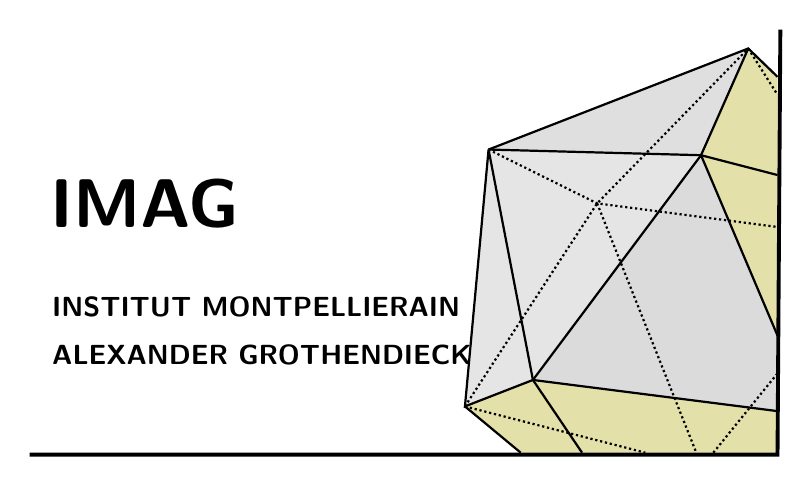
\begin{tikzpicture}[x=.012cm,y=-.012cm,line width=.8pt]
\node[anchor=west,font=\sffamily\bfseries\Huge] at (20,195) {IMAG};
\node[anchor=west,font=\sffamily\bfseries] at (22,305) {INSTITUT MONTPELLIERAIN};
\node[anchor=west,font=\sffamily\bfseries] at (22,355) {ALEXANDER GROTHENDIECK};
\fill[gray!25] (495,138)--(770,31)--(720,144)--cycle;
\fill[gray!20] (495,138)--(720,144)--(542,382)--(470,410)--cycle;
\fill[gray!28] (720,144)--(801,335)--(801,415)--(542,382)--cycle;
\fill[olive!25] (770,31)--(801,61)--(801,335)--(720,144)--cycle;
\fill[olive!25] (470,410)--(542,382)--(801,415)--(801,459)--(529,459)--cycle;
\draw (495,138)--(770,31)--(801,61);
\draw (495,138)--(720,144)--(770,31);
\draw (720,144)--(801,165);
\draw (495,138)--(470,410)--(542,382)--(495,138);
\draw (542,382)--(720,144)--(801,335);
\draw (470,410)--(529,459);
\draw (542,382)--(594,459);
\draw (542,382)--(801,415);
\draw[densely dotted] (495,138)--(610,195)--(801,220);
\draw[densely dotted] (470,410)--(610,195)--(770,31);
\draw[densely dotted] (610,195)--(715,459);
\draw[densely dotted] (470,410)--(661,459);
\draw[densely dotted] (733,459)--(801,375);
\draw[densely dotted] (770,31)--(801,80);
\draw[line width=1.4pt] (9,461)--(801,461)--(804,11);
\end{tikzpicture}}

\scanpage{2}
\uline{Dualité} des modules de Dieudonné de groupes de B. T. duaux l'un de l'autre ....

Le module de Dieudonné réduit
\[
M\otimes_W k
\]
\margin{\unsure{7}}
\mspage{1}

\scanpage{3}
$k$ corps de car $p>0$

$G$ grp $p$-divisible, $G^*$ dual
\[
g=\dim G,\quad g^*=\dim G^*
\]
$\widetilde G$ grp \unsure{enveloppant}
\diagram{\begin{tikzcd}[ampersand replacement=\&]
0\arrow[r]\&\underline V(t_{G^*})\arrow[r]\&\widetilde G\arrow[r]\&G\arrow[r]\&0
\end{tikzcd}}
\diagram{\begin{tikzcd}[ampersand replacement=\&,column sep=small,row sep=large]
0\arrow[r]\&\underset{\omega_G=}{t_G^\vee}\arrow[r]\&H(G)\arrow[r]\arrow[d,shift right,"H(V)=V_0"']\&t_{G^*}\arrow[r]\&0\\
0\arrow[r]\&\underset{\omega_G^{(p)}=}{t_G^{\vee(p)}}\arrow[r]\&H(G)^{(p)}\arrow[r]\arrow[u,shift right,"H(F)=F_0"']\&t_{G^*}^{(p)}\arrow[r]\&0\\
\&\text{dim }g\&\text{dim }g+g^*\&\text{dim }g^*
\end{tikzcd}\quad\vrule height 4cm depth 0cm\quad
\begin{tikzcd}[ampersand replacement=\&,column sep=small,row sep=large]
\text{duales} \& \& \& \& \\
0\arrow[r]\&\underset{\omega_{G^*}=}{t_{G^*}^\vee}\arrow[r]\&t_{\widetilde G}\arrow[r]\arrow[d,shift right,"V_0"']\&t_G\arrow[r]\&0\\
0\arrow[r]\&\underset{\omega_{G^*}^{(p)}=}{t_{G^*}^{\vee(p)}}\arrow[r]\&t_{\widetilde G}^{(p)}\arrow[r]\arrow[u,shift right,"F_0"']\&t_G^{(p)}\arrow[r]\&0
\end{tikzcd}}
\[
[\ \uline{\text{NB}}\quad H(G)=t_{\unsure{\widetilde{G^*}|G^*}}\deleted{\unsure{\vee}}\ ]
\]
\textcircled{1} \unsure{suites sont} pour $t_{\widetilde G}$ et $t_{\widetilde{G^*}}$ transposées l'une de l'autre pour un accouplement canonique fonctoriel, \deleted{\unsure{avec}} pour lequel $F_0$ et $V_0$ (si on est en car $p$) s'interchangent.

\textcircled{2} Dans la suite exacte de gauche, on a
\[
\begin{aligned}
\operatorname{Ker}F_0&=\operatorname{Im}V_0=t_G^{\vee(p)}=\omega_G^{(p)}\\
\operatorname{Ker}V_0&=\operatorname{Im}F_0=\text{\unsure{ce que ça peut} (\unsure{innovation intéressante})}
\end{aligned}
\]
\textcircled{3} $F_0$ et $V_0$ opérant sur $H(G)$ définissent le module de Dieudonné \deleted{de \unsure{$G$}} réduit mod $p$.

\margin{?}
\textcircled{4} La composée
\diagram{\begin{tikzcd}[ampersand replacement=\&]
t_{G^*}^{(p)}\arrow[r,"F_0"]\&H(G)\arrow[r,dash]\&t_{G^*}
\end{tikzcd}}
\deleted{\unsure{la multiplication}\ \illegible{2}}
\margin{correspond : la puissance $p$-ième dans \unsure{l'algèbre} [et correspond : Frobenius dans $H^{\unsure{2|1}}(G,\mathbf G_a)$]\quad $H(G)=t_{\widetilde{G^*}}$}

\uline{Corollaire}
\[
\begin{array}{rcl}
G\text{ purement infinitésimal}&\Longleftrightarrow&F_0\text{ nilpotent}\qquad\text{i.e. }G\text{ sans tore}\\
G^*\text{ purement infinitésimal}&\Longleftrightarrow&V_0\text{ nilpotent}\\[-2pt]
\text{i.e. }G\text{ sans composante}\ \text{toroïdale}&&\\
G\text{ et }G^*\text{ purement infinitésimaux}&\Longleftrightarrow&F_0\text{ et }V_0\text{ nilpotents}
\end{array}
\]
\mspage{2}

\scanpage{4}
\uline{UNIVERSITÀ DI PISA}\hfill Tel. 24.550

ISTITUTO MATEMATICO ``LEONIDA TONELLI''
\figure{\begin{tikzpicture}[x=1cm,y=1cm]
\draw (-1,0)--(-.1,0);\fill (-.08,-.025) rectangle (.08,.025);\draw (.1,0)--(1,0);
\end{tikzpicture}}
\figure{
\begin{tikzpicture}[scale=.25]
\foreach \y in {0,8,84} {
\draw[gray!25] (0,-\y)--(3,-\y)--(3,1.5-\y)--(2.4,1.7-\y)--(2.4,2.8-\y)--(1.5,4-\y)--(.6,2.8-\y)--(.6,1.7-\y)--(0,1.5-\y)--cycle;
\draw[gray!25] (.6,2.8-\y)--(2.4,2.8-\y) (.6,2.4-\y)--(2.4,2.4-\y) (1.2,-\y)--(1.2,1.2-\y)--(1.8,1.2-\y)--(1.8,-\y);
}
\foreach \y in {16,20,...,80} {
\draw[gray!20] (1,-\y) to[out=70,in=-100] (1.8,3-\y) to[out=-30,in=100] (2.4,-\y) to[out=-120,in=80] (1.4,-3-\y) to[out=150,in=-90] (1,-\y);
\draw[gray!20] (.8,-\y)--(2.5,-.5-\y);
}
\end{tikzpicture}}
\mspage{3}

\scanpage{5}
\[
\langle x,y\rangle=\varphi_n(xy)\qquad \varphi_n:A_n\mathbin{-}W_n
\]
a) $\varphi_n$ est \deleted{\unsure{bilin.}} linéaire : \uline{gauche et à droite} en $W_n$
\[
\boxed{\begin{gathered}\varphi_n(1)=1\\\varphi_n(F^i)=0,\quad\varphi_n(V^i)=0\\(i\geq1)\end{gathered}}\qquad \exists!
\]
b) $\varphi_n(Fz)=\deleted{\unsure{\pi}}\varphi_n(zF)^\pi$

\margin{$\varphi_n$}

c) $\varphi_n(zV)=\deleted{\unsure{\pi}}\varphi_n(Vz)^\pi$

\figure{\begin{tikzpicture}\draw (0,0)--(2,0);\end{tikzpicture}}
d) Les $\varphi_n$ se recollent (\unsure{$\varphi_n$ compatibles})
\[
\varphi_n(\underbrace{\unsure{a}+\sum_1^{\unsure{\infty}}\lambda_i F^i+\sum_1^{\unsure{\infty}}\deleted{\unsure{\mu_i}}V^i\mu_i}_{z})=
\]
\[
\deleted{\unsure{\varphi_n(1)=a}}\qquad
\deleted{\varphi_n(F\unsure{\sum_0\lambda_iF^i})=\unsure{\varphi_n(z)=a}}
\]
\[
\deleted{F^iV^i\longmapsto0}
\]
\[
\deleted{\varphi_n(\underbrace{\sum_{\unsure{0\leq i,j\leq n}}\unsure{a_{ij}|\lambda_{ij}}F^iV^j}_{z})=\lambda_{00}}
\]
\[
\deleted{\begin{gathered}\varphi_n(Fz)=p\unsure{\mu_1}\\\varphi_n(zF)=\end{gathered}}
\qquad \varphi_n(z)=a
\]
\[
\varphi_n(\lambda z)=\lambda\varphi_n(z)\quad\text{OK}
\]
\[
\varphi_n(z\lambda)=\varphi_n\left(\sum\lambda_{ij}\lambda^{\pi^{i-j}}F^iV^j\right)=\varphi_n(z)\lambda\qquad\text{OK.}
\]
\[
\deleted{\varphi_n(Fz)=\varphi_n\left(\sum\lambda_{ij}^{\pi}F^{i+1}V^j\right)=\varphi_n\unsure{(z)^\pi}\quad/\quad\varphi_n(zF)=\varphi_n\left(\sum\lambda_{ij}F^{i+1}V^j\right)}
\]
\[
\varphi_n(Fz)=\varphi_n(zF)=
\]
\mspage{4}

\scanpage{6}
\uline{UNIVERSITÀ DI PISA}

ISTITUTO MATEMATICO ``LEONIDA TONELLI''
\figure{\begin{tikzpicture}\draw (-1,0)--(-.1,0);\fill (-.08,-.025) rectangle (.08,.025);\draw (.1,0)--(1,0);\end{tikzpicture}}
\figure{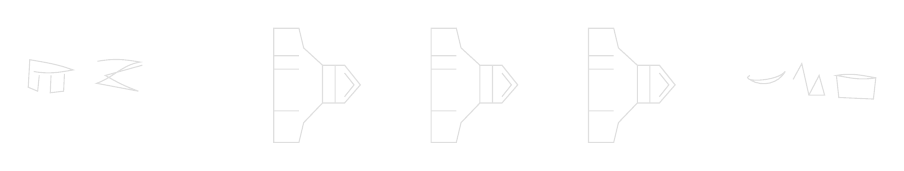
\begin{tikzpicture}[x=.01cm,y=-.01cm,line width=.4pt,draw=gray!25]
\foreach \x in {320,520,720} {
\draw (\x,0)--(\x,-90)--(\x+32,-90)--(\x+38,-65)--(\x+62,-43)--(\x+90,-43)--(\x+110,-18)--(\x+90,5)--(\x+62,5)--(\x+38,30)--(\x+32,55)--(\x,55)--cycle;
\draw (\x,-55)--(\x+32,-55) (\x,-38)--(\x+32,-38) (\x,15)--(\x+32,15) (\x+62,-43)--(\x+62,5) (\x+78,-43)--(\x+78,5) (\x+90,-33)--(\x+102,-18)--(\x+90,-3);
}
\draw (15,-35) to[out=-10,in=-170] (65,-37) to[out=160,in=-10] (10,-50)--(8,-15)--(20,-10)--(22,-30);
\draw (37,-30)--(36,-8)--(53,-10)--(54,-32);
\draw (96,-48) to[out=10,in=170] (150,-47) to[out=190,in=20] (95,-20)--(148,-10) to[out=160,in=-30] (106,-30)--(153,-43);
\draw (925,-30) to[out=-150,in=-130] (970,-35) to[out=-120,in=-30] (926,-24);
\draw (980,-25)--(991,-45)--(1000,-5)--(1020,-5)--(1013,-30)--(1000,-5);
\draw (1035,-30)--(1038,-2)--(1082,0)--(1085,-27) to[out=-170,in=-10] (1035,-30) to[out=10,in=170] (1085,-27);
\end{tikzpicture}}
\unsure{Arrive verci|Arrive derci}

\figure{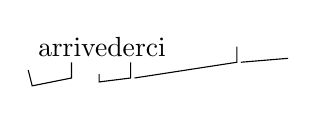
\begin{tikzpicture}[x=1cm,y=1cm]
\node[anchor=west] at (0,.4) {arrivederci};
\draw (0,.1)--(.05,-.1)--(.55,0)--(.55,.2);
\draw (.9,.05)--(.9,-.05)--(1.3,0)--(1.3,.2);
\draw (1.35,0)--(2.65,.2)--(2.65,.4);
\draw (2.7,.2)--(3.3,.25);
\end{tikzpicture}}
\[
\left[\begin{array}{l}
\text{buon giorno}\\
\text{\unsure{buona} sera}\\
\text{buona notte}\\
\text{per favore}\\
\text{mangare}\\
\text{\unsure{collazione|colazione}}
\end{array}\right.
\]
\figure{\begin{tikzpicture}[x=.01cm,y=-.01cm,line width=.7pt]
\node[rotate=90,anchor=west] at (90,-30) {Corso Italia};
\node[rotate=45,anchor=west] at (122,-140) {\unsure{Pizzeria}};
\draw (100,0)--(102,76)--(0,84);
\draw (155,0)--(158,73)--(370,72);
\draw (15,145)--(100,142);
\draw (165,132)--(320,132);
\draw (110,155)--(112,353)--(103,350);
\draw (160,162)--(158,340)--(340,346);
\draw (8,343)--(96,341);
\draw (0,400)--(95,398);
\draw (155,400)--(350,400)--(355,435)--(435,433)--(437,407)--(370,399);
\node at (398,415) {$\unsure{v}$};
\draw (112,400)--(120,510)--(126,504);
\draw (118,416)--(118,596);
\draw[->] (183,400)--(181,571);
\draw (215,460) .. controls (230,445) and (228,585) .. (210,600) .. controls (250,610) and (250,740) .. (212,768) .. controls (250,785) and (248,936) .. (214,946);
\draw (440,538)--(588,527);
\draw (435,540)--(440,660)--(570,660);
\draw (605,539)--(603,620)--(594,652);
\draw (608,641)--(613,663)--(585,666);
\end{tikzpicture}}
\mspage{5}

\scanpage{7}
\[
A_n=A/(F^{\unsure{n+1}},V^{\unsure{n+1}})
\]
\[
I_n=A_n\quad\text{regardé comme \uline{bimodule} sur }A
\]
\[
\uline{I=\underset{n}{\varinjlim}\,I_n}
\]
\diagram{\begin{tikzcd}[ampersand replacement=\&]I_n\arrow[r,dash,"p"]\&I_{n+1}\end{tikzcd}}
$D:M\rightsquigarrow\operatorname{Hom}(M,\unsure{I|I_n})$ : foncteur dualisant

\uline{Attention}, à priori un module à g. est transformé en module à droite, et vice versa. Mais on peut utiliser l'involution $s$ de $A$, échangeant $F$ et $V$, pour passer de l'un à l'autre.

\deleted{$D(M)$} $A_n$ est fini sur $W_n$

Un autre foncteur dualisant est obtenu en faisant (si $M$ tué par $F^n,V^n$)
\[
D':M\rightsquigarrow\operatorname{Hom}_{W_n\text{-modules}}(M,W_n)
\]
et définissant sur $D'(M)$ la structure de $A$-module à droite par ``\unsure{transposé}''
\inserted{$D'(A_n)\simeq\operatorname{Hom}(A_n,W_n)$ structure de bimodule}
\[
\operatorname{Hom}_{W_n}(M,W_n)=\operatorname{Hom}_{A_n}\bigl(M,\underbrace{\operatorname{Hom}_{W_n}(A_n,W_n)}_{\substack{\text{structure}\\\text{de bimodule}\\\text{naturelle}}}\bigr)
\]
Je dis qu'on a un iso
\[
\uline{I_n=A_n\simeq\operatorname{Hom}_{W_n}(A_n,W_n)}
\]
\deleted{$\unsure{uF=\pi uF}$}
\mspage{6}

\scanpage{8}
\[
D'(M)=\operatorname{Hom}_{W_n}(M,W_n)\qquad\text{module à \uline{droite} sur }A_n
\]
\[
\deleted{\unsure{uF=F_u}\quad(uF)(x)=(u(F(x)))^{\pi^{-1}}}
\]
\[
\begin{aligned}u.F&=\pi^{-1}(u\circ F)\\u.V&=\pi(u\circ F)\\u.\lambda&=u\circ\lambda\end{aligned}
\qquad\vrule\quad\begin{aligned}u.F.V&=\pi\pi^{-1}u\circ F\circ V\\&=pu\\uVF&=pu\mathbin{-}\end{aligned}
\]
\[
D'(A_n)=\operatorname{Hom}_{W_n}((A_n)_g,W_n)\qquad\text{\uline{bimodule} sur }A_n
\]
\[
\begin{aligned}
u.F&=\pi^{-1}(u\circ F_g)\\u.V&=\pi(u\circ V_g)\\u.\lambda&=u\circ\underline{\lambda_g}\\Fu&=u\circ F_d\\Vu&:\ u\circ\unsure{F_g|V_d}\\\lambda u&=u\circ\lambda_d
\end{aligned}
\qquad u.\lambda=\lambda.u=u\circ\lambda=\lambda\circ u
\]
\margin{\uline{Attention} les deux structures de $W_n$-module sur $I'_n$ \unsure{ne sont pas les} $\Rightarrow$}
\diagram{\begin{tikzcd}[ampersand replacement=\&]A_n\arrow[r,"\simeq","?"']\&\operatorname{Hom}_{\unsure{W_n|V_n}}((A_n)_g,W_n)\end{tikzcd}}
\uline{iso. de bimodules}
\diagram{\fbox{\begin{tikzcd}[ampersand replacement=\&]A_n\times A_n\arrow[r]\&W_n\end{tikzcd}}\quad\begin{tikzcd}[ampersand replacement=\&](x,y)\arrow[r,dash]\&\langle x,y\rangle\end{tikzcd}}
\uline{bi-additif}
\margin{add.\quad assure\quad $A_n\longrightarrow\operatorname{Hom}_{W_n}(A_n,W_n)$}
\[
\times\qquad\langle\lambda x,y\rangle=\lambda\langle x,y\rangle\qquad\lambda\in W_n
\]
\[
\left.\begin{aligned}
\times\quad\langle x,y\lambda\rangle&=\langle\lambda x,y\rangle\quad\lambda\in W_n\\
\langle x,yF\rangle&=\pi^{-1}\langle Fx,y\rangle\\
\langle x,yV\rangle&=\pi\langle Vx,y\rangle
\end{aligned}\right\}\quad\text{assure est }A_n\text{-lin. à \uline{droite}.}
\]
\[
\left\{\begin{aligned}
\unsure{\delta}\quad\langle x,\lambda y\rangle&=\langle x\lambda,y\rangle\\
\unsure{\alpha}\quad\langle x,Fy\rangle&=\langle xF,y\rangle\\
\unsure{\gamma}\quad\langle x,Vy\rangle&=\langle xV,y\rangle
\end{aligned}\right.\quad\text{assure est }A_n\text{-lin. à g.}
\]
\deleted{$\unsure{F}$}\quad\deleted{$\langle x,y\rangle$}\quad\deleted{$\unsure{\langle x,y\rangle=\langle1,xy\rangle}$}
\margin{$\langle x,y\rangle=\langle1,xy\rangle=\langle xy,1\rangle$}
\diagram{\begin{tikzcd}[ampersand replacement=\&]
\underset{W_n}{A_n}\otimes_{A_n}\underset{W_n}{A_n}\arrow[r]\&\underset{\deleted{\unsure{W_n}\quad\unsure{W_n}}}{\unsure{W_n}}
\end{tikzcd}}
$W_n$-bilinéaire
\[
\deleted{\pi\langle x,yF\rangle}\quad\langle Fx,y\rangle=\pi\langle x,yF\rangle
\]
\[
\langle x,yV\rangle=\pi\langle Vx,y\rangle
\]
\mspage{7}

\scanpage{9}
\mspage{8}
\deleted{
\uline{Question} Comment définir directement une connexion intégrable sur $\mathbb R^*f_*(\Omega^\bullet_{X/S})$ ??

\uline{Lemme}\quad $X$ Topos, $K^\bullet,L^\bullet$ complexes abéliens de $X$, $\unsure{\mathcal G|\mathfrak G}$ faisceau abélien de $X$,
\diagram{\begin{tikzcd}[ampersand replacement=\&]
\unsure{\mathcal G|\mathfrak G}\arrow[r,"i"]\&\underline{\operatorname{Hom}}(K^\bullet,L^\bullet)^{-1}=\prod_i\underline{\operatorname{Hom}}(K^i,L^{i-1})
\end{tikzcd}}
$P$ un $\unsure{\mathcal G|\mathfrak G}$-torseur,
\diagram{\begin{tikzcd}[ampersand replacement=\&]P\arrow[r,"\Theta"]\&\mathrm Z(\underline{\operatorname{Hom}}(K^\bullet,L^\bullet)^{(0)})\end{tikzcd}}
\deleted{Alors on peut associer à $P$ un homomorphisme de $D(X)$, $\unsure{\alpha\circ\varphi}$}
\diagram{\begin{tikzcd}[ampersand replacement=\&]\deleted{K^\bullet}\arrow[r]\&\deleted{\unsure{L^\bullet}}\end{tikzcd}}
un homomorphisme compatible avec les opérations de $\underline{\operatorname{Hom}}(K^\bullet,L^\bullet)^{-1}$
\[
\Theta(g.p)=\Theta(p)+\underbrace{(d\circ i(g)+i(g)\circ d)}_{\delta(i(g))}
\]
Alors on peut trouver un hom \uline{dans} $D(X)$
\diagram{\begin{tikzcd}[ampersand replacement=\&]
\varphi=\varphi(\inserted{K,L,}\unsure{\mathcal G|\mathfrak G},P,i,\Theta):\quad K^\bullet\arrow[r]\&L^\bullet
\end{tikzcd}}
tel que :

1°) $\varphi$ est fonctoriel en $L^\bullet$ (en un sens évident)
\margin{\deleted{complexe} variable dans $C^+(X)$}

2°) \deleted{Si $P$ est \unsure{trivial}\ \unsure{trivial évident}} le $=$ si on remplace $\unsure{\mathcal G|\mathfrak G},P,i,\Theta$ par $\unsure{\mathcal G|\mathfrak G}',P',i',\Theta'$, avec
\diagram{\begin{tikzcd}[ampersand replacement=\&]\unsure{\mathcal G|\mathfrak G}\arrow[r,"u"]\&\unsure{\mathcal G|\mathfrak G}'\&P\arrow[r,"v"]\&P'\end{tikzcd}}
pour $i=i'\circ u$, $\Theta=v\Theta'$, $v$ \deleted{\unsure{compatible aux}} \unsure{un $u$-hom.}

3°) Si $P$ admet une section, alors
}

\scanpage{10}
Caractères des groupes de B. T. à \unsure{réductions|réduction} semi-stable virtuelle essentielle
\mspage{9}

\scanpage{11}
\uline{Caractère} d'\uline{un groupe de} B.T. \uline{sur un corps local}.

Soit $V$ un anneau de val. discrète\inserted{\figure{\begin{tikzpicture}\node[draw,ellipse] {\uline{à corps résiduel parfait}};\end{tikzpicture}}}; pour ce qu'on va faire, on peut le supposer complet, \deleted{à corps résiduel algébriquement clos (\unsure{il me semble}\ \unsure{importe} semble l'hypothèse corps résiduel parfait; on peut alors, au besoin, \inserted{(quitte à} passer au complété de l'hensélisé strict)}. On suppose que le corps résiduel $k$ de $V$ est de car. $p\inserted{>}0$; le corps des fractions $K$ de $V$ est donc de car $p$ ou $0$. On \deleted{si} s'intéresse aux\inserted{$p$-}groupes de Barsotti-Tate sur $K$, notés $M=(M(\nu))_{\nu\geq0}$. On dit qu'un tel groupe \uline{satisfait à la condition de monodromie} s'il admet une suite de composition par des groupes de B.T., telle que les \inserted{$N=$}$\operatorname{Gr}^i(M)$ aient \uline{essentiellement bonne réduction}, i.e. qu'il existe pour chacun d'eux une extension finie \inserted{(séparable)} $K'$ de $K$ telle que \deleted{\unsure{sur $K$}} $N_{K'}$ ait bonne réduction sur le normalisé $S'$ de $S$ dans $K'$. Alors $N_{K'}$ provient \deleted{d'un} donc, d'après le th. de Tate (démontré pour l'instant seulement dans le cas d'\inserted{in}égales caractéristiques), d'un \deleted{\unsure{schéma en}} groupe de B.T. $N$ sur $S'$ déterminé \uline{à isomorphisme unique près}. Par suite, si $K'$ est prise galoisienne de groupe $G$, $G$ opère sur \deleted{\unsure{eux}} $N$ de façon compatible avec son action sur $S'$. - Bien entendu, on peut prendre $K'$ indépendant de $i$; on dira, si $K'$ marche pour $M$ satisfaisant la condition de monodromie, que $K'$ est un \uline{corps de bonne réduction virtuelle} pour $M$.

Soit $K_{\mathrm{BT}}(K;K')$ le groupe ``de Grothendieck'' \deleted{\unsure{déf}} défini\deleted{r} par les groupes de BT sur $K$ admettant $K'$ comme corps de bonne réduction virtuelle. Alors, si $K'/K$ est galoisienne de groupe de Galois $G$, on trouve un homomorphisme naturel
\diagram{\begin{tikzcd}[ampersand replacement=\&]
(1)\qquad K_{\mathrm{BT}}(K;K')\arrow[r]\&K_{\mathrm{BT}}(S';G),
\end{tikzcd}}
où le deuxième membre est le groupe de Grothendieck des groupes de B.T. sur $S'$ avec opérations de $G$ (compatibles aux opérations de $G$ sur $S'$). D'ailleurs, $S$ étant complet donc hensélien, $S'$ est local, de sorte que,
\mspage{10}

\scanpage{12}
si $s'$ est son point fermé, on trouve aussi un homomorphisme de \unsure{restriction}
\diagram{\begin{tikzcd}[ampersand replacement=\&](2)\qquad K_{\mathrm{BT}}(S',G)\arrow[r,dash]\&K_{\mathrm{BT}}(s',G),\end{tikzcd}}
en notant que $G$ opère sur $s'$ (de façon pas nécessairement fidèle). Or, $k'=k(s')$ étant supposé \deleted{complet}\inserted{parfait}, on a un foncteur \uline{covariant} naturel
\diagram{\begin{tikzcd}[ampersand replacement=\&]\mathrm{BT}(s')\deleted{\unsure{G}}\arrow[r,dash]\&\operatorname{Modlib}(W(k')),\end{tikzcd}}
\margin{et $=$ vers $\operatorname{Cris}(k')$}
et comme $G$ opère sur $k'$, donc sur $W(k')$, le foncteur précédent induit trivialement un foncteur
\diagram{\begin{tikzcd}[ampersand replacement=\&]\mathrm{BT}(s',G)\arrow[r]\&\operatorname{Modlib}(W(k'),G),\end{tikzcd}}
d'où par suite un homomorphisme
\diagram{\begin{tikzcd}[ampersand replacement=\&](3)\qquad K_{\mathrm{BT}}(s',G)\arrow[r,dash]\&K(\deleted{\unsure{\mathbf Z}}W(k'),G).\end{tikzcd}}
Composant (1),(2) et (3), on trouve un homomorphisme canonique
\diagram{\begin{tikzcd}[ampersand replacement=\&](4)\qquad K_{\mathrm{BT}}(K;K')\arrow[r]\&K(W(k'),G).\end{tikzcd}}
Notons d'ailleurs que si $k$ est algébriquement clos, alors $G$ opère trivialement sur $k'$ donc sur $W(k')$, et on a alors
\[
K(W(k'),G)=R_{W(k')}(G);
\]
dans le cas général, il y a lieu d'introduire le groupe d'intertie $I\subset G$, et on trouve un homomorphisme
\diagram{\begin{tikzcd}[ampersand replacement=\&]
K(W(k'),G)\arrow[r]\&K(W(\unsure{k'}),I)^{\inserted{\unsure{G|G/I}}}\simeq R_{W(k')}(I)^{\inserted{G/I}},
\end{tikzcd}}
\margin{\uline{NB} $G\deleted{\unsure{/I}}$ opère sur $R$ via ses opérations sur $I$ \uline{et} sur $W(k')$ par transport de structure}
\margin{On peut \unsure{dire en|dire ça}\ \unsure{réunissant} les différents points ....}
d'où grâce à (4)
\diagram{\begin{tikzcd}[ampersand replacement=\&]
(5)\qquad K_{\mathrm{BT}}(K,K')\arrow[r]\&R_{W(k')}(I)^{\inserted{\unsure{G/I|G}}}\arrow[r]\&\operatorname{Cent}_{\inserted{G}}(I,W(k')),
\end{tikzcd}}
la dernière flèche étant la flèche trace. L'homomorphisme composé est appelé encore l'homomorphisme trace, l'image de $\operatorname{cl}(M)$ dans le dernier membre est appelé le \uline{caractère} du groupe de B.T. $M$. On voit facilement que dans un sens évident, il ne dépend pas du choix du corps de bonne réduction virtuelle $K'$: la fonction caractère est alors envisagée comme fonction sur le \inserted{sous-}groupe d'inertie (infini) de $\operatorname{Gal}(\overline K/K)$.

Supposons que $M_{K'}$ soit \uline{constant}, de sorte que \deleted{\unsure{$M$ est un}\ \illegible{2}} $T_p(M)$ est un faisceau p-adique localement constant (au sens technique
\mspage{11}

\scanpage{13}
du terme). On voit alors facilement que le caractère de $M$ coïncide, sur les éléments de $I$ \uline{d'ordre premier à $p$}, avec le \uline{caractère modulaire} de la représentation de $I$ \deleted{définie} sur $\unsure{\mathbb F_p|\mathbf F_p}$ définie par $M(\unsure{o|0})$\deleted{$\unsure{?}$}. Comme, pour $K$ de caractéristique nulle, la donnée d'un groupe de BT sur $K$ revient à la donnée d'une représentation $p$-adique de $\operatorname{Gal}(\overline K/K)$ (dans un Module libre de type fini sur $\underline{\mathrm Z}_p$), on peut se demander \deleted{si} s'il n'est pas vrai en tous cas que le caractère d'un $M$ (satisfaisant la condition de monodromie) est déterminé ainsi par la seule connaissance de $M(\unsure{o|0})={}_pM$. Il n'en est rien, car si cette condition était vérifiée, on en déduirait facilement, en utilisant la théorie de Brauer des relèvements virtuels des représentations sur $\underline{\mathrm F}_p$ en représentations sur \deleted{$\unsure{K}$} $\underline{\mathrm Z}_p$, que pour \uline{tout} $M_{\inserted{K}}$ satisfaisant la condition de monodromie, le caractère de $M$ coïncide avec le caractère modulaire de $M(\unsure{o|0})$ sur les éléments d'ordre premier à $p$ de $I$. En particu\deleted{\unsure{x}}lier, si $M$ a bonne réduction, il s'ensuivrait que le caractère modulaire \inserted{de $M(\unsure{o|0})$} serait trivial dès que $M$ a bonne réduction. Or c'est déjà faux en prenant $M=\underline{\mathrm Z}_p(1)$, donc $M(\unsure{o|0})=\mu_p$, \deleted{\unsure{sur}} en se plaçant dans le cas où $K$ ne contient pas les racines p.èmes de $1$. Dans le cas où il \deleted{\unsure{le}}\inserted{les} contient, au contraire, il n'y a pas d'ennuis pour les groupes de BT sur $K$ qui sur un $K'$ ont une bonne réduction qui est, soit de type constant (cf plus haut), soit de type multiplicatif, et il conviendrait alors d'examiner encore le cas où il est de type ind-unipotent sur la \deleted{fibre} point fermé.

\margin{\uline{NB} Cela impliquerait que la fonction caractère est à valeurs dans $\mathbb Z_p\subset W(k)$, dès que $K$ contient les racines p\unsure{ièmes} de $1$ [donc sur un \unsure{s-groupe} \unsure{convenable} de $I$, d'indice $\mid p-1$] \deleted{Cela \illegible{4}}}

Cas test: soient $E_i$\deleted{et}\inserted{$(i=1,2)$} deux courbes elliptiques sur $K$,qui ont bonne réduction essentielle, ${}_pE_1$ isomorphe à ${}_pE_2$, $K$ contient les racines p.èmes de $1$, est-il vrai que les fonctions traces $\phi_{E_1}$ et $\phi_{E_2}$ sur le groupe d'inertie (qu'on peut, comme on sait, calculer aussi via les $T_\ell$ pour $\ell$ nombre premier \uline{quelconque}) sont égales \inserted{\figure{\begin{tikzpicture}\node[draw,ellipse] {sur les éléments premiers à $p$};\end{tikzpicture}}}? Le \deleted{seul} cas intéressant est celui où l'une au moins des deux courbes, après extension $K\longrightarrow K'$, se réduit en une courbe à invariant de Hasse nul. Ou encore: si $A_{\inserted{K}}$ schéma abélien sur $K$
\mspage{12}

\scanpage{14}
(par exemple courbe elliptique) est tel que ${}_pA_K$ soit un groupe constant, alors est-il vrai que la trace $\phi_E$ soit \deleted{nulle}\inserted{égale à $n=\dim A_K$} sur les \deleted{\unsure{premtrs}} éléments premiers à $p$ de $I$ ? (Seul le cas de réduction non semi-stable de $A$ offre un problème; donc il faudrait ici trouver un exemple où le critère de réduction semi-stable de Raynaud est en défaut pour $\ell=p$ !).

Dans le cas d'une courbe elliptique, et en car. rés. $\ne 2,3$, prenant pour $K\inserted{'}$ la plus petite extension sur laquelle on a réduction semi-stable, on trouve que $G$ est un sous-groupe de $\operatorname{Aut}(A_{s'})$, lequel \inserted{est cyclique} a $2,4$ ou $6$ éléments donc est premier à $p$, et la question revient à celle de savoir si $\phi_E$ est de valeur\deleted{\unsure{s}} constante égale à $2$, \deleted{si}\inserted{lorsque} ${}_pA$ est constant\deleted{\unsure{,}} (et si $K$ contient les racines p.èmes de l'unité\inserted{(?)}; il suffit de regarder le cas où la courbe elliptique réduite, après extension $K\longrightarrow K'$, est d'invariant de Hasse nul\inserted{)}\deleted{\unsure{.}}
\margin{\uline{faux \unsure{par}} \uline{Tate}}
\mspage{13}

\scanpage{15}
\deleted{Déformations des groupes de B.T. ordinaires}

Détermination des ``stratifications canoniques'' sur les déformations.

\uline{L'isom. de nature globale}
\[
\boxed{\operatorname{\text{dét}} T_p(A)_{\mathrm{et}}\simeq\operatorname{\text{Dét}}\unsure{T_p}(A^*)_{\text{ét}}}
\]
\mspage{14}

\scanpage{16}
$A_0$ VA sur corps $k$ de car. $>0$.

Question: quand est-il possible, sur tte déf. inf. $A/\Lambda$ de $A_0$ (où $\Lambda$ $k$-algèbre artinienne locale) d'avoir une $k$-stratification sur $\operatorname{DR}^1(A/\Lambda)$, compatible avec changt de base et fonctoriel en $A$ ?

Si $M$ est la \unsure{var.} des modules formelle de $A_0$ sur $k$, \deleted{il faut} et $A_M$ la déformation universelle, il faut que $\mathcal H=\operatorname{DR}^1(A_M/M)$ ait une \uline{stratification} formelle \uline{compatible avec les opérations} $F,V$:
\diagram{\begin{tikzcd}[ampersand replacement=\&,column sep=large]
\mathcal H^{(p)} \arrow[r,shift left=.6ex,"F"] \& \mathcal H \arrow[l,shift left=.6ex,"V"]
\end{tikzcd}}
Cela implique que pour $\forall x\in M$, le type (géométrique) de $H_x$ muni de $F_x,V_x$ est le $=$ que celui de $H_0=\operatorname{DR}^1(A_0)$, muni de $F_0,V_0$. Cela implique sans doute que $A_0$ est ``ordinaire'' i.e. a le nb max. de pts d'ordre $p$, ou ce qui revient au $=$, que sur $t_{A_0^*}=H^1(A_0,\underline{\mathrm O}_{A_0})=H^{01}(A_0)$, la puissance p.ième soit un \unsure{épim.} [i.e. induise un isom de $H^{01(p)}$ sur $H^{01}$].

\margin{\figure{\begin{tikzpicture}
\node[inner sep=4pt] (d) {\begin{minipage}{9cm}
\diagram{\begin{tikzcd}[ampersand replacement=\&,column sep=small,row sep=large]
\unsure{0} \arrow[r,dash] \& H^{10} \arrow[r,dash] \arrow[d,phantom,"\deleted{\unsure{F}}" description] \& H \arrow[r,dash] \arrow[d,shift right=.5ex,"V"'] \& H^{\unsure{01}} \arrow[r] \arrow[d,phantom,"\deleted{\unsure{F}}" description] \& \unsure{0} \\
\unsure{0} \arrow[r,dash] \& H^{10(p)} \arrow[r,dash] \& H^{(p)} \arrow[u,shift right=.5ex,"F"'] \arrow[r,dash] \& H^{01(p)} \&
\end{tikzcd}}
\[
\operatorname{Im}V=\operatorname{Ker}F=H^{10(p)};\quad \operatorname{Ker}V=\operatorname{Im}F\unsure{'};
\]
\end{minipage}};
\draw (d.north east)--(d.south east)--(d.south west);
\end{tikzpicture}}}

// Mais alors \deleted{il y} pour tte $A$ sur $\Lambda$, il en est de $=$ dans $\operatorname{DR}^1(A)$. Cela implique que l'ext. $H=\operatorname{DR}^1(A)$ de $H^{01}$ par $H^{10}$ \unsure{splitte} can., par $\operatorname{Im}F=F(H^{(p)})$, et ce $\operatorname{Im}F\inserted{=H'}$ \unsure{évidemment}
\mspage{15}

\scanpage{17}
stable par la stratification envisagée. De $=$, comme $VF=0$, $V$ est nul sur $H'$,\inserted{(étant $=\operatorname{Ker}V=\operatorname{Im}F=H'$)} et son image donc contenue dans $H^{10(p)}=\operatorname{Ker}F$, \deleted{car $FV=0$}, et $=$ égale; on trouve que \uline{$H^{10(p)}$ est stable par \deleted{cette}\inserted{la} stratification}. \deleted{donc}

\uline{Attention}, cela \uline{n'implique pas à priori que $H^{10}$ le soit également}. Tout ce qu'on peut dire (valable aussi pour $\Lambda$ un \unsure{anneau} local noeth. compl., corps résiduel $k\ldots$) c'est que si $S=\operatorname{Specf}(\Lambda)$, et si on considère les deux images inverses $E_1,E_2$ de $H$ sur \deleted{$\unsure{S}$} $T=\operatorname{Specf}(\Lambda\widehat\otimes\Lambda)=S\times S$, \deleted{alors} et les deux images inverses $F_1,F_2$ de $H^{10}$, et considérant l'isom de stratification
\diagram{\begin{tikzcd}[ampersand replacement=\&,column sep=large]
u:E_1\arrow[r,"\sim"] \& E_2
\end{tikzcd}}
d'où
\diagram{\begin{tikzcd}[ampersand replacement=\&,column sep=large]
u^{(p)}:E_1^{(p)}\arrow[r,dash] \& E_2^{(p)},
\end{tikzcd}}
alors $u^{(p)}(F_1^{(p)})=\deleted{\unsure{u^{(p)}(}}F_2^{(p)}$, i.e. $u(F_1)^{(p)}=F_2^{(p)}$. Si donc $u(F_1)=G$, $F_2=G'$, $E=E_2$, on aura $G^{(p)}=G'^{(p)}$ comme \deleted{\unsure{éléments}}\inserted{sections de} de $\operatorname{Grass}(E)$ sur $T$, ou ce qui revient au $=$, ces sections deviennent égales par changt de base
\diagram{\begin{tikzcd}[ampersand replacement=\&,column sep=large,row sep=small]
T'\arrow[r,"\pi","\text{puissance p.ième}"']\arrow[d,equal] \& T. \\
T \&
\end{tikzcd}}
On ne peut en général en conclure $G=G'$, car en général $\pi$ n'est pas un épim. Mais si \inserted{$S$ donc} $T$ est formellement lisse sur $k$,
\mspage{16}

\scanpage{18}
cela marchera ($\pi$ est alors fid. plat). Or cela suffit ici, en se ramenant au cas $S=M$ (variété des modules formelle). Donc $H^{10}$ \uline{est stable par la stratification}. Donc $H$ admet une décomposition fonctorielle et stable par ext. de la base
\[
H\simeq H^{10}+H^{01}
\]
et cette décomposition est \uline{stable par stratification}.

Donc le pb est maintenant de trouver une stratification \deleted{\unsure{can.}} (fonctorielle ds les deux sens) sur les deux morceaux $H^{10}=t_A^\vee$ et $H^{01}=t_{A^*}$, Le deuxième pb, \inserted{pour $A_0$,} se ramène au premier pour $A_0^*$.

Donc il faut trouver une stratification fonctorielle sur $t_A$. Or il y en a déjà\inserted{une}, grâce à la structure de puissance p.ième non dégénérée, qui permet d'introduire le gpe structural discret $\operatorname{Gl}(g)_k$. \deleted{(pour $\Lambda$, $A$ de \unsure{i}} Et c'est la seule, comme on voit aisément en utilisant la compatibilité avec la puissance p.ième (pour $\Lambda$, $A$ sur $\Lambda$, donnés).
\margin{\figure{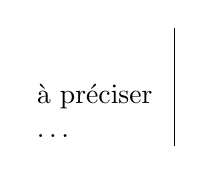
\begin{tikzpicture}
\node[align=left,anchor=east] at (-.15,.45) {à préciser\\$\ldots$};
\draw (0,0)--(0,1.5);
\end{tikzpicture}}}

\margin{\figure{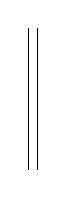
\begin{tikzpicture}\draw (0,0)--(0,1.8);\draw (.12,0)--(.12,1.8);\end{tikzpicture}}}
\uline{Remarque} On voit donc que la position de la filtration p.r. à la stratification ne peut aucunement donner un principe de classification \inserted{des déf.} infinitésimale en car. $p>0$ !
\mspage{17}

\scanpage{19}
La décomposition envisagée (can., fonct.)
\[
\operatorname{DR}^1(A/S)\simeq\underline t_A^\vee+\underline t_{A^*}
\]
vaut pour tt préschéma abélien \uline{ordinaire} sur un $S$ de car. $p>0$, en $=$ temps que les expressions
\[
\underline t_A\simeq\unsure{\Phi|\mathcal L}_A\otimes_{\mathbb F_p}\underline{\mathrm O}_S,
\qquad \underline t_{A^*}\simeq\unsure{\Phi|\mathcal L}_{A^*}\otimes_{\mathbb F_p}\underline{\mathrm O}_S
\]
où $\unsure{\Phi|\mathcal L}_A$, $\unsure{\Phi|\mathcal L}_{A^*}$ sont des faisceaux \inserted{étales} \unsure{loc.} \deleted{const.} libres de rang $g$ ($=\dim\mathrm{rel}$ de $A/S$) de vectoriels sur $\mathbb F_p$. Si $S$ est le spectre d'un corps parfait,
\[
\begin{aligned}
\unsure{\Phi|\mathcal L}_{A^*}&=(\underline t_{A^*})^F
=H^1(\unsure{A|A^*},\underline{\mathrm O}_A)^F
=H^1(A,\mathbb Z/p\mathbb Z)\\
&=\operatorname{Hom}({}_pA,\mathbb Z/p\mathbb Z)
=\deleted{\unsure{\Phi}}\,{}_pA(k)^\vee
\end{aligned}
\]
\[
\left\{\begin{aligned}
\unsure{\Phi|\mathcal L}_{A^*}\deleted{\unsure{F}}(k)&={}_pA(k)^\vee\\
\unsure{\Phi|\mathcal L}_A(k)&={}_pA^*(k)^\vee
\end{aligned}\right.
\]
Donc
\[
\left\{\begin{aligned}
\underline t_A^\vee&=\unsure{\Phi|\mathcal L}_A\deleted{\unsure{(k)}}^\vee\otimes_{\mathbb F_p}k
={}_pA^*(k)\otimes_{\mathbb F_p}k\\
t_{A^*}&={}_pA(k)^\vee\otimes_{\mathbb F_p}k.
\end{aligned}\right.
\]
On a des relations analogues pour $S$ (de car $p>0$) quelconque: l'hyp. sur $A$ implique que
\diagram{\begin{tikzcd}[ampersand replacement=\&]{}_pA\arrow[r] \& S\end{tikzcd}}
s'écrit de façon unique comme composé
\diagram{\begin{tikzcd}[ampersand replacement=\&]{}_pA\arrow[r] \& ({}_pA)_{\text{ét}}\arrow[r] \& S\end{tikzcd}}
de deux morphismes finis loc libres, le premier radiciel surj, le 2ième \uline{étale}.
\mspage{18}

\scanpage{20}
Ceci dit, on a des isom. can.
\[
\left\{\begin{aligned}
\unsure{\Phi|\mathcal L}_A&=({}_pA^*)_{\text{ét}}^\vee\\
\unsure{\Phi|\mathcal L}_{A^*}&=({}_pA)_{\text{ét}}^\vee
\end{aligned}\right.
\]
\uline{NB.} Soit $\varphi$ une polarisation de $A$ (plus gén. une \deleted{\unsure{classe de}} section de $\underline{\operatorname{NS}}_{A/S}$). Alors $\varphi$ définit une \deleted{forme alternée sur}\inserted{section \deleted{\unsure{élément de}} $\varphi'$ de} $\bigwedge^2\operatorname{DR}^1(A/S)$, \deleted{\unsure{ou} alors non dég. Cette forme admet les composantes $\underline H^{10}=\underline t_A^\vee$ et $H^{01}=\underline t_{A^*}$ comme sous-espaces isotropes, et définit donc un accouplement
\diagram{\begin{tikzcd}[ampersand replacement=\&]\underline t_A^\vee\otimes\underline t_{A^*}\arrow[r] \& \underline{\mathrm O}_S\end{tikzcd}}
i.e. un hom
\diagram{\begin{tikzcd}[ampersand replacement=\&]\underline t_{A^*}\arrow[r] \& \underline t_A\end{tikzcd}}.
Cet hom n'est autre que l'hom tangent à
\diagram{\begin{tikzcd}[ampersand replacement=\&]\widetilde\varphi:A\arrow[r,dash] \& A^*\end{tikzcd}}}
\[
\bigwedge^{\unsure{2}}\operatorname{DR}^1(A/S)\simeq
\bigwedge^2\underline t_A^\vee+
\overbrace{\underline t_A^{\unsure{\vee}}\otimes\underline t_{A^*}}^{\operatorname{Hom}(\underline t_A,\underline t_{A^*})}
+\bigwedge^{\unsure{2}}\underline t_{A^*}
\]
Ceci dit, $\varphi'$ est dans le terme médian, et comme tel n'est autre que l'hom tangent
\diagram{\begin{tikzcd}[ampersand replacement=\&]\widetilde\varphi':\underline t_A\arrow[r,dash] \& \underline t_{A^*}\end{tikzcd}}
de
\diagram{\begin{tikzcd}[ampersand replacement=\&]\widetilde\varphi:A\arrow[r] \& A^*\end{tikzcd}}
défini par $\varphi$, qui est déterminé \deleted{\unsure{globalement}}, par \unsure{tensorisation} \deleted{par} $\otimes_{\mathbb F_p}\underline{\mathrm O}_S$, par
\diagram{\begin{tikzcd}[ampersand replacement=\&,column sep=large]
\underline{\unsure{\Phi|\mathcal L}}_A\arrow[r,dash]\arrow[d,equal] \& \underline{\unsure{\Phi|\mathcal L}}_{A^*}\arrow[d,equal]\\
({}_pA^*)_{\text{ét}}^\vee\arrow[r,dash] \& ({}_pA)_{\text{ét}}^\vee
\end{tikzcd}}
transposé de
\diagram{\begin{tikzcd}[ampersand replacement=\&]({}_pA)_{\text{ét}}\arrow[r,dash] \& ({}_pA^*)_{\text{ét}}\end{tikzcd}}
induit par
\diagram{\begin{tikzcd}[ampersand replacement=\&]{}_p\widetilde\varphi:{}_pA\arrow[r,dash] \& {}_pA^*\end{tikzcd}}
$\ldots\ldots$
\mspage{19}

\scanpage{21}
\uline{Re NB.} Soit tjrs $g=\dim\mathrm{rel.}$ de $A/S$, et considérons
\[
\omega_A=\deleted{\unsure{A}}\operatorname{\text{dét}}(\underline t_A)^{-1}
=\bigwedge^g\underline{\unsure{t|\omega}}_A\deleted{\unsure{\vee}}
\]
\inserted{(forme diff. de degré max le long de la section unité)}
C'est un faisceau inv. à $p$-structure non dégénérée, i.e. déduit par ext. des scalaires d'un \deleted{\unsure{faisceau}}\inserted{\deleted{\unsure{fais}} faisceau loc. ct} \deleted{$\unsure{\mathbb F_p\text{-vectoriel}}$} de rang un sur $\mathbb F_p$, savoir $\deleted{\unsure{(}}\operatorname{\text{dét}}({}_pA^*)_{\text{et}}\deleted{\unsure{)}}$. À ce titre, $\omega_A^{\otimes(p-1)}$ admet une section canonique.

Si on ne suppose plus var. $A/S$ ordinaire, et si $U$ est l'ouvert des $s\in S$ tels que $A_s$ soit ordinaire, \deleted{\unsure{tt}} ce qui précède s'applique à $A/U$, en particulier on trouve une section canonique \inserted{$\sigma$} de $L\vert U$, partout $\ne0$.
\deleted{Si $U$ est sch. dense dans $S$, on peut considérer $\sigma$ comme une \deleted{\unsure{par}} pseudo\deleted{\unsure{fonction}}\inserted{pluri-forme} sur $S$ (ou section méromorphe sur $S$), \deleted{\unsure{qui se}}\inserted{mais en}}

Mais en fait, $\sigma$ provient d'une section canonique de $L^{\otimes(p-1)}$ sur $S$ tt entier, définie à l'aide de
\diagram{\begin{tikzcd}[ampersand replacement=\&,column sep=large]t_A^{(p)}\arrow[r,"\pi"] \& t_A\end{tikzcd}}
en passant au dét, d'où
\diagram{\begin{tikzcd}[ampersand replacement=\&,column sep=large](\operatorname{\text{dét}}\underline t_A)^{\otimes p}\arrow[r] \& \operatorname{\text{dét}}\underline t_A\end{tikzcd}}
d'où
\[
\sigma_A\in\Gamma(\operatorname{\text{dét}}\underline t_A)^{1-p}=\Gamma\omega_A^{(p-1)}.
\]
\mspage{20}

\scanpage{22}
Cette section mérite le nom de \uline{invariant de Hasse} de $A$. L'ens des zéros de cette section est exactement l'ens des $s$ tels que $A_s$ soit \uline{non ordinaire}.

Quelles sont les relations entre $\omega_A$ et $\omega_{A^*}$ ? On a, grâce à la suite exacte
\diagram{\begin{tikzcd}[ampersand replacement=\&,column sep=small]
\unsure{0}\arrow[r,dash] \& \underline t_A^\vee\arrow[r] \& \operatorname{DR}^1(A/S)\arrow[r,dash] \& \underline t_{A^*}\arrow[r,dash] \& 0
\end{tikzcd}}
la relation
\diagram{\begin{tikzcd}[ampersand replacement=\&,column sep=large,row sep=large]
\operatorname{\text{dét}}\underline t_A^\vee\otimes\operatorname{\text{dét}}\underline t_{A^*}\arrow[r,phantom,"\simeq" description] \& \operatorname{\text{dét}}\operatorname{DR}^1(A/S)\arrow[d,phantom,"\rotatebox{90}{$\simeq$}" description] \&\\
\& \operatorname{DR}^{2g}(A/S)\arrow[r,phantom,"\simeq" description] \& \underline{\mathrm O}_S
\end{tikzcd}}
donc on aura
\[
\omega_A\cdot\omega_{A^*}^\vee\simeq\underline{\mathrm O}_S
\]
i.e. on a un isom can.
\[
\omega_A\simeq\omega_{A^*}
\]
Je dis que \uline{cet isom est compatible avec les $p^{-1}$-structures}, \uline{donc transforme $\sigma_A$ en $\sigma_{A^*}$, et dans le cas $A$ ordinaire}, induit un isom
\[
\operatorname{\text{dét}}({}_pA)_{\text{ét}}\simeq\operatorname{\text{dét}}({}_pA^*)_{\text{ét}}.
\]
\mspage{21}

\scanpage{23}
Il s'impose de regarder \unsure{églt}, si $A$ est ordinaire
\[
T_p(A)_{\text{et}}=\varprojlim\deleted{\unsure{T_p}}({}_{p^{\unsure{\nu|n}}}A)_{\text{et}}
\]
(NB. $T_p(A)$ est une extension
\diagram{\begin{tikzcd}[ampersand replacement=\&,column sep=small]
0\arrow[r] \& T_p(A)_{\mathrm{rad}}\arrow[r] \& T_p(A)\arrow[r,dash] \& T_p(A)_{\text{et}}\arrow[r,dash] \& 0
\end{tikzcd}}
On sait, par dualité de Cartier, que dans la suite exacte correspondante
\diagram{\begin{tikzcd}[ampersand replacement=\&,column sep=small]
\unsure{0}\arrow[r,dash] \& T_p(A^*)_{\mathrm{rad}}\arrow[r,dash] \& T_p(A^*)\arrow[r,dash] \& T_p(A^*)_{\text{et}}\arrow[r,dash] \& 0
\end{tikzcd}}
les termes médians sont duaux l'un de l'autre, et \deleted{plus précisément} cette dualité est compatible avec filtrations, donc
\[
\begin{aligned}
T_p(A)_{\mathrm{rad}}&\simeq D(T_p(A^*)_{\text{et}})\\
T_p(A^*)_{\mathrm{rad}}&\simeq D(T_p(A)_{\text{et}})
\end{aligned}
\]
donc la connaissance de $T_p(A)_{\text{et}}$ et $T_p(A^*)_{\text{et}}$ permet de reconstituer les \uline{deux} facteurs de $T_p(A)$, donc $T_p(A)$ si la base est parfaite [en général, il y aurait lieu d'expliciter la structure d'extension $\ldots$].

On aurait envie d'établir un isom can. \deleted{fonctoriel}
\mspage{22}

\scanpage{24}
\diagram{\begin{tikzcd}[ampersand replacement=\&,column sep=large]
\operatorname{\text{dét}}T_p(A)_{\text{ét}}\arrow[r,"\sim"] \& \operatorname{\text{dét}}T_p(A^*)
\end{tikzcd}}
[\deleted{Soit} Si on a $\ell\ne p$ au lieu de $p$, on a bien
\diagram{\begin{tikzcd}[ampersand replacement=\&,column sep=large]
\operatorname{\text{dét}}T_\ell(A)\arrow[r,phantom,"\simeq" description,"\alpha_\ell"] \& \operatorname{\text{dét}}T_\ell(A^*)\arrow[r,phantom,"\simeq" description] \& \mathbb Z_\ell(g)
\end{tikzcd}}]
\deleted{car $T_\ell(A^*)\simeq\deleted{\operatorname{\text{dét}}}T_\ell(\unsure{A^*|A})^\vee\otimes\mathbb Z_\ell(1)$ donc $\operatorname{\text{dét}}T_\ell(A^*)\simeq\operatorname{\text{dét}}T_\ell(A)$ (Choisissons une polarisation)}

Si $\varphi$ est une polarisation de $A$, définissant
\diagram{\begin{tikzcd}[ampersand replacement=\&]\widetilde\varphi:A\arrow[r,dash] \& A^*\end{tikzcd}}
d'où
\diagram{\begin{tikzcd}[ampersand replacement=\&]T_\ell(\widetilde\varphi):T_\ell(A)\arrow[r,dash] \& T_\ell(A^*)\end{tikzcd}},
\diagram{\begin{tikzcd}[ampersand replacement=\&,column sep=large]
\operatorname{\text{dét}}T_\ell(\widetilde\varphi):\operatorname{\text{dét}}T_\ell(A)\arrow[r,"\beta_\ell(\varphi)"] \& \operatorname{\text{dét}}T_\ell(A^*)
\end{tikzcd}},
alors l'isom $\alpha_\ell$ n'est autre que $\beta_\ell(\varphi)/\deg\varphi$. En s'inspirant de cette formule, on définira;
\diagram{\begin{tikzcd}[ampersand replacement=\&,column sep=large]
\beta_p(\varphi)=\operatorname{\text{dét}}(T_p(\widetilde\varphi)_{\text{ét}}):\operatorname{\text{dét}}T_p(A)_{\text{ét}}\arrow[r] \& \operatorname{\text{dét}}T_p(A^*)_{\text{ét}}
\end{tikzcd}}
et on considère
\[
\alpha_p(\varphi)=\beta_p(\varphi)/\sqrt{\deg\widetilde\varphi}:
\]
\diagram{\begin{tikzcd}[ampersand replacement=\&,column sep=large]
\operatorname{\text{dét}}T_p(A)_{\text{ét}}\otimes\mathbb Q_{\unsure{\ell|p}} \& \operatorname{\text{dét}}T_p(A^*)_{\text{ét}}\inserted{\otimes\mathbb Q_{\unsure{\ell|p}}}\arrow[l]
\end{tikzcd}}
À prouver: a) $\alpha_p(\varphi)$ ne dépend pas de $\varphi$.

\deleted{est \unsure{pratiquement} formelle de ceci}
\deleted{\uline{Lemme} Soit $u$ un \deleted{\unsure{autom}}\deleted{\unsure{endom}}\inserted{endom} de $A$, d'où
\diagram{\begin{tikzcd}[ampersand replacement=\&,column sep=large]
[\operatorname{\text{dét}}T_p(u)_{\text{ét}}:\operatorname{\text{dét}}T_p(A)_{\text{ét}}\deleted{\unsure{\mathbf Z_p}}\arrow[r] \& \operatorname{\text{dét}}T_p(A)_{\text{ét}}]\in\mathbb Z_p.
\end{tikzcd}}
On a
\[
\left\{\begin{aligned}
&\deg u\text{ est un carré parfait}\\
&\operatorname{\text{dét}}(T_p(u)_{\text{ét}})=\sqrt{\deg u}
\end{aligned}\right.
\]
i.e.
\[
\deg u=(\operatorname{\text{dét}}(T_p(u)_{\text{ét}}))^2
\]
\uline{et} $\operatorname{\text{dét}}T_p(u)_{\text{ét}}$ est un entier $>0$}
\margin{\uline{faux}}
\mspage{23}

\scanpage{25}
En effet, soit $\psi$ une autre polarisation, donc $\widetilde\psi=\widetilde\varphi\circ u$, où $u\in\operatorname{End}(A)\otimes_{\mathbb Z}\mathbb Q$, \deleted{le} et la condition $\widetilde\psi'=-\widetilde\psi$ (jointe à $\widetilde\varphi'=-\widetilde\varphi$) donne
\[
\begin{array}{ccc}
u'\widetilde\varphi'=-\widetilde\varphi u & \text{i.e.} & u'=\widetilde\varphi u\widetilde\varphi^{-1}.\\
\Vert &&\\
-u'\widetilde\varphi &&
\end{array}
\]
On veut prouver [posant $\delta(\widetilde\varphi)=\sqrt{\deg\widetilde\varphi}$, $\alpha_p(\widetilde\varphi)=\Delta(\widetilde\varphi)$]
\[
\begin{array}{ccc}
\Delta(\widetilde\psi)/\delta(\unsure{\widetilde\varphi|\widetilde\psi})&=&\Delta(\widetilde\varphi)/\delta(\widetilde\varphi)\\
\Vert&&\\
\Delta(\widetilde\varphi)\cdot\Delta(u)/\delta(\widetilde\varphi)\delta(u)&&
\end{array}
\]
qui équivaut à: $\Delta(u)/\delta(u)=1\deleted{\unsure{2}}$. Or par \unsure{lemme} on a
\[
\begin{array}{c}
\deleted{\Delta}\;\Delta(u)\Delta(u^*)=\delta(u)^2\\
\hfill\Vert\\
\hfill\deg u
\end{array}
\]
d'autre part, comme $u^*=\widetilde\varphi u\widetilde\varphi^{\deleted{\unsure{*}}\inserted{-1}}$, on a ici $\Delta(u^*)=\Delta(u)$, donc \deleted{$\unsure{\Delta(u)}$}
\[
\Delta(u)^2=\delta(u)^2
\]
d'où $\Delta(u)=\pm\delta(u)$. Il faut encore avoir le signe, il faut \deleted{\unsure{pour dire}} donc sur $\operatorname{End}(A)\otimes_{\mathbb Z}\mathbb Q$, muni de l'involution $u\unsure{\longmapsto|\sim}u'=\widetilde\varphi u\widetilde\varphi^{-1}$, prouver que $u>0$ (i.e. \deleted{\unsure{réellement}} $u=\sum v_iv_i'$) \deleted{$u=u'$} implique $\Delta(u)={\text{\uuline{\uline{$+$}}}}\delta(u)$ [NB. $\delta(u)$ est bien défini, car $\deg u$ est bien un carré parfait si $u=u'$]
\deleted{Or l'identité $\Delta(u)^2=\delta(u)$ est une identité dans}
\mspage{24}

\scanpage{26}
\deleted{
\deleted{Comme $T_p(u)$ et $T_p(u^*)$ sont}

En effet, d'après la théorie $p$-adique \inserted{de Serre} (ou th. cohomologique de Weil, on aura
\[
(*)\quad \deg u=\det T_p(u)_{\text{ét}}\det T_p(u^*)_{\text{ét}},
\]
\margin{$\unsure{-\,=}$}
et il reste à prouver que
\[
1^\circ)\quad T_p(u)_{\text{ét}}=T_p(u^*)_{\text{ét}}
\]
\margin{\figure{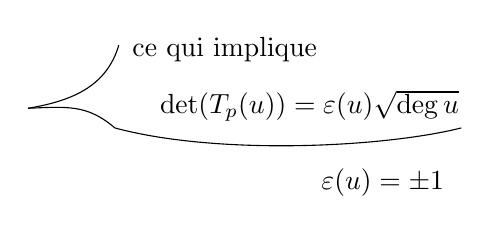
\begin{tikzpicture}[x=1cm,y=1cm]
\draw (0,0) .. controls (.6,.1) and (1,.3) .. (1.15,.8);
\draw (0,0) .. controls (.5,.02) and (.75,.05) .. (1.1,-.25) .. controls (2.4,-.6) and (4.5,-.5) .. (5.5,-.25);
\node[anchor=west] at (1.2,.75) {ce qui implique};
\node[anchor=west] at (1.55,.03) {$\det(T_p(u))=\varepsilon(u)\sqrt{\deg u}$};
\node[anchor=west] at (3.6,-.95) {$\varepsilon(u)=\pm1$};
\end{tikzpicture}}}
\[
2^\circ)\quad\varepsilon(u)=1
\]
D'ailleurs on peut \inserted{se borner à} supposer $u\in\operatorname{Hom}(A,A)\otimes_{\mathbb Z}\mathbb Q\underset{\unsure{\varepsilon}}{=}E$, et alors $\varepsilon$ est un hom
\[
E^*\longrightarrow(+1,-1),\quad\deleted{\unsure{de gr.}}
\]
qui est une fonction rationnelle (quotient de deux fonctions
\deleted{\unsure{on sait} \unsure{que tout tel hom.} \unsure{est égal}}
}

\mspage{25}

\scanpage{27}
Or pour $u$ variable, $\Delta(u)$ est un polynôme dans $\unsure{\mathbb Z|\mathbb Q}_p[T]$ ($T=(T_1\cdots T_{\unsure{N|\alpha}})$, $N=\deleted{\dim}\operatorname{rg}_{\mathbb Z}\operatorname{End}(A)_{\unsure{\mathrm{herm}|\mathrm{hom}}}$), qui, on vient de le voir, prend des valeurs entières pour des valeurs entières des variables. Donc $\Delta(u)$ est un polynôme à coeff. \deleted{entiers} dans $\mathbb Q$ (et non seulement dans $\mathbb Q_p$), \deleted{\unsure{donc même à coeff.} dans $\mathbb Z_{(p\mathbb Z)}$ (car $\mathbb Z_p[T]\cap\mathbb Q[T]=\mathbb Z[T]$, $\mathbb Z_p\cap\mathbb Q=\mathbb Z_{(p\mathbb Z)}$).}
Il faut prouver que ses valeurs sur le cône des $u>0$ \deleted{sont} $\geq0$, et \deleted{\unsure{pour que}} il suffit de le prouver quand on passe de $\mathbb Q$ à $\mathbb R$. Mais alors tt élém $\geq0$ est un carré d'un élém hermitien \inserted{$\unsure{v|w}$} $\geq0$, donc
\[
\Delta(u)=\Delta(\unsure{v|w}^2)=\unsure{\Delta|\delta}(\unsure{v|w})^2\in\mathbb R^2=\mathbb R^+,
\]
cqfd.

b) $\alpha_p(\varphi)$ induit bien un \uline{isom} de $\det T_p(A)_{\text{ét}}$ avec $\det T_p(A^*)_{\text{ét}}$. Cela \deleted{\unsure{exprime que ces deux}}
\inserted{équivaut à la relation}
\deleted{(i) $\alpha_p(\varphi)$ applique $\det T_p(A)_{\text{ét}}$ sur $\det T_p(A^*)_{\text{ét}}$, $\beta_p(\varphi)$}
\[
v_p\bigl(\operatorname{card}(\operatorname{Coker}\deleted{\unsure{\varphi}}T_p(\widetilde\varphi)_{\text{ét}})\bigr)=v_p\bigl(\sqrt{\deg\widetilde\varphi}\bigr)
\]
Or on a évidemment.

\mspage{26}

\scanpage{28}
\[
\operatorname{Coker}T_p(\widetilde\varphi)_{\text{ét}}\simeq(\operatorname{Ker}\unsure{(}\widetilde\varphi)(p)_{\text{ét}}
\]
Or on sait que $\operatorname{Ker}\widetilde\varphi$ est autodual, donc $(\operatorname{Ker}\widetilde\varphi)(p)_{\text{ét}}$ est dual de $(\operatorname{Ker}\widetilde\varphi(p))_{\mathrm{rad}}$, donc $=$ cardinal, d'où la relation
\[
\begin{array}{rcl}
\bigl(\operatorname{card}(\operatorname{Ker}\widetilde\varphi)(p)_{\text{ét}}\bigr)^2&=&\operatorname{card}\operatorname{Ker}(\widetilde\varphi(p))\\
&&\rotatebox{90}{$=$}\\
&& (\deg\widetilde\varphi)(p).
\end{array}
\]
d'où la relation envisagée \ldots\ldots\ . Cela définit bien un isom canonique
\diagram{$(*)$\quad\fbox{\begin{tikzcd}[ampersand replacement=\&,column sep=huge]
\det T_p(A)_{\text{ét}}\arrow[r,"\sim","\alpha_A"']\&\det T_p(A^*)_{\text{ét}}
\end{tikzcd}}}
compatible aux changt de base, et isom. en $A$.

[ Si $u$ est un autom. de $A$, et $\check u=u^{*-1}$ son contragredient, on aura
\[
\alpha\,\det T_p(u)_{\text{ét}}=\det T_p(\check u)_{\text{ét}}\alpha,
\]
donc en identifiant les dét s à des élém de $\mathbb Z_p$ \deleted{\unsure{(i)}}, on aura
\[
\begin{array}{rcl}
\det T_p(u)_{\text{ét}}&=&\det T_p(u^{*-1})_{\text{ét}}\\
&&\rotatebox{90}{$=$}\\
&& (\det T_p(u^*))^{-1}
\end{array}
\]
donc
\[
\boxed{\det T_p(u)_{\text{ét}}\,\inserted{\det}T_p(u^*)_{\text{ét}}=1}\qquad\text{\uline{$u$ un autom de $A$}}
\]
]

\margin{\figure{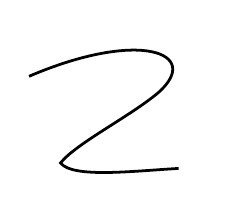
\begin{tikzpicture}[x=1cm,y=1cm]
\draw[line width=1pt] (0,1.4) .. controls (1.4,2) and (2.2,1.7) .. (1.65,1.2) .. controls (1.3,.9) and (.6,.55) .. (.4,.3) .. controls (.55,.1) and (1.35,.2) .. (1.9,.23);
\end{tikzpicture}}}
Attention, si $u$ est un endom de $A$, on aura en général
\[
\det T_p(u)\ne\det T_p(u^*)
\]
\mspage{27}

\scanpage{29}
$=$ si $A$ courbe elliptique sur corps alg. clos; donc l'isom can n'est \uline{pas} fonctoriel pour les hom de schémas abéliens de $=$ dimension [dans la mesure où ça pourrait avoir un sens, les deux foncteurs n'étant pas de $=$ variance en $A$\ldots]. Cependant, \deleted{\unsure{si $u$ est} \illegible{2} \unsure{A.B.} \illegible{2}}
\[
\boxed{\det T_p(u)_{\text{ét}}\,\det T_p(u^*)_{\text{ét}}=\deg u}
\]
\margin{Vaut aussi (via \unsure{identifications} \unsure{permises|possibles}) pour des Sch.A. de $=$ dimension}

c) Il faudrait vérifier que
\[
\alpha_{A^*}=\alpha_A^{-1}
\]
[ aux signes (?)\ldots]. Noter aussi la compatibilité par sommes de V.A.\ \ldots

 d) L'isom $({}_pA)_{\text{ét}}\longrightarrow({}_pA^*)_{\text{ét}}$ induit par $\alpha_A$ est bien celui déduit plus haut de la dualité en cohomologie de DeRham (à vérifier \ldots).

\mspage{28}

\cotefile{4}
\scanpage{1}
\figure{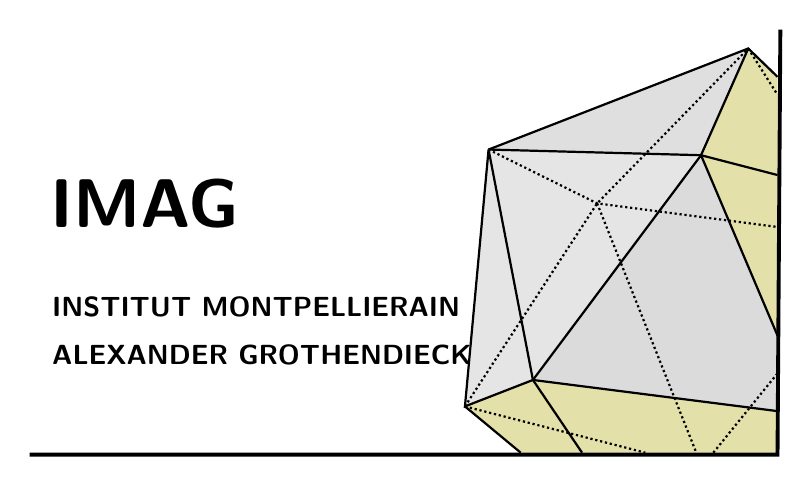
\begin{tikzpicture}[x=.012cm,y=-.012cm,line width=.8pt]
\node[anchor=west,font=\sffamily\bfseries\Huge] at (20,195) {IMAG};
\node[anchor=west,font=\sffamily\bfseries] at (22,305) {INSTITUT MONTPELLIERAIN};
\node[anchor=west,font=\sffamily\bfseries] at (22,355) {ALEXANDER GROTHENDIECK};
\fill[gray!25] (495,138)--(770,31)--(720,144)--cycle;
\fill[gray!20] (495,138)--(720,144)--(542,382)--(470,410)--cycle;
\fill[gray!28] (720,144)--(801,335)--(801,415)--(542,382)--cycle;
\fill[olive!25] (770,31)--(801,61)--(801,335)--(720,144)--cycle;
\fill[olive!25] (470,410)--(542,382)--(801,415)--(801,459)--(529,459)--cycle;
\draw (495,138)--(770,31)--(801,61);
\draw (495,138)--(720,144)--(770,31);
\draw (720,144)--(801,165);
\draw (495,138)--(470,410)--(542,382)--(495,138);
\draw (542,382)--(720,144)--(801,335);
\draw (470,410)--(529,459);
\draw (542,382)--(594,459);
\draw (542,382)--(801,415);
\draw[densely dotted] (495,138)--(610,195)--(801,220);
\draw[densely dotted] (470,410)--(610,195)--(770,31);
\draw[densely dotted] (610,195)--(715,459);
\draw[densely dotted] (470,410)--(661,459);
\draw[densely dotted] (733,459)--(801,375);
\draw[densely dotted] (770,31)--(801,80);
\draw[line width=1.4pt] (9,461)--(801,461)--(804,11);
\end{tikzpicture}}

\scanpage{2}
\begin{center}
INSTITUT\\
DES HAUTES ÉTUDES SCIENTIFIQUES\\
\rule{1.2cm}{.4pt}
\end{center}
8.4.4.

\uline{NB}

 a) $F$ opérant sur $H^i(X)\otimes_W k$ pour $i>n$ est \uline{nilpotent}, donc aussi opérant sur $\operatorname{Tors}^i(X)\otimes_W k$ ou sur $\operatorname{Tor}_{\unsure{1}}^W(H^i(X),k)\simeq{}_p\operatorname{Tors}^i(X)$.

On a $H^n(X,\underline{O}_X)_{\mathrm{ss}}\unsure{\xleftarrow{\sim}|\simeq}(H^n(X)\otimes_W k)_{\mathrm{ss}}$ d'où
\diagram{\begin{tikzcd}[ampersand replacement=\&,column sep=small]
0\arrow[r]\& (\unsure{\operatorname{Tors}|H}^{n}_{\unsure{\mathrm{ss}}}(X)\otimes k)_{\mathrm{ss}}\arrow[r]\&H^n(X,\underline{O}_X)_{\mathrm{ss}}\arrow[r]\& (H^n_{\mathrm{lib}}(X)\otimes_{\unsure{\mathrm{ss}}}k)_{\mathrm{ss}}\arrow[r]\&0
\end{tikzcd}}
\margin{$(*)$ \unsure{$T_{\mathrm{lib}}^n(X)$}}

 b) $V$ opérant sur $H^i(X)\otimes_W k$ pour $i<n$ est nilpotent, et aussi opérant sur $\operatorname{Tors}^i(X)\otimes_W k$ et ${}_p\operatorname{Tors}^i(X)$ pour \uuline{$i\leq n$}. On a
\margin{$(**)$}
\diagram{\begin{tikzcd}[ampersand replacement=\&,column sep=small]
0\arrow[r]\& (H^n_{\mathrm{lib}}(X)\otimes k)_{\unsure{\mathrm{ss}}}^{\mathrm{ss}}\arrow[r]\&H^0(X,\underline{\Omega}_X^n)^{\mathrm{ss}}\arrow[r,Rightarrow]\&{}_p\operatorname{Tors}^{n+1}(X)_{\unsure{\mathrm{ss}}}^{\mathrm{ss}}\arrow[r]\&0\unsure{\operatorname{Tor}}
\end{tikzcd}}

Sans doute $(*)$ et $(**)$ sont transposés l'un de l'autre \ldots

\uline{Notation}\quad L'indice ${}_{\mathrm{ss}}$ indique partie semi-simple pour $F$\\
L'exposant ${}^{\mathrm{ss}}$ \rule{7cm}{.3pt} $V$

\mspage{1}

\scanpage{3}
8. \uline{Une estimation (heuristique) du nombre des valeurs propres de frobe-}\\
\uline{nius dans la cohomologie évanescente qui sont des unités $p$-adiques.}

8.1. Soit $X$ un schéma lisse et propre sur le corps parfait $k$, \inserted{de car. $p>0$} et soit $W$ l'anneau des vecteurs de Witt sur $k$. Si on dispose d'une bonne théorie \unsure{de} la cohomologie cristalline $H(X)$ (au sens des catégories dérivées), on \unsure{devra} avoir la relation suivante avec la cohomologie de De Rham
\[
(8.1.1)\qquad H_{\mathrm{DR}}(X)=H(X)\overset{\inserted{L}}{\otimes}_W k
\]
(isomorphisme dans la catégorie dérivée des $k$-modules). On en déduit \unsure{une} formule des coefficients universels: suitesexactes
\diagram{$(8.1.2)$\quad\begin{tikzcd}[ampersand replacement=\&,column sep=small]
0\arrow[r]\&H^i(X)\otimes_W k\arrow[r,dash]\&H^i_{\mathrm{DR}}(X)\arrow[r]\&\operatorname{Tor}_1^W(H^{i+1}(X),k)\arrow[r]\&0
\end{tikzcd}.}
Ce sont des suites exactes fonctorielles en $X$, tout comme l'isomorphisme (8.1.1). Sauf erreur, \deleted{\unsure{tout}} ceci marche dès maintenant pour $p\ne2$, grâce à Berthelot.

\margin{[ On conclut, grâce à \unsure{8.4.3},
\diagram{\begin{tikzcd}[ampersand replacement=\&,column sep=small]
0\arrow[r]\&(H^i(X)\otimes_W k)_{\mathrm{ss}}\arrow[r]\&H^i(X,\underline{O}_X)_{\mathrm{ss}}\arrow[r]\arrow[d,phantom,"\text{(nul si }i>n\text{)}"]\&({}_p\operatorname{Tors}^{i+1}(X))_{\mathrm{ss}}\arrow[r]\arrow[d,phantom,"\text{nul si }i\geq n"]\&0\\
\&\&\phantom{H}\&\phantom{H}\&
\end{tikzcd}}
]}
\margin{et
\diagram{\begin{tikzcd}[ampersand replacement=\&,column sep=small]
0\arrow[r]\&(H^{\unsure{i+n}}(X)\otimes_W k)^{\mathrm{ss}}\arrow[r]\&H^i(X,\Omega_X^n)^{\mathrm{ss}}\arrow[r]\&({}_p\operatorname{Tors}^{i+n+1}(X))^{\mathrm{ss}}\arrow[r]\&0
\end{tikzcd}}
où l'indice ${}_{\mathrm{ss}}$ signifie la partie semi-simple pour $F_X=F_X^*\sigma$\\
et \unsure{où} l'exposant ${}^{\mathrm{ss}}$ \rule{6cm}{.3pt} $V_X=\sigma^{-1}F_{X*}$ ]}

Si maintenant $Y$ est une section hyperplane de \deleted{degré assez élevé de} $X$ (supposée maintenant $\subset P_k^r$), on trouve une suite exacte analogue pour $Y$, et un homomorphisme \inserted{$u=(u_0,u_1,u_2)$} de la première dans la seconde. Le diagramme du serpent nous donne alors une suite exacte
\diagram{$(8.1.3)$\quad\begin{tikzcd}[ampersand replacement=\&,column sep=small,row sep=large]
\inserted{0}\arrow[r]\&\inserted{\operatorname{Ker}u_0}\arrow[r]\&\inserted{\operatorname{Ker}u_1}\arrow[dll,bend left=15]\&\&\\
\inserted{\operatorname{Ker}u_2}\arrow[r]\&E(Y)\otimes_W k\arrow[r]\&E_{\mathrm{DR}}(Y)\arrow[r]\arrow[d,phantom,"\rotatebox{90}{$=$}"]\&\operatorname{Coker}u_2\arrow[r]\&0\\
\&\&\inserted{\operatorname{Coker}u_1}\&\&
\end{tikzcd},}
où on a posé
\[
E(Y)=\operatorname{Coker}(H^{n-1}(X)\xrightarrow{\inserted{u_0}}H^{n-1}(Y)),\qquad E_{\mathrm{DR}}(Y)=\operatorname{Coker}(H^{n-1}_{\mathrm{DR}}(X)\xrightarrow{\inserted{u_1}}H^{n-1}_{\mathrm{DR}}(Y)),
\]
$X$ étant supposée connexe de dimension $n$, enfin $u_2$ désigne l'application
\[
(8.1.4)\qquad u_{\inserted{2}}:\operatorname{Tor}_1^W(H^n(X),k)\longrightarrow\operatorname{Tor}_1^W(H^n(Y),k).
\]

\deleted{\margin{\figure{\begin{tikzpicture}[x=1cm,y=1cm]
\node[draw,ellipse,minimum width=.85cm,minimum height=2cm] (n) at (0,0) {8.2.};
\draw (-.15,-.6)--(-.75,-1.7);
\end{tikzpicture}}}
Noter que $\operatorname{Tor}_1^W(-,k)$ est isomorphe à $\operatorname{Hom}_W(k,-)$ (éléments de $-$ annulés par $pW$), et que \deleted{\unsure{$H^n($}} $\operatorname{Tors}^n(Y)$ ($=$\deleted{\unsure{(}}sous-module de torsion de $Y$) est dual (si on admet la \uline{dualité de Poincaré} habituelle pour la cohomologie cristalline, y compris les formules pour la torsion) de $\operatorname{Tors}^{n-1}(Y)$, et}
\margin{il est maladroit d'utiliser ici la dualité de Poincaré \deleted{\illegible{1}}}

\mspage{2}

\scanpage{4}
\deleted{par suite le deuxième membre de (8.1.4) est canoniquement dual à $\operatorname{Tors}^{n-1}(Y)\otimes_W k$. De même le premier membre est canoniquement \deleted{isomorphe à}\inserted{dual de} $\operatorname{Tors}^{n+1}(X)\otimes_W k$, et enfin l'homomorphisme $u$ est transposé de l'\unsure{homomorphisme}
\[
(8.2.\unsure{1})\qquad u'_2:\operatorname{Tors}^{n-1}(Y)\otimes_W k\longrightarrow\operatorname{Tors}^{n+1}(X)\otimes_W k
\]
induit par l'homomorphisme de Gysin
\[
H^{n-1}(Y)\longrightarrow H^{n+1}(X).
\]
Par suite, les termes $\operatorname{Ker}u_2$ et $\operatorname{Coker}u_2$ dans (8.1.3) peuvent \unsure{d'interpréter|s'interpréter} \deleted{comme} respectivement comme \deleted{\unsure{Coker}} les duals de $\operatorname{Coker}u'_2$ et $\operatorname{Ker}u'_2$.}

8.3. Considérons l'homomorphisme induit par l'inclusion \inserted{$Y\to X$,}
\[
u_{\unsure{0}}:H^{n-1}(X)\longrightarrow H^{n-1}(Y).
\]
\deleted{Sauf erreur,} Dans la situation analogue \deleted{sur le corps des complexes,}\inserted{en cohomologie $\ell$-adique ($\ell\ne p$)} \uline{\deleted{les assertions}\inserted{théorème} de Lefschetz} \deleted{dans son livre ``L'Analysis Situs\ldots''}\inserted{faible (pour les coefficients $\mathbb Z/\ell^{\deleted{\unsure{n}}}\mathbb Z$)} impliquent que \uline{le conoyau} $E(Y)$ \uline{est sans torsion}, ce qui implique en \unsure{particulier} que $u_0$ induit un \uline{isomorphisme}
\[
(8.3.1)\qquad\operatorname{Tors}^{n-1}(X)\xrightarrow{\sim}\operatorname{Tors}^{n-1}(Y).
\]
\margin{\figure{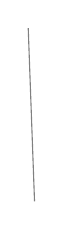
\begin{tikzpicture}\draw[gray] (0,0)--(-.08,2.2);\end{tikzpicture}}}

Nous admettrons que ces relations restent valables dans le cas de la cohomologie cristalline. Alors l'homomorphisme (8.2.1) s'interprète comme l'homomorphisme
\[
(8.3.2)\qquad u''_2:\operatorname{Tors}^{n-1}(X)\otimes_W k\longrightarrow\operatorname{Tors}^{n+1}(X)\otimes_W k
\]
induit par l'homomorphisme $H^{n-1}(X)\to H^{n+1}(X)$, cup-produit par la classe de polarisation de $X\subset P_k^r$. La chose importante pour nous est que ce morphisme (donc son Ker) ne dépend plus du choix de $Y$, donc \deleted{aussi du}\deleted{\unsure{il en est de même}}\inserted{le} dernier terme de (8.1.3) \deleted{ne dépend} (qui est le dual de ce Ker) ne dépend plus de $Y$. Un autre point important est que, $E(Y)$ étant sans torsion, il a même rang que $E(Y)\otimes_W k$ intervenant dans (8.1.3) (et en particulier, si on a un endomorphisme de $E(Y)$, par exemple un frobenius, les valeurs propres de l'endomorphisme induit de $E(Y)\otimes k$ sont bien les réductions

\mspage{3}

\scanpage{5}
mod $p$ des valeurspropres de l'endomorphisme donné de $E(Y)$). Enfin, (et c'est un petit luxe supplémentaire moins important pour nous, car seul les trois derniers termes de (8.1.3) sont pour nous vraiment importants du point de vue assymptotique \ldots) \deleted{\unsure{on aura $\operatorname{Ker}u$}} le \unsure{premier} terme $\operatorname{Ker}u_0$ dans (8.1.3) est nul:
\[
(8.3.3)\qquad\operatorname{Ker}u_0=0.
\]

8.4. Notons maintenant que l'on a des applications semi-linéaires Frob opérant fonctoriellement sur tous les espaces de cohomologie \unsure{envisagés}, et en particulier sur \deleted{\unsure{ceux}}\inserted{les termes} intervenant dans (8.1.3), qui sont donc des vectoriels de dimension finie sur $k$ avec endomorphisme $p$-linéaire. Considérons, pour un tel vectoriel $V$, le plus grand sous-espace \unsure{vectoriel} stable $V_{\mathrm{SS}}$ (partie ``semi-simple'' de $V$) stable par $F_V$, et sur lequel $F_V$ soit \inserted{``semi-simple'' i.e.} surjectif (NB $k$ est parfait); \deleted{\unsure{Le foncteur}} il revient au,même de dire que $F$ est surjectif sur ce sous-espace, et \uline{nilpotent}\deleted{\unsure{r}} sur le quotient. Pour $V$ variable, la formation de $V_{\mathrm{SS}}$ est un foncteur exact en $V$. Ainsi, la suite exacte (8.1.3) nous donne, compte tenu de (8.3.3), la suite exacte d'espace vectoriels à opérateurs $p$-linéaires semi-simples:
\diagram{$(8.4.1)$\quad\begin{tikzcd}[ampersand replacement=\&,column sep=small,row sep=large]
\&\&\inserted{({}_p\operatorname{Tors}^n(X))_{\mathrm{ss}}}\&\&\&|[draw,ellipse]|\inserted{0\ \text{en vertu de 8.4.4.}}\arrow[lll,bend right=15]\arrow[d,phantom,"\rotatebox{90}{$=$}"]\&\\
0\arrow[r]\&(\operatorname{Ker}u_1)_{\mathrm{SS}}\arrow[r]\&(\operatorname{Ker}u_2)_{\mathrm{SS}}\arrow[u,phantom,"="]\arrow[r]\&(E(Y)\otimes_W k)_{\mathrm{SS}}\arrow[r]\&E_{\mathrm{DR}}(Y)_{\mathrm{SS}}\arrow[r]\&(\operatorname{Coker}u_2)_{\mathrm{SS}}\arrow[r]\&0
\end{tikzcd}.}

\inserted{8.4.2.} D'après la théorie de structure des vectoriels à opération $p$-linéaire semi-simple, \deleted{qui}\inserted{ceux-ci} peuvent s'interpréter aussi comme des Modules libres \unsure{de} type fini sur le faisceau d'anneaux étale constant $\underline F_p$ (corps premier à $p$ éléments), ou encore \deleted{\unsure{comme}} (une fois choisie une clôture séparable) comme des \deleted{\unsure{$G$-$\underline F_p$}} représentations de $G=\operatorname{Gal}(\bar k/k)$ sur des vectoriels de \unsure{dimension} finie sur $\underline F_p$. Dans cette catégorie il y a une autodualité, qui \unsure{s'interprète} indifféremment en termes de dualité d'espaces de dimension finie sur $k$ avec opération $p$-linéaire semi-simple, ou en termes de dualité de

\mspage{4}

\scanpage{6}
\deleted{\unsure{$G$-$\underline F_p(G)$-Modules}} Modules de représentations de $G$ sur $\underline F_p$. Alors les termes $(\operatorname{Coker}u_2)_{\mathrm{SS}}$ et $(\operatorname{Ker}u_2)_{\mathrm{SS}}$ peuvent s'interpréter aussi comme les duals de $(\operatorname{Ker}u''_2)_{\mathrm{SS}}$ et de $(\operatorname{Coker}u''_2)_{\mathrm{SS}}$, $u''_2$ défini dans (8.3.2). Enfin \deleted{\unsure{$(\operatorname{Ker}u_1)_{\mathrm{SS}}$}} $(\operatorname{Coker}u_1)_{\mathrm{SS}}$ et $(\operatorname{Ker}u_1)_{\mathrm{SS}}$ ont aussi une interprétation simple, grâce au

\margin{\figure{\begin{tikzpicture}\draw[gray] (0,0)--(0,2.6);\end{tikzpicture}}}
\uline{Lemme} 8.4.\unsure{3}. Soit $X$ un schéma propre sur un corps $k$, de car. $p>0$. Alors pour tout $i\in\underline Z$, l'homomorphisme d'augmentation \deleted{\unsure{H}}
\[
H^i_{\mathrm{DR}}(X)\longrightarrow H^i(X,\underline O_X)
\]
induit un isomorphisme sur les parties semi-simples (pour l'opération $p$-linéaire de Frobenius).

Ceci résulte aussitôt de la suite spectrale de Hodge
\[
E_1^{a,b}=H^b(X,\underline\Omega^a_{X/k})\Longrightarrow H^\bullet_{\mathrm{DR}}(X),
\]
compte tenu que Frob opère \deleted{semi} $p$-linéairement sur cette suite spectrale \inserted{et} qu'il est nul sur $E_1^{a,b}$ pour $a\ne0$. Alors les $(E_1^{0,b})_{\mathrm{SS}}\unsure{\simeq}\ =H^b(X,\underline O_X)_{\mathrm{SS}}$ sont des cycles universels pour les $d_r$, et on gagne \ldots
\margin{Cor 8.4.\uline{\unsure{4}} (\unsure{utilis.}$\to$8.1?) les résultats de la feuille jointe (marquée 8.4.4).}
\margin{\figure{\begin{tikzpicture}[x=1cm,y=1cm]
\draw (0,3.6) .. controls (.2,3.6) and (.15,3.1) .. (.15,2.2) .. controls (.15,1.9) and (.5,1.8) .. (.8,1.7) .. controls (.4,1.6) and (.3,1.3) .. (.15,.2);
\end{tikzpicture}}}

Mettant ensemble les renseignements obtenus, \deleted{et en même temps, pour des raisons de commodité, transformant par dualité de Poincaré l'\unsure{homomorphisme} $u''_2$ de (8.3.2), de sorte qu'on trouve
\[
(8.4.2)\qquad u_2\text{ est can. isomorphe à}
\]}
\margin{\uline{(oubli dans 8.3!)}}
on trouve:

\margin{\figure{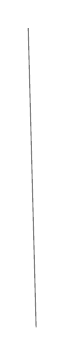
\begin{tikzpicture}\draw[gray] (0,0)--(-.1,3.8);\end{tikzpicture}}}
``\uline{Théorème}'' 8.5. En admettant lesingrédients précédents pour la cohomologie cristalline (\inserted{formule des} coefficients universels, dualité de Poincaré, théorème \unsure{de} Lefschetz \inserted{``faible''}\deleted{y compris pour les groupes de torsion}\inserted{sans négliger la torsion}), on obtient une suite exacte, relative à une variété lisse projective connexe $X\subset P_k^r$ \inserted{de dimension $n$} sur un corps parfait de car. $p>0$, et une section hyperplane (ou par une hypersurface, \inserted{de degré $d\geq1$} cela s'y ramène \ldots) $Y$ lisse de dimension $n-1$:
\deleted{\diagram{\unsure{$(8.5.1)$\quad\begin{tikzcd}[ampersand replacement=\&,column sep=small]
0\arrow[r]\&(\operatorname{Ker}v)\arrow[r]\&(\operatorname{Coker}v)
\end{tikzcd}}}
\[
(E(Y)\otimes_W k)_{\mathrm{SS}}\qquad\operatorname{Coker}v_{\mathrm{DR}}
\]}

\mspage{5}

\scanpage{7}
\margin{\figure{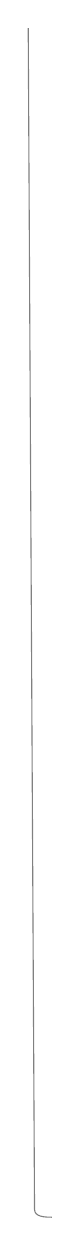
\begin{tikzpicture}\draw[gray] (0,15)--(.08,0) to[out=-90,in=180] (.3,-.1);\end{tikzpicture}}}
\diagram{$(8.5.1)$\quad\begin{tikzcd}[ampersand replacement=\&,column sep=small,row sep=large]
0\arrow[r]\&\operatorname{Ker}v\arrow[r,"\inserted{w}"]\&\deleted{\unsure{\operatorname{Coker}w}}\inserted{\text{\figure{\begin{tikzpicture}[baseline=(n.base)]\node[draw,ellipse] (n) {$({}_p\operatorname{Tors}^n(X))_{\mathrm{ss}}$};\end{tikzpicture}}}}\arrow[r]\&(E(Y)\otimes_W k)_{\mathrm{SS}}\arrow[r,"\inserted{\varphi}"]\&\unsure{E(Y,\underline O_Y)_{\mathrm{SS}}}\arrow[r]\arrow[d,phantom,"\rotatebox{90}{$=$}"]\&\inserted{0}\deleted{\unsure{\operatorname{Ker}w\longrightarrow0}}\\
\&\&\&\&\inserted{\operatorname{Coker}v}\&
\end{tikzcd},}
où on désigne par $v$ l'homomorphisme de restriction
\[
(8.5.2)\qquad v:H^{n-1}(X,\underline O_X)_{\mathrm{SS}}\longrightarrow H^{n-1}(Y,\underline O_Y)_{\mathrm{SS}},
\]
(en particulier $\operatorname{Coker}v$ est la ``cohomologie évanescente cohérente'' $E(Y,\underline O_Y)$), \deleted{et par $w$ l'homomorphisme
\[
(8.5.3)\qquad w:(\operatorname{Tors}^{n-1}(X)\otimes_W k)_{\mathrm{SS}}\xrightarrow{\inserted{u''_2}}(\operatorname{Tors}^{n+1}(X)\otimes_W k)_{\mathrm{SS}}
\]
induit par l'homomorphisme $H^{\unsure{n-1|n+1}}(X)\to H^{n+1}(X)$, \deleted{\unsure{cup}}défini par le cup-produit avec la classe de polarisation \inserted{$d\unsure{\xi|\zeta}$} sur $X$.}
\margin{\figure{\begin{tikzpicture}\node[draw,ellipse] {\unsure{Faux}};\end{tikzpicture}}}
\margin{\unsure{$K_g$} \unsure{fait donc} \illegible{4} \unsure{$V$} \illegible{2} \unsure{nul} sur la}
Enfin, pour utiliser cette suite exacte (8.5.1), on tiendra compte du fait que
\[
(8.5.4)\qquad E(Y)\overset{\mathrm{dfn}}=\operatorname{Coker}(H^{n-1}(X)\to H^{n-1}(Y))\quad\deleted{\unsure{est}}
\]
est un $W$-module libre \uline{sans torsion}; en particulier, si $k$ est un corps fini, le rang de $(E(Y)\otimes_W k)_{\mathrm{SS}}$ est égal au nombre des valeurs propres de Frobenius géométrique relatif à $k$ opérant sur $E^{n-1}(\unsure{Y|X})$ (la cohomologie cristalline évanescente de $Y$; ou ce qui revient au même, la cohomologie $\ell$-adique pour n'importe quel $\ell\ne p$ -- sous réserve de l'algébricité de l'opération $\Lambda$ sur lescohomologies cristallines et $\ell$-adiques) \uline{qui sont des unités $p$-adiques}; les valeurs propres en question, réduites \unsure{modulo} $p$, sont égales aux valeurspropres du frobenius $p$-linéaire (relatif \unsure{au} corps de base fini $k$) opérant sur le terme $E(Y)\otimes_W k$ de (8.5.1), ou si on préfère, en termes de l'interprétation 8.4.2, aux valeurs propres du \inserted{l'inverse du} générateur de frobenius de $G=\operatorname{Gal}(\bar k/k)$ opérant sur le vectoriel de dimension finie sur $\underline F_p$ correspondant.

Notons d'autre part l'égalité suivante déduite de (8.5.1):
\[
\begin{aligned}
(8.5.5)\quad\dim(E(Y)\otimes_W k)_{\mathrm{SS}}={}&\dim E(Y,\underline O_Y)_{\mathrm{SS}}\deleted{\unsure{-\dim\operatorname{Ker}w}}\\
&+(\dim\deleted{\operatorname{Coker}w}\inserted{({}_p\operatorname{Tors}^n(X))_{\mathrm{ss}}}-\dim\operatorname{Ker}v),\quad\unsure{*}
\end{aligned}
\]
où le terme entre parenthèses du deuxième membre est $\geq0$, de sorte \unsure{qu'on}

\mspage{6}

\scanpage{8}
a aussi l'inégalité suivante (résultant déjà de la suite exacte des
trois derniers termes de (8.5.1)):
\[
(8.5.6)\qquad \dim(E(Y)\otimes_W k)_{\mathrm{SS}}\geq\dim E(Y,\underline O_Y)_{\mathrm{SS}}\deleted{+\dim\operatorname{Ker}w}
\]
\deleted{\[\dim E(Y,\underline O_Y)_{\mathrm{SS}}-t^{n-1}(X,p),\]
où $t^i(X,p)$ désigne le nombre de \inserted{$p$-}coefficients de torsion de $X$ (défini
via la cohomologie cristalline de $X$ en dimension $i$).}

\uline{Remarques} 8.5.7. Je pense que l'homomorphisme $v$ de (8.5.2) est
injectif\deleted{\unsure{,}} (ce qui simplifie en conséquence (8.5.1) et (8.5.5), puisque
on aurait $\operatorname{Ker}v=0$); c'est vrai en tous cas si \inserted{$n=2$, ou si}
$Y$ est \deleted{de degré assez}
une section par une hypersurface de degré $d$ assez grand pour qu'on ait
\[H^{n-1}(X,\underline O_X(-d))=0.\]

\deleted{D'autre part, on peut si on veut dans 8.5.5 bloquer ensemble les \unsure{deux}
termes $\dim\operatorname{Coker}w-\dim\operatorname{Ker}w$, \deleted{car on aura comme}\inserted{pour trouver} la différence des
rangs \deleted{$\dim\operatorname{Coker}w-\dim\operatorname{Ker}w$} des deux membres de (8.5.3).}

8.5.8. Lorsque \deleted{dans} l'on applique (8.5.5) en prenant pour $Y$ une secti-
on de $X$ avec une hypersurface de degré $d$ ``assez générale'' (de telle
façon que le rang semi-simple de $E(Y,\underline O_Y)$ ait la valeur maxima), alors
on trouve qu'aux terme $-\dim\operatorname{Ker}v$ près (sans doute toujours nul, cf.
8.5.\unsure{7}) le deuxième membre est \uline{indépendant du choix} \deleted{de} \uline{particulier de $Y$}.
Cette remarque s'applique en particulier (8.5.7) si $d$ est assez grand.
On en conclut que si $k$ est fini, \deleted{\illegible{1}} on peut trouver un ouvert \inserted{$U_d$} de l'es\unsure{pa}-
ce projectif des hypersurfaces de degré $d$, tel que pour \deleted{tout}\inserted{un} point \inserted{\unsure{variable}} de $U$
à coefficients dans une extension finie $k'$ de $k$, le nombre de valeurs
propres de Frobenius opérant sur la cohomologie évanescente de $Y_{\bar k}$ et
qui sont des unités $p$-adiques soit constant. \deleted{Mieux, quitte à agrandir
un peu $k$, de sorte que les valeurs propres de $\operatorname{Frob}_k$} Nous désirons mon-
\mspage{7}

\scanpage{9}
rer que pour $d$ assez grand, ce nombre est non nul (ce qui impliquera \deleted{\unsure{al}}
alors\deleted{,} -- et est sans doute équivalent -- que le motif $E(Y)$ pour tous
ces $Y$ est de \uline{niveau} maximum $n-1$, ou encore que le motif $E(Y)$ pour $Y$
générique est de niveau $n-1$). Sous la forme de (8.5.6)\deleted{\unsure{*}}, on voit que
ceci est assuré dès que l'on sait que
\[
\dim E(Y,\underline O_Y)_{\mathrm{SS}}\deleted{\unsure{\longrightarrow+\infty}}\inserted{>0}\qquad\text{pour}\quad d\longrightarrow+\infty,
\]
où le dim est pris bien entendu avec sa valeur générique.
\deleted{\unsure{On sait en effet} (cf n° \unsure{7}) que $\dim\unsure{E(Y,\underline O_Y)_{\mathrm{ss}}}>\unsure{\rho|0}$ pour $d$ grand, et que $\varphi\ne0$ \unsure{pour $d$ grand} (avec \unsure{$E(Y)$} \unsure{de niveau} $\unsure{n}-1$) dès que l'on sait que $\dim(\operatorname{Tors}^{\unsure{n+1|n-1}}(X)\unsure{\otimes}k)_{\mathrm{ss}}<\unsure{\rho|p}-1$.}
\margin{Or cela est établi au n° 7}

8.5.9. Le corps de base $k$ étant à nouveau quelconque (même pas nécessai-
rement parfait), désignons, pour un degré $d$ donné, par $U_d$ l'ouvert de
l'espace projectif des hypersurfaces de degré $d$ dans $P^r_k$, formé des
hypersurfaces dont l'intersection avec $X$ est \deleted{non singulière}\inserted{lisse} de \unsure{dimension}
$n-1$, et telles que $E(Y,\underline O_Y)_{\mathrm{SS}}$ soit de rang maximum. Alors les suites
exactes (8.5.1), pour les $Y$ provenant de points de $U_d$, proviennent d'u\unsure{ne}
suite exacte de Modules localement libres \inserted{sur $U_d$} à opération $p$-linéaire semi-
simple, ou de façon équivalente (cf 8.4.2) à une suite exacte de systè-
mes locaux \inserted{de vectoriels sur $\underline F_p$} sur $U_d$ pour la topologie étale, \deleted{formés} ou enfin, une fois
choisi un point géométrique de $U_d$ (par exemple via une clôture \unsure{séparable}
du point générique) une suite exacte de représentations \inserted{de $G=\pi_1(U_d)$} dans des vectori-
els de dimension finie sur $\underline F_p$. \deleted{On} On trouve un homomorphisme \inserted{$\varphi$} du
système local défini par les $E(Y)\otimes_W k'$ \deleted{dans}\inserted{\uline{sur}} celui défini par les
$E(Y,\underline O_Y)$, dont les noyau \deleted{et le conoyau sont des}\inserted{est un} système\deleted{s} loca\deleted{ux}\inserted{l} \uline{\unsure{constant}}
(i.e. provenant du corps de base $k$). Lorsque $k$ est fini, on peut suppo-
ser, quitte à passer à une extension finie de $k$, que les valeurs propres
du frobenius relatif à $k$ opérant sur ce\deleted{s} dernier\deleted{s} \deleted{\unsure{deux}} sont toutes
égales à $1$ (il suffit que les valeurs propres de frobenius relatif à $k$
opérant sur \deleted{les} $H^{n\deleted{\unsure{-1}}}(X,\underline O_X)_{\mathrm{SS}}$ \deleted{et sur les deux membres de (8.5.3)} soient
\mspage{8}

\scanpage{10}
toutes égales à $1$). On trouve alors une description complète de la
variation des valeurs propres mod $p$ de frobenius opérant sur $E(Y)$, pour
$Y$ variable avec un point de $U_d$, en termes essentiellement de la seule
représentation de $G$ dans un vectoriel de dimension finie sur $\underline F_p$, corres-
pondant aux $E(Y,\underline O_Y)_{\mathrm{SS}}$ (donc essentiellement aux ``matrices de Hasse-Witt\unsure{''}
des $Y$ en dimension critique), -- et bien entendu de la distribution des
\deleted{frobenius} éléments de frobenius dans $G$ en termes d'un point variable de
$U_d$.

8.5.10. L'homomorphisme fondamental $\phi$ de (8.5.1) est \deleted{surjectif}
\deleted{(resp.} injectif\deleted{)} \inserted{donc bijectif} si et seulement si $w$ dans 8.5.\unsure{1} est \deleted{injectif}
\deleted{(resp. si $w$ est} surjectif, \inserted{et, \unsure{il l'est si} $({}_p\operatorname{Tors}^n(X))_{\mathrm{ss}}=0$,} le seulement si étant vrai sous la réserve
$\operatorname{Ker}v=0$ de 8.5.7); il suffit en particulier pour ceci que $X$ n'ait pas
de $p$-torsion en \deleted{caractéristique} dimension $n\deleted{\unsure{-1}}$ \deleted{(resp. en dimension \unsure{$n$}\deleted{\unsure{ou}}
$n+1$)} ou ce qui revient au même par dualité, en dimension $n\unsure{+1}$). Lorsque $X$
se \deleted{Je pense que même si} relève (avec sa polarisation) en caractéristi-
que nulle, ce\deleted{s}\inserted{tte} condition\deleted{s} \deleted{\unsure{resp.}}\inserted{suffisante\deleted{s}} doi\deleted{vent}\inserted{t} aussi pouvoir s'exprimer (une
fois qu'on disposera de fondements satisfaisants pour la cohomologie
cristalline) par \unsure{l\deleted{es}\inserted{a}} condition\deleted{s} analogue\deleted{s} sur la \inserted{torsion de} cohomologie $p$-\uline{adique}
de la variété relevée (sur un corps algébriquement clos, ou si on veut,
sur le corps des complexes $\ldots$): \deleted{on réécrit (8.5.3) en termes de
$p$-torsion de cette variété tensorisée par $\underline Z/p\underline Z$ (mais en supprimant les
indices ss, qui n'ont plus de sens), et on demande que $w_p$ ainsi défini
soit surjectif resp. injectif $\ldots\unsure{.}$

Je pense que même si $n=\dim X=2$, il peut arriver que $\phi$ ne soit
pas surjectif, \deleted{i.e.} qu'on ne peut pas dans l'inégalité (8.5.6) supprimer
le terme correctif $\dim\operatorname{Ker}w$ ou $t^{n-1}(X,p)$. En effet\deleted{\unsure{,}}, si $X$ est une}
\mspage{9}

\scanpage{11}
\deleted{Noter d'autre part qu'on a équivalence entre les conditions
suivantes:

a) L'homomorphisme $\phi$ est surjectif (resp. injectif) pour tout $d$
et tout point $s\in U_d$ (définissant un $Y$ correspondant).

b) Même condition, mais avec \uline{un} $d$ fixé multiple de $p$, et tel
que \deleted{\unsure{si}} l'on ait $\operatorname{Ker}v=0$ (condition sans doute automatiquement \unsure{vérifiée}
(8.5.7)).

c) $(\operatorname{Tors}^{n-1}(X)\otimes_W k)_{\mathrm{SS}}=0$ (resp. $(\operatorname{Tors}^{\unsure{n+1}}(X)\otimes_W k)_{\mathrm{SS}}=0$).}

\inserted{8.5.\unsure{11}.} Il serait intéressant de donner des exemples où \deleted{ces conditions ne sont pas
satisfaites.}\inserted{$\phi$ n'est pas bijectif}
\deleted{Noter que la condition non respée est toujours satisfaite
si $n=2$ ($X$ une surface). Dans le cas général,} on a l'inégalité
\[
\inserted{(8.5.1\unsure{0|1}.1)}\quad
\dim_k H^{n-1}(X,\underline O)_{\mathrm{SS}}=\dim_{\underline F_p}H^{n-1}(\bar X,\underline Z/p\underline Z)\geq\dim((H^{\inserted{n-1}}(X)/\operatorname{Tors}^{n-1}(X))\otimes k)_{\mathrm{SS}}
\]
(grâce à 8.1.2 et 8.4.3 ; en fait cela marche en toute dimension $i$, pas
seulement $i=n-1$), et dire que $\phi$ est bijectif signifie que l'inégalité
précédente est une égalité. L'exemple de Serre au symposium de Mexico
fournit un $X$ (quotient d'une intersection complète par un groupe $G=\underline Z/p\underline Z$
opérant sans points fixes) pour lequel on a $H^1(X)=0$, mais $H^1(X,\underline Z/p\underline Z)\simeq\underline Z/$
Quitte à couper avec des hyperplans, on trouve le même exemple avec
$\dim X=2$. Pour cet exemple, \deleted{(8.5.11.1) n'est pas une égalité, et
par suite,} d'après \deleted{ce qui précède,}\inserted{8.1.2. on aura}
\diagram{\begin{tikzcd}[ampersand replacement=\&,column sep=small,row sep=small]
 \& \inserted{H^1(X,\underline O)_{\mathrm{ss}}} \arrow[d,equal] \& \\
({}_{\inserted{p}}\operatorname{Tors}^{\unsure{2}}(X)\deleted{\unsure{\otimes k}})_{\mathrm{SS}} \arrow[r,phantom,"\simeq" description] \& H^1(X,\underline Z/p\underline Z)\otimes k \arrow[r,phantom,"=" description] \& \operatorname{Ker}\varphi
\end{tikzcd}}
(quel que soit $d$ et la section $Y$ de $X$ de degré $d$, permettant de définir
$\phi$), qui est non nul, donc $\phi$ n'est pas injectif. \deleted{Si maintenant $Z$ est
un schéma lisse projectif sur $k$ de dimension $n-2$ ($n$ donné $\geq\unsure{4}$), à cohomo-
logie cristalline sans torsion \inserted{et $(H^{n-4}(Z)\otimes k)_{\mathrm{SS}}\ne0$} (par exemple $P^{n-2}_k$ \inserted{si $n$ pair $\ldots$}), alors, posant
$X'=X\times Z$, on voit (sous réserve de la \uline{formule de Kunneth} en cohomologie
cristalline) que $(\operatorname{Tors}^{n-1}(X')\otimes k)_{\mathrm{SS}}$ \deleted{vient comme facteur direct} est non nul,
ce qui fournit des exemples où $\phi$ n'est pas surjectif, pour tout $n\geq4$.
Il y a sans doute aussi des exemples avec $n=3$, en cherchant bien $\ldots$.}
\mspage{10}

\scanpage{12}
8.6. La suite exacte (8.5.9) de systèmes locaux sur $U_d$ correspondant
aux suites exactes (8.5.1) met en évidence que le\deleted{s} systèmes loca\deleted{ux}\inserted{l} \unsure{corres}\inserted{pondant aux}
\deleted{des} $(E(Y)\otimes_W k)_{\mathrm{SS}}$ \deleted{et aux $E(Y,\underline O_Y)_{\mathrm{SS}}$ ont}\inserted{a} en plus d'un sous-système \deleted{resp.
d'un système quotient}\inserted{du premier} de nature essentiellement triviale (car provenant
du corps de base, donc constant du point de vue géométrique) \deleted{une}\inserted{un} \unsure{composant}
\deleted{commun $\operatorname{Coim}\phi=\operatorname{Im}\phi$}\inserted{$E(Y,\underline O_Y)_{\mathrm{ss}}$}, dont on s'attend qu'il donne lieu à une représen-
tation tout à fait non triviale de $G$ (NB si on n'aime pas les groupes
fondamentaux généraux et les systèmes locaux, on peut tout interpréter
en termes de la suite exacte 8.5.1 correspondant au \uline{point générique} $s$ de
l'espace des hypersurfaces de degré $d$ dans $P^r_k$, et remplacer $G$ par le
groupe $\operatorname{Gal}(\overline{k(s)}/k(s))$, -- mais on perd alors les frobenius $\ldots$). On aime-
rait pouvoir préciser ce point. \inserted{(Si $n\geq2$, cette représentation est-elle \uline{irréductible}, \unsure{au moins} \unsure{?})} Par exemple, l'image du groupe \unsure{fondamental}
\inserted{$G$} dans $\operatorname{Aut}(V)$ ($V$ étant le \deleted{\unsure{corps}} vectoriel de dimension finie sur $\underline F_p$ où
s'effectue la représentation envisagée de $G$) est-elle égale à $\operatorname{Aut}(V)$ tout
entier ? \inserted{(Ce n'est pas \deleted{\unsure{exclu} \illegible{1}} lorsque $X=P_k^{\unsure{r=1}}$, cas qu'on peut traiter directement) dès que la condition \unsure{ci-dessus est remplie}}
\deleted{Si oui,} alors dès que \inserted{\unsure{l'on a}} $\dim V\geq2$ (ce qui est sans doute \unsure{vrai}
dès que $d$ est assez grand, $\dim V$ tendant vers $\infty$ avec $d$, cf. 8.5.8),
tout élément de $\underline F_p$ est trace d'un élément de $G$ opérant sur $V$. De ceci,
\inserted{de la ``formule de Woodshole'' \deleted{\unsure{via le|on le} \illegible{4}}}
et du théorème de Čebotareff, on déduirait alors,\deleted{\unsure{,}} si le corps $k$ est fini
qu'on peut, pour n'importe quel ouvert non vide $U$ de l'espace des hyper-
surfaces de degré $d$ dans $P^r_k$ ($d$ étant choisi comme dessus) trouver un
point \deleted{de} $s$ de $U$ à coefficients dans une extension finie $k'$ de $k$, définis-
sant une section $Y$ telle que $\operatorname{card}Y(k')$ soit congru mod $p$ à un élément
de $\underline F_p$ donné à l'avance. Au moment d'écrire ces lignes, et malgré l'assis-
tance de gens compétents comme Katz, il ne semble pas qu'un résultat de
cette nature soit prouvé\deleted{,}\inserted{(} même si $X=P^{2\inserted{=r}}$ i.e. pour des courbes planes \inserted{$Y$} de
grand degré\inserted{)}. \deleted{Ce résultat serait déjà bien intéressant, car il implique-
rait déjà une réponse affirmative à la conjecture du n°6 sur le niveau
de la cohomologie évanescente (dont il est question aussi dans 8.5.8).}
\mspage{11}

\cotefile{100}
\scanpage{1}
\figure{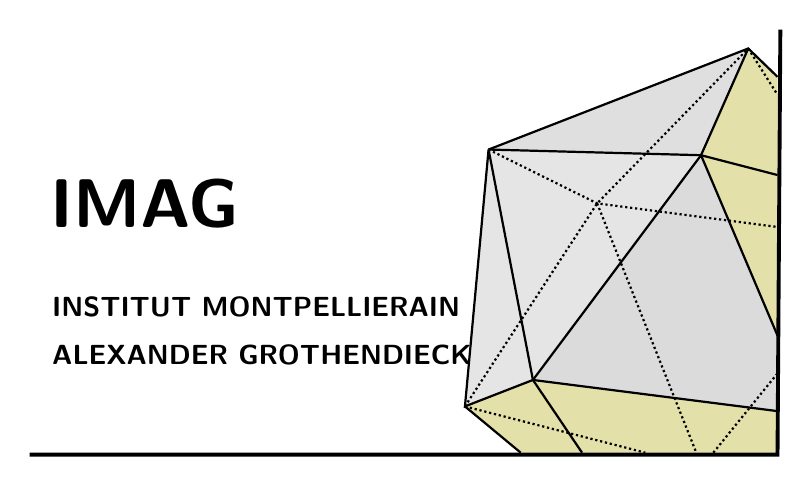
\begin{tikzpicture}[x=.012cm,y=-.012cm,line width=.8pt]
\node[anchor=west,font=\sffamily\bfseries\Huge] at (20,195) {IMAG};
\node[anchor=west,font=\sffamily\bfseries] at (22,305) {INSTITUT MONTPELLIERAIN};
\node[anchor=west,font=\sffamily\bfseries] at (22,355) {ALEXANDER GROTHENDIECK};
\fill[gray!25] (495,138)--(770,31)--(720,144)--cycle;
\fill[gray!20] (495,138)--(720,144)--(542,382)--(470,410)--cycle;
\fill[gray!28] (720,144)--(801,335)--(801,415)--(542,382)--cycle;
\fill[olive!25] (770,31)--(801,61)--(801,335)--(720,144)--cycle;
\fill[olive!25] (470,410)--(542,382)--(801,415)--(801,459)--(529,459)--cycle;
\draw (495,138)--(770,31)--(801,61);
\draw (495,138)--(720,144)--(770,31);
\draw (720,144)--(801,165);
\draw (495,138)--(470,410)--(542,382)--(495,138);
\draw (542,382)--(720,144)--(801,335);
\draw (470,410)--(529,459);
\draw (542,382)--(594,459);
\draw (542,382)--(801,415);
\draw[densely dotted] (495,138)--(610,195)--(801,220);
\draw[densely dotted] (470,410)--(610,195)--(770,31);
\draw[densely dotted] (610,195)--(715,459);
\draw[densely dotted] (470,410)--(661,459);
\draw[densely dotted] (733,459)--(801,375);
\draw[densely dotted] (770,31)--(801,80);
\draw[line width=1.4pt] (9,461)--(801,461)--(804,11);
\end{tikzpicture}}

\scanpage{2}
Bonne \unsure{réduction}
et \unsure{gpes|groupes} $p$-divisibles
\mspage{1}

\scanpage{3}
\figure{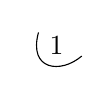
\begin{tikzpicture}[x=1cm,y=1cm]\node at (0,0) {\mspage{1}};\draw (-.23,.17) .. controls (-.36,-.31) and (.05,-.36) .. (.32,-.13);\end{tikzpicture}}
\uline{Théorème} $S$ schéma loc. noeth, $U$ ouvert, $T$ fermé complémentaire,
$p$ \unsure{ent} premier, tel que $\forall t\in T$, $\operatorname{car}k(t)=p$. Considérons la
catégorie $C$ des schémas abéliens \inserted{$A$} sur $S$, et la catégorie $C'$ des
couples $(A_U,M,\varphi)$, où $A_U$ est un schéma abélien sur $U$, $M$
un \unsure{grpe|groupe} $p$-divisible sur $S$, et $\varphi:M|U\longrightarrow T_p(A_U)$. Soit
\[F:C\longrightarrow C'\]
le foncteur
\[F(A)=(A\times_S U,T_p(A),\operatorname{id}_{T_p(A)|U}).\]
Alors:

1) Supposons que $U$ rencontre ttes composantes connexes
de $S$. \inserted{(\unsure{p.ex.} $U$ dense dans $S$, i.e. $\operatorname{prof\,et}_T(S)\geq1$).} Alors le foncteur $F$ est pleinement fidèle.

2) Supposons que \deleted{$U$ soit dense dans $S$, et que}
\inserted{a) $\exists$ morphisme fini surjectif $S'\longrightarrow S$, avec $S'$ géom. unibranche (\unsure{p.ex. la normalisée} de $S$ est finie sur $S$, si $S$ local).}
\deleted{\inserted{b)} pour tout $t\in T$, si $S'$ est le localisé strict de $S$ en $t$,
\inserted{($\bar t$ son point fermé)} et $S'_1$ et $S'_2$ deux composantes irréductibles de $S'$, on ait
\[S'_1\cap S'_2\ne\{\bar t\}.\]
(NB. Cette condition équivaut aussi à celle-ci:
\deleted{\unsure{dans un} \illegible{2}} l'image inverse $U''$ de $U$ dans $S''=S'\times_S S'$
\deleted{équivalence de catégories} \unsure{est dense dans} $S''$. \unsure{Et $U$ est} \unsure{un} \illegible{1} \deleted{\unsure{strict}} \unsure{géom. connexe}
\unsure{en un point de} $T$) Alors \deleted{b) Posant}}
\inserted{b) On a $\operatorname{prof\,et}_T(S)\geq2$ \unsure{\S}.}
Alors $F$ est \deleted{pleinement fidèle}\inserted{une équivalence des catégories}.
\margin{\figure{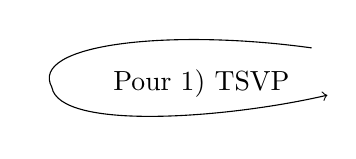
\begin{tikzpicture}[x=1cm,y=1cm]
\node at (1.7,0) {Pour 1) TSVP};
\draw[->] (3.1,.45) .. controls (1.3,.7) and (-.5,.5) .. (-.2,-.05) .. controls (-.1,-.6) and (2,-.45) .. (3.3,-.15);
\end{tikzpicture}}}

\margin{$\S$ Soit, avec les notations de a), $S''=S'\times_S S'$, $S'''=S'\times_S S'\times_S S'$. Considérons
l'ensemble simplicial
\diagram{\begin{tikzcd}[ampersand replacement=\&,column sep=large,row sep=small]
\inserted{L_0} \arrow[d,phantom,"\unsure{\Vert}" description] \& \inserted{L_1} \arrow[d,phantom,"\unsure{\Vert}" description] \& \inserted{L_2} \arrow[d,phantom,"\unsure{\Vert}" description] \\
\pi_0(S') \& \pi_0(S'') \arrow[l,shift left=.6ex] \arrow[l,shift right=.6ex] \& \pi_0(S''') \arrow[l,shift left=1ex] \arrow[l] \arrow[l,shift right=1ex]
\end{tikzcd}}, \deleted{\unsure{les}} et \deleted{soit}
soit
\diagram{\begin{tikzcd}[ampersand replacement=\&]K_0 \& K_1 \arrow[l,shift left=.6ex] \arrow[l,shift right=.6ex] \& K_2 \arrow[l,shift left=1ex] \arrow[l] \arrow[l,shift right=1ex]\end{tikzcd}}
le ss-ensemble simplicial formé avec
les composantes connexes dont l'image dans $S$ rencontre $U$.
Supposons\unsure{:} \unsure{que:} \deleted{pour tout}\inserted{b')} la plus petite partie de $L_1$
contenant $K_1$ et stable par ``troisième face'' soit $L_1$ (c'est
ce qui est assuré par la condition b)). Alors $F$ est \deleted{\unsure{pl. fid.}}
\inserted{une} équivalence de catégories $\ldots\ldots$.}
\mspage{2}

\scanpage{4}
\figure{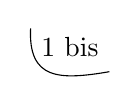
\begin{tikzpicture}[x=1cm,y=1cm]\node at (0,0) {\mspage{1 bis}};\draw[thin] (-.5,.23) .. controls (-.53,-.42) and (-.14,-.43) .. (.5,-.32);\end{tikzpicture}}
\margin{\figure{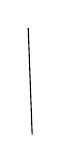
\begin{tikzpicture}\draw (0,0)--(.05,-1.35);\end{tikzpicture}}}\uline{Lemme} $A,B$ schémas abéliens sur $S$ loc. noeth, $u_\ell:T_\ell(A)\longrightarrow T_\ell(B)$.
Alors $\exists$ \uline{sous-schéma fermé} $T$ de $S$ tel que, pour tout $S'/S$ on
\inserted{ait:} $u_{\ell S'}$ provient de $u:A_{S'}\unsure{\mathbin{-}|\longrightarrow}B_{S'}$ ssi $S'$ se factorise par $T$.

Cf Inventiones 1.2 (\unsure{ou|où} démonstration \unsure{cristalline}).

\deleted{\uline{Cor} Supposons que $\forall s\in\unsure{\operatorname{Ass}^0_S|\operatorname{Ass}_S}$ \unsure{l'une des} hyp. suiv\unsure{.}
\deleted{\unsure{Ht}} \unsure{de la} \illegible{1}}
\margin{\figure{\begin{tikzpicture}\draw[thin] (0,0)--(0,-.35);\draw (0,-.5)--(.04,-1.2);\end{tikzpicture}}}\uline{Complément} De plus, pour $\forall t\in T$
tel que $\operatorname{car}k(t)=\ell$, $T$ \unsure{comprend|contient} un voisinage ouvert
\unsure{immédiat} de $t$.

\uline{Corollaire} Supposons que l'ouvert $U\subset S$ soit tel que

a) tte comp. conn. de $S$ rencontre $U$

b) $t\in S-U\Longrightarrow\operatorname{car}k(t)=\ell$.

c) $u_\ell|U$ provient de $u_U:A|U\unsure{\mathbin{-}|\longrightarrow}B|U$

Alors \deleted{\unsure{$A$}} $u_\ell$ provient de $u:A\longrightarrow B$.
\margin{donc $\Longrightarrow U\ne\varnothing$.}

\deleted{En effet, on peut supposer $S$ connexe, \inserted{Alors} \deleted{\unsure{$T$ est} \illegible{1}} \unsure{le} \illegible{2}
réunion de composantes irréductibles [dont le générique $t\in\unsure{T\cap U}$
et $t\in T\cap(S-U)$] \inserted{grâce à b)}, \deleted{\unsure{de} si $S_i$ \unsure{avait} \unsure{ou} $\unsure{\not\subset}S$
on aurait une comp. $S_i$ de $S$ telle que}
\inserted{Comme $T\ne\varnothing$, il suffit de} prouver que tte comp. irréd. de $S$ qui rencontre
$T$ est $\subset T$. Or si $S_i\cap U=\varnothing$ alors, \inserted{comme $T\supset\bar U$,} \unsure{on} aussi grâce au complément \inserted{et ailleurs}.
Donc $T\supset S_{red}$. \unsure{Alors}
Mais $T$ est \deleted{\unsure{ind}} ouvert}
$T$ est ouvert induit sur
$U$ par hyp. \inserted{c)}, et en les pts de $(S-U)\cap T$ grâce au
complément et de b). Donc $\unsure{T|\bar T}$ est un \inserted{sous-schéma} ouvert,
et comme il est fermé, c'est une réunion de
comp. connexes. Par \unsure{a)} on a donc $T=S$,
cqfd.
\mspage{3}

\scanpage{5}
\mspage{2)}
\figure{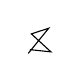
\begin{tikzpicture}[scale=.4]\draw (0,0)--(.65,.8)--(.1,.62)--(.72,.05)--(.05,.12);\end{tikzpicture}}
\[
T\subset S\supset U=S-T
\]
\margin{\figure{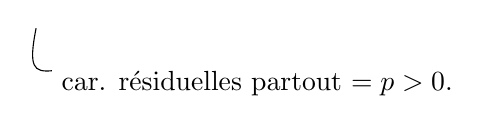
\begin{tikzpicture}\node[anchor=west] at (.2,0) {car. résiduelles partout $=p>0$.};\draw (0,.7) .. controls (-.1,.2) and (-.03,.14) .. (.2,.16);\end{tikzpicture}}}
\margin{\unsure{3.}}
\[
A\longmapsto (A_U,T_p^{\unsure{f|p}}(A),\varphi)
\]
schémas abéliens sur $S$ \qquad triples $(A_U,M,\varphi)$
\[
\begin{aligned}
&A_U\quad\text{schém. abélien sur }U\\
&M\quad\text{\unsure{grpe} $p$-div sur }T\\
&\varphi:T_p^{\unsure{f|p}}(A_U)\simeq M.
\end{aligned}
\]
\margin{$S$ noethérien, $U$ \deleted{dense} \deleted{\unsure{schémati.}} \deleted{\uline{\unsure{schématiquement}}} dense et $S-U$ à car. $p$.}
\margin{\figure{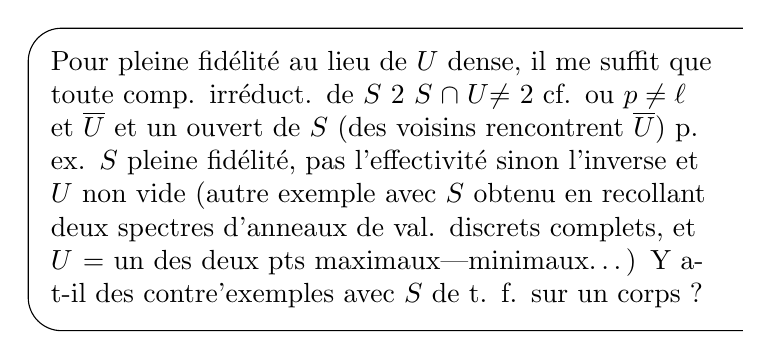
\begin{tikzpicture}\node[inner sep=8pt,text width=8.5cm] (n) {Pour pleine fidélité au lieu de $U$ dense, il me \unsure{suffit que} \deleted{\unsure{toute} comp. \unsure{irréduct.}} \deleted{\unsure{de $S$} \illegible{2} $\unsure{S}\cap U\unsure{\ne}\varnothing$ \illegible{2}} \deleted{\unsure{cf. ou} $\unsure{p\ne\ell}$} \deleted{et $\overline U$ \unsure{et un ouvert} de $S$ (\unsure{des voisins} \unsure{rencontrent} $\overline U$)} p. ex. $S$ \deleted{\unsure{pleine fidélité}, \unsure{pas l'effectivité}} \unsure{sinon l'inverse et $U$ non vide} (autre exemple \unsure{avec} \unsure{$S$} obtenu en \unsure{recollant} deux spectres d'anneaux de val. discrets complets, et $U=$ un des deux pts \unsure{maximaux|minimaux}\dots) Y a-t-il des contre'exemples avec $S$ de \unsure{t. f.} sur un \unsure{corps} ?};\draw[rounded corners=12pt] (n.north east)--(n.north west)--(n.south west)--(n.south east);\end{tikzpicture}}}

1) \uline{Foncteur pleinement fidèle}

fidèle bien connu, car $A\mathbin{-}T_p^{\unsure{f|p}}(A)$ est fidèle.

``pl.'' fidèle: il faut prouver que si $u_p:T_p^{\unsure{f|p}}(A)\mathbin{-}T_p^{\unsure{f|p}}(B)$ est algébrique sur $U$, il l'est sur $S$. Si $U$ est sch. dense dans $S$, cela résulte de $[\ ]$ 1.2. Dans le cas général, soit $X_0$ l'adhérence schématique de $U$ dans $X$.
Alors on dispose d'un hom $\varphi_0:A_{X_0}\to B_{X_0}$, \deleted{\unsure{On voit}} \inserted{compatible avec $u_p$.}

\deleted{Soit $\unsure{I}$ l'idéal qui définit $X_0$ en $X$, \unsure{est nilpotent} \unsure{et} \unsure{s'annule} sur $T$. Alors la \unsure{th.rie} de Serre-Tate implique que l'on peut prolonger la restriction de $\unsure{u_0}$ à $T_0^{\deleted{\unsure{\mathrm{r\acute ed}}}}$ \inserted{$=T$} (muni de la structure induite réduite) en un hom. $A_{T_n}\to B_{T_n}$, où $T_n$ est le $n$-ième voisinage infinitésimal. Se ramenant au cas $S$ affine, \inserted{$=\operatorname{Spec}\Lambda$} on trouve \deleted{\unsure{par l'\illegible{1}}} un hom $A_{\hat\Lambda}\mathbin{-}B_{\hat\Lambda}$, $\hat\Lambda=$ complété de $\Lambda$ pour la top. définie par l'idéal de $T_0$ dans $S_0$. Comme l'hom \deleted{$U\times\unsure{\operatorname{Spec}}$} $\hat\Lambda\to\operatorname{Spec}\Lambda$ est fid plat, on gagne\dots}
\inserted{en appliquant alors $[\ ]$ 1.1.}
\mspage{4}

\scanpage{6}
\mspage{-0.13-}
image of $\phi'$. Since this image is dense, there are no such $y$'s.
Therefore $\sigma[\phi^{-1}(U)]=\phi^{-1}(U)\times_U U'$, and $\phi'$ is surjective.
Therefore $\overline\omega$ is geometrically injective without restriction, and by \uline{Zariski's Main Theorem}, $\overline\omega$ is an isomorphism. \uline{QED}
\margin{!}

\uline{Remark} \uline{(5)}. The following are equivalent:

(a) $(Y,\phi)$ is a universal categorical quotient of $X$ by $G$,

(b) for all affine schemes $Y'$, and morphisms $Y'\longrightarrow Y$, if $\phi':X'\to Y'$ is the base extension, then $(Y',\phi')$ is a categorical quotient of $X'$ by $G$,

(c) there is an affine open covering $\{U_i\}$ of $Y$ such that if $\phi_i:\phi^{-1}(U_i)\longrightarrow U_i$ is the restriction of $\phi$, then $(U_i,\phi_i)$ is a universal categorical quotient of $\phi^{-1}(U_i)$ by $G$, for all $i$.

(6). In Chapter 1, we will need a criterion for $(Y,\phi)$ to be a categorical quotient which does not imply that $(Y,\phi)$ is a geometric quotient. In fact, the following 3 conditions suffice:

\[
\text{i)}\qquad\phi\circ\sigma=\phi\circ p_2,
\]
ii) $\underline o_Y$ is the subsheaf of invariants of $\phi_*(\underline o_X)$,

iii) if $W$ is an invariant closed subset of $X$, then $\phi(W)$ is closed in $Y$; if $W_i$, $i\in I$, is a set of invariant closed subsets of $X$, then:
\[
\phi\left(\bigcap_{i\in I}W_i\right)=\bigcap_{i\in I}\phi(W_i)
\]
\margin{\diagram{\begin{tikzcd}[ampersand replacement=\&,column sep=large]
R\arrow[d,shift right=.6ex,"p_1"']\arrow[d,shift left=.6ex,"p_2"] \& \\
\varphi:X\arrow[r,"\unsure{f}"'] \& Y
\end{tikzcd}}
morphism of preschemes \unsure{st.h.} $\varphi p_1=\varphi p_2$ \unsure{with} $Y$ is a quotient $X/R$ if
(i) $\underline O_Y$ is the sheaf of invariant of
\diagram{\begin{tikzcd}[ampersand replacement=\&,column sep=small]
\underline O_Y\arrow[r,dash] \& f_*(\underline O_X)\arrow[r,shift left=.6ex]\arrow[r,shift right=.6ex] \& g_*(\unsure{O_R})
\end{tikzcd}}
(ii) Any invariant open $U$ of $X$ is the inverse image of an open subset of $Y$.}
\margin{\figure{\begin{tikzpicture}\draw[thin] (0,0) .. controls (.09,-.6) and (.07,-1.05) .. (-.3,-1.65);\end{tikzpicture}}Il paraît suffisant que $\varphi$ \unsure{soit} \uline{\unsure{quasi-qct|quasi-cpt}} par \unsure{exp.}}
\mspage{5}

\scanpage{7}
\figure{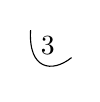
\begin{tikzpicture}[x=1cm,y=1cm]\node at (0,0) {\mspage{3}};\draw (-.22,.2) .. controls (-.25,-.3) and (.05,-.35) .. (.3,-.15);\end{tikzpicture}}
2) \uline{Foncteur ess. surjectif}
\margin{\fbox{\parbox{.6\linewidth}{\uline{Si} $S$ \uline{géom. unibranche en les points de} $S-U$ (\unsure{.}\par et si le normalisé de $S_{\mathrm{red}}$ est \unsure{fini} sur $S$.}}}
\margin{[plus gén., si, posant $S''=S'\times_S S'$, $U'=U\times_S S'$, $U''=U\times_S S''$, $U^{(\unsure{n})}$ \deleted{\unsure{rencontre}} rencontre ttes comp$^{\unsure{\mathrm{tes}}}$ connexes de $S^{(\unsure{n})}$]}
\figure{\begin{tikzpicture}[x=1cm,y=1cm]\draw[->] (0,0)--(-.45,0);\draw[->] (4.8,-2.1)..controls(4.4,-1.3)and(6,.1)..(5,0);\end{tikzpicture}}
\deleted{a) \unsure{Supposons}}
Partant de $A_U,M,\varphi$, on veut construire $A$.
\inserted{On peut supposer $S$ affine, $S=\operatorname{Spec}\Lambda$.}
\deleted{Par descente, il suffit de \unsure{traiter ce cas}.}

a) Réduction au cas $S$ réduit.

Soit $S_0=S_{\mathrm{red}}$, $A_0$ schéma abélien sur $S_0$ qui y résout le pb. Par Serre-Tate, on trouve \deleted{\unsure{des}}\inserted{\deleted{\unsure{un}}} schémas abéliens sur les $T_n$, donc un schéma \inserted{formel} abélien \inserted{$A'$} sur $S'=\unsure{\operatorname{Spec}}\hat\Lambda$. Son image inverse sur $S'_0$ est un vrai schéma abélien, \deleted{\unsure{sur $S$}} \unsure{savoir} l'image inverse de $A_0$ sur $S'_0$. Donc (réf \dots !!!) $A'$ provient d'un vrai schéma abélien $A'$ sur $S'$ [l'immersion $S'_0\mathbin{-}S'$ étant nilpotente]. Or $U\amalg S'\to S$ est fid. plat, et on trouve une donnée de descente sur $A_U\amalg A'$. Elle \unsure{devient} effective après dépt de base $S_0\hookrightarrow S$, donc elle l'était déjà avant, d'après le critère de Raynaud. On gagne !
\margin{\unsure{?}}
\margin{\diagram{\begin{tikzcd}[ampersand replacement=\&,column sep=small,row sep=small]
S_0\arrow[d] \& S'_0\arrow[l]\arrow[d]\\
S \& S'\arrow[l]
\end{tikzcd}}}

\deleted{b) Réduction au cas $S$ local, \deleted{\unsure{et de}} $T=$ point fermé.
Pour faire cette réduction, on est amené à prouver ceci: si $t$ est un pt \unsure{maximal|général} de $T$, $V$ un ouvert contenant $t$ et $U$, \deleted{et} $A_V$ un schéma abélien sur $V$ \deleted{qui \unsure{induit}} $M$ par sa restriction à $S'=\operatorname{Spec}\underline O_{S,t}$ \deleted{\unsure{vérifie}} est OK, alors $A_V$ est \deleted{\unsure{encore}} OK dans un voisinage, i.e. l'isom donné $T_p(A_{S'})\simeq M_{S'}$ se prolonge en un isom en un}
\margin{?}
\mspage{6}

\scanpage{8}
\mspage{7}
\mspage{-0.14-}
\uline{Proof}: Note first of all that $\phi$ is dominating by (ii); hence by (iii), $\phi$ is actually \uline{surjective}. Now suppose $\deleted{\phi}\inserted{\psi}:X\longrightarrow Z$ is any $S$-morphism such that $\psi\circ\sigma=\psi\circ p_2$. We proceed exactly as in the proof of Proposition 0.1: choose an affine open covering $\{V_i\}$ of $Z$. Once we show that there is an open covering $\{U_i\}$ of $Y$ such that
\figure{\begin{tikzpicture}\node[draw,ellipse,inner sep=3pt] {$\psi^{-1}(V_i)\supset\phi^{-1}(U_i)$};\end{tikzpicture}},
we can conclude the proof as in Proposition 0.1. To show this, let $W_i=X-\psi^{-1}(V_i)$. These are closed invariants subsets of $X$. Therefore, by (iii), $U_i=Y-\phi W_i$ are open; and $\phi^{-1}(U_i)\subset\psi^{-1}(V_i)$ for all $i$. Finally, $\{\psi^{-1}(V_i)\}$ cover $X$, hence $\bigcap_iW_i=\phi$, hence by (iii) $\bigcap_i\phi W_i=\phi$, hence $\{U_i\}$ cover $Y$. \uline{QED}

(7). Suppose $(Y,\phi)$ is a geometric quotient of $X$ by $G$. Notice that conditions (i), (ii), and (iii) of Definition 0.6 are preserved by any base extension $Y'\to Y$. Only the more delicate condition (iv) might (and indeed sometimes does) break down. However, if $Y'\longrightarrow Y$ is \uline{flat}, then condition (iv) is preserved. To see this, let $\psi=\phi\circ\sigma=\phi\circ p_2$. Then (iv) asserts the exactness of:
\margin{$\varphi$ quasi-compact quasi-séparé}
\diagram{\begin{tikzcd}[ampersand replacement=\&,column sep=large]
(*)\quad 0\arrow[r] \& \underline o_Y\arrow[r] \& \phi_*(\underline o_X)\arrow[r,"\sigma^*-p_2^*"] \& \psi_*(\underline o_{G\times_S X})
\end{tikzcd}}
But taking direct image sheaves commutes with \uline{flat} base extension, i.e.
\[
\begin{aligned}
\phi_*(\underline o_X)\otimes\underline o_Y&\cong\phi'_*(\underline o_X)\\
\psi_*(\underline o_{G\times_S X})\otimes\underline o_Y&=\psi'_*(\underline o_{G\times_S X}).
\end{aligned}
\]
(where $X'=X\times_Y Y'$, etc.), and the exactness of a sequence is pre-

\scanpage{9}
\deleted{voisinage ouvert $W\ni t$, induisant ce qui est donné sur $W\cap U$. En fait, \deleted{d'après le} \inserted{si on dispose du} th. de Tate \deleted{\unsure{ceci}} \unsure{par suite} en inégales caractéristiques, on pourrait prouver}

b) Cas $S$ \deleted{normal} \inserted{géom. unib.}, $A_U$ muni d'une rigidification de Jacobi. On a donc un morphisme
\margin{\deleted{$\unsure{\ell}$}}
\diagram{\begin{tikzcd}[ampersand replacement=\&]U\arrow[r] \& R\end{tikzcd}}
\margin{\figure{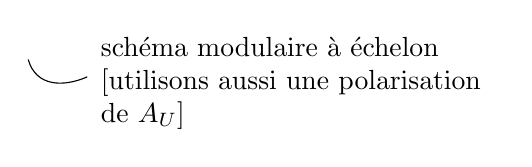
\begin{tikzpicture}\draw (0,.35) .. controls (.1,0) and (.45,0) .. (.75,.13);\node[anchor=west,text width=5cm] at (.8,.05) {schéma modulaire à \unsure{échelon} [utilisons aussi une polarisation de $A_U$]};\end{tikzpicture}}}
d'où par le \inserted{l'adhérence du} graphe un sous-schéma fermé $S'$ de $S\times R$. Le critère valuatif et le résultat de Raynaud dans le cas d'un trait \unsure{prouvent} que $S'\to S$ est propre. Il reste à prouver que c'est un isom [tout revient en effet, grâce à Tate, à prouver que $A_U$ se prolonge en $A$, quand $T_p(A_U)$ se prolonge en un $M$ -- cet $M$ étant en effet unique à iso unique près). Par le Main Theorem, on est ramené à prouver que \deleted{les pts de $S'$} \inserted{les fibres $S'_s$ sont \uline{discrètes}.} Introduisons le normalisé $S''$ de $S'$, qu'on suppose d'abord \uline{fini} sur $S'$. Alors le th. de Tate implique que le grpe $p$-divisible $T_p(A_{S''})$ \margin{\figure{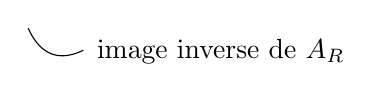
\begin{tikzpicture}\draw (0,.3) .. controls (.18,-.1) and (.45,-.1) .. (.7,.02);\node[anchor=west] at (.75,0) {image inverse de $A_R$};\end{tikzpicture}}} est l'image inverse de \deleted{$\unsure{T_p(A)}$} $M$. Donc la restriction de $A_{S''}\mid S''_s$, correspondant à un $T_p$ ``constant'', et $S''_s$ étant géom. connexe,
\margin{\diagram{\begin{tikzcd}[ampersand replacement=\&,column sep=small,row sep=small]
 \& S''\arrow[d]\arrow[r] \& U''\arrow[d,phantom,"\unsure{\Vert|\wr}"]\\
R \& S'\arrow[l]\arrow[d]\arrow[r] \& U'\arrow[d,phantom,"\unsure{\Vert|\wr}"]\\
 \& S\arrow[r] \& U
\end{tikzcd}}}
\mspage{8}

\scanpage{10}
\mspage{9}
\mspage{-0.15-}
served under flat base extension -- hence the analogous sequence $(*)'$ on $Y'$ is exact.

(8). On the other hand, consider the converse. I claim that if $Y'\longrightarrow Y$ is faithfully flat and quasi-compact, and if the extended morphism $\phi':X'\longrightarrow Y'$ makes $(Y',\phi')$ a universal categorical quotient or geometric quotient or universal geometric quotient of $X'$ by $G$, then $(Y,\phi)$ is the same type of quotient of $X$ by $G$. These asser-
tions are all simple corollaries of the general theory of descent of SGA 8.

\fbox{\S3.} We shall now look somewhat more closely at the structure of an action of a group. As above, let $G/S$ act via $\sigma$ on $X/S$.

\uline{Definition} \uline{0.8}: The action $\sigma$ is said to be

i) \uline{closed} if for all geometric points $x$ of $X$, the orbit $O(x)\subset\overline X$ is closed, (i.e. $\overline X=X\times_S\operatorname{Spec}\Omega$ if $x$ is an $\Omega$-valued point),

ii) \uline{separated} if the image of
\[
\unsure{\overline{\underline{\psi}}|\overline{\underline{\Psi}}}=(\sigma,p_2):G\times_S X\longrightarrow X\times_S X
\]
is closed,

iii) \uline{proper} if $\unsure{\overline{\underline{\psi}}|\overline{\underline{\Psi}}}$ is proper,

iv) \uline{free} if $\unsure{\overline{\underline{\psi}}|\overline{\underline{\Psi}}}$ is \figure{\begin{tikzpicture}\node[draw,ellipse,inner sep=3pt]{a closed immersion.};\end{tikzpicture}}
\inserted{\fbox{monomorphism}}
\margin{\unsure{conflits} avec \unsure{des} \unsure{terminologies} \unsure{reçues}\par dire: \uline{\unsure{proper and free}}}

Moreover, let $\mathcal S=S(1_X)$ be the stabilizer of $1_X:X\to X$ (cf. Definition 0.4). It is a sub-group pre-scheme of the group pre-scheme $G\times_S X/X$. Let $\overline\omega:\mathcal S\longrightarrow X$ be the projection and let $e_X:X\longrightarrow\mathcal S$

\scanpage{11}
on conclut (cf lemme) que $A_{S''}$ est constant.
\deleted{Il l'est en tant que variété polarisée, par fonctorialité. \unsure{Il ne reste le choix} que d'un nb fini de rigidifications de Jacobi, le $(S''_s)_{\mathrm{r\acute ed}}\to R$ se factorise par $\unsure{\operatorname{Sp}|\operatorname{Spec}}(k(s))$, donc $S''_s$ est réduit à un point. On gagne.}

Le cas où on ne suppose plus $S''$ fini sur $S'$ se traite par la méthode essentiellement de $[\ ]$ p 75--76, \uline{à condition} qu'on prouve que l'isomorphisme sur $U''\simeq U'$ entre $T_p(A'')\mid U''$ et $M_{S''}\mid U''$ se prolonge à $S''$. \deleted{Il faudrait tirer au clair cette question.} \inserted{O.K.}
\margin{?}

c) Cas $S$ \deleted{normal}. \inserted{géom. unibranche.} Choisissons un nb premier $\ell\ne p,\unsure{3}$, et soit $U'\to U$ un morphisme étale fini surjectif \deleted{\unsure{qui soit}} tel que $A_{U'}$ soit muni d'une rigidification d'ordre $\ell$.
\figure{\begin{tikzpicture}\node[draw,ellipse,inner sep=3pt] {Normalisons};\end{tikzpicture}} $S$ dans $R(U')/R(U)$, \inserted{\unsure{``} $R(S)$} d'où morphisme fini \inserted{surjectif} $S'\to S$, \inserted{\figure{\begin{tikzpicture}\node[draw,ellipse,inner sep=2pt] {prolongeant $U'\mathbin{-}U$};\end{tikzpicture}}} avec $S'$ normal intègre.
\margin{\figure{\begin{tikzpicture}\node[draw,ellipse,align=center,inner sep=3pt] {\unsure{inutile},\\\unsure{on verra} !};\end{tikzpicture}}}
Alors on peut trouver un schéma abélien $A'$ sur $S'$ qui prolonge $(A_U)\times_U U'$, avec $T_p(A')\simeq p^*(M)$.
Alors par la partie ``pl. fid'' appliquée à $S''=S'\times_S S'$, utilisant que $U''$ est dense dans $S''$ (\deleted{\unsure{par lemme}} \inserted{N.B. $S''\mathbin{-}S$ est ouvert car $S'\mathbin{-}S$ est \unsure{univers$^t$} ouvert\dots}), on trouve
\margin{\diagram{\begin{tikzcd}[ampersand replacement=\&,column sep=small,row sep=small]
U\arrow[d,phantom,"\rotatebox{90}{$\unsure{\subset}$}"] \& U'\arrow[l]\arrow[d,phantom,"\rotatebox{90}{$\unsure{\subset}$}"] \& U''\arrow[l,shift left=.6ex]\arrow[l,shift right=.6ex]\arrow[d,phantom,"\rotatebox{90}{$\unsure{\subset}$}"]\\
S \& S'\arrow[l,"p"'] \& S''\arrow[l,shift left=.6ex]\arrow[l,shift right=.6ex]
\end{tikzcd}}}
\mspage{10}

\scanpage{12}
Errata, Page 2.

$A/\mathfrak p^{(k)}$ in the expression for $E^m$. Now $A/\mathfrak p^{(k)}$ has depth 1, whether calculated as an $A$-module or a $B$-module. So it has homological dimension $r-1$ over $B$, since $B$ is regular, and hence each $\operatorname{Ext}_B^r(A/\mathfrak p^{(k)},B)=0$. Thus the $E^r$ term of the abutment is zero, so each ''

Page 43, Line 4: insert ``locally free $F$, and hence for all'' after ``for all''.

Page 46, Line 9: insert ``proper over $k$, '' before ``and''.

Page 46, Line -2: add ``[AVB 2.2 and 3.3]'' at end of line.

Page 50, Line -6: replace ``locally a complete intersection'' by ``non-
singular''.

Page 51, Lines -6, -5: ditto

Page 64, Lines 5, 6, 7 read instead: ``(b) if $\operatorname{tr.d.}\ K(A)/k=d+1$, then $K(A)$ is a finitely generated extension of $K$''.

Page 70, lines -2, -1 and Page 71, Line 1: ditto

Page 73, Lines 11, 12, 13: put a period after ``$K(\hat X)$;'' and delete the following three lines, beginning at ``i.e.''.

Page 75, Lines 2, 3, 4: replace this sentence by ``The only points where $G$ does not act freely are the two lines $X_0=X_2=0$ and $X_1=X_3=0$, hence $Z$ is non-singular except at the images of these two lines.

Page 75, Line 10: delete $y_2^2$, $y_2y_3^2$, $y_3^4$.

Page 75, Line 11: change 12 to 4.
\mspage{11}

\scanpage{13}
que $A'$ est muni d'une \uline{donnée de descente} relativement à $S'\mathbin{-}S$. En particulier, \deleted{$\unsure{\ell}$} ${}_\ell A'$ est muni d'une telle donnée de descente; \deleted{\unsure{que}} \deleted{\unsure{et}} Or $S'\mathbin{-}S$ est \inserted{un morphisme} de descente effective pour les schémas relatifs finis étales (SGA 1 VIII), donc on trouve un \deleted{\unsure{tel}} tel rev. \deleted{$\unsure{R}$} \inserted{en groupes} $N$ de $S$, tel que $N\mid U\simeq{}_{\ell}(A_U)$. Cela montre que l'on peut trouver un morphisme \inserted{\uline{fini}} \uline{étale} surjectif $S_1\to S$ qui \unsure{splitte} ${}_\ell(A_U)$, \deleted{Remplaçant alors $S'$} et on peut supposer $S'$ \deleted{fini} \uline{étale} sur $S$, donc plat. Alors ($A'$ est projectif sur $S'$) on \deleted{trouve une donnée de \unsure{des}} \inserted{peut \uline{descendre}} $A'$ en $A$, qui résoud le pb.

\margin{\fbox{\parbox{.8\linewidth}{\deleted{le normalisé} tel qu'il existe $S'\mathbin{-}S$ fini surjectif, avec $S'$ géom unib.}}}
d) Cas $S$ réduit, \unsure{(}$S'$ fini sur $S$. Utilisant le fait que $S$ est géom unibranche en les points de $S-U$, on voit que l'image inverse $U''=U'\times_U U'$ de $U$ dans $S''=S'\times_S S'$ est dense dans $S''$.
\margin{\diagram{\begin{tikzcd}[ampersand replacement=\&,column sep=small,row sep=small]
U\arrow[d,phantom,"\rotatebox{90}{$\unsure{\subset}$}"] \& U'\arrow[l]\arrow[d,phantom,"\rotatebox{90}{$\unsure{\subset}$}"] \& U''\arrow[l,shift left=.6ex]\arrow[l,shift right=.6ex]\arrow[d,phantom,"\rotatebox{90}{$\unsure{\subset}$}"]\\
S \& S'\arrow[l] \& S''\arrow[l,equal]
\end{tikzcd}}}
\deleted{Par le cas b), on}
Par le cas c), on trouve sur $S'$ un schéma abélien $A'$, et par la pleine fidélité (pour $S'',U''$), une donnée de descente sur $A'$, relativement à $S'\to S$. Notons que le morphisme $S'\mathbin{-}S$, étant un épimorphisme fini, est un morphisme de descente pour les schémas abéliens, \deleted{\unsure{et}} et aussi pour les grpes $p$-divisibles. Donc on est ramené à
\margin{lemme à dégager \figure{\begin{tikzpicture}\draw (0,0)--(0,-.8);\end{tikzpicture}}}
\mspage{12}

\scanpage{14}
\mspage{-0.19-}
\[
\phi(\alpha X+\beta Y,F_4(X,Y))=F_4(-\beta,\alpha).
\]
Then it is easy to check that $(\mathbb A^1,\phi)$ is a geometric quotient of $X$ by $\mathrm{SL}(2)$. Finally, the morphism $\unsure{\overline{\underline{\psi}}|\overline{\underline{\Psi}}}$ is not even closed. Let $Z$ be the closed subscheme of $G\times X$ whose closed points are the pairs:
\[
\begin{pmatrix}0&-\lambda^{-1}\\\lambda&0\end{pmatrix}\times(\lambda X+Y,X^2Y^2)
\]
for $\lambda\in\mathbb C-(0)$. The image under $\unsure{\overline{\underline{\psi}}|\overline{\underline{\Psi}}}$ is the above point is:
\[
(-\lambda X+Y,X^2Y^2)\times(\lambda X+Y,X^2Y^2).
\]
In the closure of this set is the extra point:
\[
(Y,X^2Y^2)\times(Y,X^2Y^2).
\]
\uline{Lemma} \uline{0.5}: Let $\sigma$ be an action of $\mathbb G_m$ on an algebraic scheme $X$, all over a field $k$. Assume that $X$ admits an immersion in projective space $\mathbb P_n$ for which the action $\sigma$ extends to an action of $\mathbb G_m$ on $\mathbb P_n$. Then:
\[
\sigma\text{ is proper}\Longleftrightarrow\begin{cases}\text{(i)}&\sigma\text{ is separated},\\\text{(ii)}&S_1(X)=\phi.\end{cases}
\]
\uline{Proof}: The implication $\Longrightarrow$ is clear. Conversely, assume $\sigma$ is separated and $S_1(X)=\phi$. To prove that the morphism $\unsure{\overline{\underline{\psi}}|\overline{\underline{\Psi}}}$ is proper, we use the valuative criterion (EGA 2, \S7). Let $R$ be a valuation ring over $k$, and let $K$ be its quotient field. We may assume that $R$ contains an algebraically closed overfield of $k$, $\Omega$, which is isomorphic to its residue field (Remark 7.3.9, EGA 2). Now suppose $\unsure{\phi|\rho}\times\xi$ is a $K$-valued but not $R$-valued point
\mspage{13}

\scanpage{15}
montrer que la donnée de descente envisagée est effective.

Or on \deleted{se ramène facilement au cas où $S$ est local, pt fermé $s$, $U=S-\{s\}$. Par factorisation (\unsure{à cause de} \deleted{l'hypothèse} \inserted{le fait} que $S'$ normal) on est ramené à un morphisme $S'\longrightarrow S$ qui est un épimorphisme effectif.
\inserted{$(\operatorname{Spec}R'\unsure{-|\longrightarrow}\operatorname{Spec}R)$}
\deleted{\unsure{avec}} \deleted{$R'/R$ de \unsure{deg.} $1$ sur $R$ (?).}
\unsure{Alors}, \uline{\unsure{à} l'effectivité des descentes en \unsure{fcts} de $\unsure{F_{ab}}$} \unsure{on} est ramené à montrer qu'il \deleted{\unsure{le}} \deleted{faut \unsure{alors}} \deleted{\unsure{qu'}} existe sur $A'$ une polarisation stable par \unsure{donnée de descente}}
-- un th. de descente qui nous assure cela, cf plus bas.
\margin{\figure{\begin{tikzpicture}\node[draw,ellipse,text width=2.8cm,align=center,inner sep=5pt] {\deleted{\unsure{quant à} l'effectivité \illegible{2} \unsure{à éclaircir}.}};\end{tikzpicture}}}
\mspage{14}
\figure{\begin{tikzpicture}\draw (0,0)--(13,.4);\node[anchor=north west] at (0,-.02) {?!};\draw (0,-.8)--(1.5,-.06);\end{tikzpicture}}

 e) Cas général. \deleted{Le cas} On a déjà vu qu'on peut supposer $S$ réduit. Le cas $S$ \uline{local} relève de d). Cela permet donc, pour $\forall s\in S$, de trouver un schéma abélien \inserted{$A(s)$ sur} $\operatorname{Spec}\underline O_{S,s}\inserted{=S(s)}$, qui soit une solution au Pb induit sur $S(s)$ (avec $U(s)=U\times_S S(s)$, $T(s)=T\cap S(s)$ \unsure{etc} $\ldots$). Par unicité, les $A(s)$ forment un système local de schémas abéliens, i.e. pour $t$ gén. de $s$, on a un isom can $\unsure{A(t)}\simeq A(s)\times_{S(s)}S(t)$, on a transitivité. \deleted{Supposons \unsure{qu'on puisse}} Or on a un foncteur \uline{pl. fid} \unsure{Nat} de la catégorie des schémas de t.f. sur $S$ dans la cat. des systèmes locaux de schémas de t.f. sur les $S(s)$. Supposons qu'on ait prouvé que $\{A(s)\}_s$ est dans l'image essentielle. Alors on a donc une solution \deleted{\unsure{abél.}} $A$ sur $S$, \unsure{néce-}
\unsure{abélien} $\ldots$ (par la pleine fidélité précédente). On a

\margin{\uline{Lemme} (\unsure{indépendant} de l'hypo. faite dans la partie $2^{\text{ième}}$ du th): pour que $(A_U,M,\varphi)$ \unsure{appartienne} à l'image essentielle, il f. et s. que pour $\forall$ pt \deleted{fermé} de $T$, il y ait une solution sur $\operatorname{Spec}\unsure{O_{S,t}}$. Mais $=$ on se borne aux $t$ \uline{fermés}, on \unsure{aura à} choisir avec $t$ maximal dans \unsure{les} \unsure{tels points} \unsure{qui} \illegible{2} \unsure{qu'il} \unsure{y ait une solution} \unsure{dans} $\operatorname{Spec}\unsure{O_{S,t'}}$ \unsure{$-U'$}).}

\scanpage{16}
\mspage{-0.18-}

one $x$. To illustrate this, we give an example and a lemma which suggest opposite conclusions (the example shattered over-optimistic conjectures that the author had entertained!).

\uline{Example} \uline{0.4}: Of a semi-simple group $G$ over $\mathbb C$, the complex numbers, acting on a non-singular quasi-affine scheme of finite type over $\mathbb C$, such that:

i) all stabilizers are reduced to $e$ itself, i.e. the action is set-theoretically \figure{\begin{tikzpicture}[baseline=(f.base)]\node[draw,ellipse,inner xsep=2pt,inner ysep=6pt] (f) {free};\end{tikzpicture}},

ii) a geometric quotient exists, which is also a scheme of finite type over $\mathbb C$; hence (cf. \S4) the action is separated,

iii) the action is not proper, and, in particular, \uline{not: free} (algebro-geometrically).
\margin{\figure{\begin{tikzpicture}[x=1cm,y=1cm]\draw (0,0) .. controls (0.05,.2) and (.12,-.08) .. (.25,.02) .. controls (.4,.12) and (.5,.04) .. (.65,.12);\node at (.9,.35){!};\end{tikzpicture}}}

\uline{Proof}: Take $G=\mathrm{SL}(2)$. Let $V_n$ stand for the $(n+1)$-dimensional affine space whose closed points are homogeneous forms in $X$ and $Y$ of degree $n$ over $\mathbb C$: then $\mathrm{SL}(2)$ acts on $V_n$ by means of substitutions in $X$ and $Y$. Define a reduced subscheme $X\subset V_1\times V_4$ by means of
\[
\begin{aligned}
(F_1,F_4)\in X_{\mathbb C}\Longleftrightarrow\quad &\text{(a) }F_1\ne0\\
&\text{(b) }F_4\text{ is the square of a homogeneous}\\
&\qquad\text{quadratic form of discriminant }1.
\end{aligned}
\]
One checks that $X$ is non-singular, invariant under $\mathrm{SL}(2)$, and that no non-trivial $\alpha\in \mathrm{SL}(2)_{\mathbb C}$ leaves fixed any point of $X$. Define $\phi:X\longrightarrow\mathbb A^1$ by
\mspage{15}

\scanpage{17}
$A\times_S U\simeq A_U$ can (\unsure{=vrai}). De plus, je dis qu'on a un isom $T_p(A)\simeq M$, qui recolle les $T_p(\unsure{A(s)})\simeq M(s)$. En effet, pour $\forall$ entier $n$, par le résultat déjà rappelé de pl. fid., on aura un isom \deleted{$T_p(A$} ${}_{p^n}A\simeq M(n)$ qui recolle les
\diagram{\begin{tikzcd}[ampersand replacement=\&,row sep=small,column sep=large]
{}_{p^n}(A_s)\arrow[r,phantom,"\unsure{\xrightarrow{\sim}|\simeq}"]\arrow[d,equal] \& \deleted{\unsure{{}_p}}M(s)(n)\arrow[d,equal]\\
({}_{p^n}A)_s \& (M(n))_s
\end{tikzcd}}
. Sur $U$, c'est l'isom. tautologique. On aura terminé.

Il reste à prouver la pleine fidélité précédente (on le laisse au lecteur), et le

\uline{Lemme}: Un ``syst local'' de schémas abéliens'' sur un schéma [\unsure{loc. n.th|loc. noeth}] \deleted{\unsure{a}} provient d'un schéma abélien.
\margin{\figure{\begin{tikzpicture}\node[draw,ellipse,align=center,inner sep=4pt] {Douteux,\\sans doute\\faux};\end{tikzpicture}}}
\margin{\figure{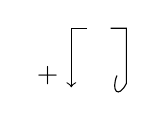
\begin{tikzpicture}[x=1cm,y=1cm]\node at (-.3,0){+};\draw[->](.2,.6)--(0,.6)--(0,-.15);\draw (.5,.6)--(.7,.6)--(.7,-.1) .. controls (.6,-.3) and (.5,-.2) .. (.58,0);\end{tikzpicture}} \unsure{inutile}?}

On peut supposer $S$ noethérien. \deleted{Soit} \inserted{On est ramené à prouver que} $U$ \deleted{\unsure{de} \unsure{plus}} pour un ouvert tel que l'on ait un schéma abélien $A_U$ sur $U$, et $t$ un pt maximal de $S-U=T$, on peut prolonger sur un voisinage $V$ de $t$.

Or \deleted{soit $B$} $V$ un voisinage ouvert de $t$, tel que $A(t)$ provient d'un schéma abélien sur $V$, \deleted{et \deleted{\unsure{soit}} tel que $V$ ne contient pas les $x\in\operatorname{Ass}O_S$ tels que $\unsure{\overline{\{x\}}|\bar x}\unsure{\not\ni|\not\supset}t$, \unsure{Je dis que pour} $\forall s\in V$, \unsure{il y a}}
\inserted{et tel que $B|U\cap V\simeq A_U$}
(isom compatible avec les isom $B\times\operatorname{Spec}O_{S,s}\simeq A(s)$ déjà connus, pour $s\in U\cap\operatorname{Spec}\underline O_{S,t}=:U(s)$). \deleted{Soit} On peut supposer que $x\in\operatorname{Ass}O_S$, $\bar x\unsure{\not\supset|\not\ni}\{t\}\Rightarrow x\notin V$, et que $V\cap\overline T\unsure{\subset|\in}\deleted{\unsure{\overline{\{t\}}}},\deleted{\unsure{t}}$. Soit alors $s\in V\cap\overline T$, donc \inserted{$s\in\overline{\{t\}}$}
\mspage{16}

\scanpage{18}
\margin{\figure{\begin{tikzpicture}[x=1cm,y=1cm]\draw[gray] (0,0)--(.35,1.35)--(.55,1.0);\draw[gray] (.12,.1)--(.34,.8)--(.52,.45);\end{tikzpicture}}}
\deleted{EGA IV $4^{\mathrm o}$ (2èmes épreuves).

P.164\unsure{n|m},note de bas de page, ajouter: ``La Si $f$ est supposé localement de présentation finie ou quasi-projectif, la référence à (18.12.13) peut d'ailleurs se remplacer par une référence à (8.12.8) resp. à (8.12.6).''

Page 165, ligne 9, manque virgule après $X_j$.

Page 166, deux lignes précédant 18.10.8? , les introduire par ``\uline{Remarque} 18.10.17.2.'' , ou (si la place manque), par le seul numéro de référence 18.10.17.2.

Page 187, c'est bien triste d'avoir une démonstration aussi peu parlante de la dernière assertion de (iii), qui est essentiellement triviale et devrait tenir en deux lignes, en \deleted{remarquant} \inserted{utilisant} simplement que si un idéal $\underline J$ est engendré par une suite $\underline O_X$-régulirère $(f_i)$, les $f_i\bmod\underline J^2$ forment une base de $\underline J/\underline J^2$ sur $\underline O_X/\underline J$; cela dit, on trouve évidemment pour le terme médian de (19.1.5.1) une base (localement) se décomposant en deux paquets, dont l'un et l'autre définissent resp. des bases du sous-module et du module quotient. Est-il encore possible de changer le texte en conséquence ?

Page 219, 19.7.5. (i) la référence à (11.3.4) est encore canulée, mettre (6.10.1) !

Page 224, ligne -8, \unsure{ya-t-il|y a-t-il} une référence pour le fait (effectivement vrai) qu'un module est limite inductive \inserted{filtrante} de modules de prés. finie ? Bien sur, on peut toujours s'en tirer en deux crans si on ne veut l'utiliser ($M$ est $\lim$ de ses sous-modules de type fini; un module de type fini est $\lim$ de modules de prés. finie).

Page 225, fin du par. 19, remplacer trois fois F par H (aux lignes -3 et -1 du paragraphe).}

Page 245, référence à $\mathrm{ERR}_{\mathrm{IV}}$ à compléter.
Page 271, ligne 9, manque point-et-virgule après formule.
\mspage{17}

\scanpage{19}
\margin{\figure{\begin{tikzpicture}\node (z) at (0,0){\unsure{Zbl}};\draw (.45,-.28) .. controls (-.9,-.65) and (-.8,.6) .. (.13,.55);\end{tikzpicture}}}
\inserted{d'où $S(t)\unsure{-|\longrightarrow}S(s)$.}
On va définir un \unsure{hom|isom} $\unsure{A(s)}\simeq B\times_{\deleted{\unsure{V}}S}\unsure{S(s)}$, tel que par \unsure{chgt de base} $S(t)\longrightarrow S(s)$, on retrouve l'isom $A(t)\simeq B\times_S S(t)$ donné. \deleted{Un tel \unsure{isom}}

\uline{Lemme} $S$ schéma \unsure{noethérien|noeth.}, \inserted{\deleted{[excellent]}} $t\in S$, $B$ schéma abélien sur $S$. Alors $\exists$ voisinage ouvert $V$ de $t$, \deleted{\unsure{avec} \unsure{les} \unsure{comp.} \unsure{de} \inserted{\deleted{\unsure{irréduc.}}}} tel que pour \deleted{$\unsure{\Rightarrow}\ \forall s\in V$,} tout voisinage ouvert $\unsure{W'|V'}$ de $t$, $V'\subset V$, tout schéma abélien $B'$ sur $V'$, et tout isom $\varphi_0:B'\times_S\operatorname{Spec}O_{S,t}\simeq B\times_S\operatorname{Spec}\underline O_{S,t}$, $\varphi_0$ se prolonge (de façon unique en un isom $\varphi:B'\simeq B|V'$.

L'unicité sera garantie dès que \unsure{toute composante} \unsure{ponctuelle|point associé} de $V$ rencontre $t$, i.e. que $V$ est contenu dans \unsure{la réunion|le complément} des comp. irréduc. de $S$ ne contenant pas $t$.

\deleted{Soit $S'\longrightarrow S$}
On peut supposer $S$ affine. \inserted{Supposons d'abord $S$ excellent.} Soit $S'\longrightarrow S$ fini, tel que $S'\times_S S(s)\longrightarrow S(s)$ soit birationnel, et $S'$ réduit et géom. unibr.

Alors
\mspage{18}

\scanpage{20}
\begin{flushright}14 MARS 1967\end{flushright}
\figure{\begin{tikzpicture}[x=1cm,y=1cm]
\node[draw,circle,inner sep=2pt] at (1.5,1.0){\mspage{1}};
\node[draw,ellipse,minimum width=2.1cm,minimum height=1.8cm] at (0,-.3){17.1.6};
\node[draw,ellipse,rotate=12,minimum width=2.5cm,minimum height=1.7cm] at (-.05,-1.8){\rotatebox{-12}{19.1.8}};
\node[draw,ellipse,rotate=10,minimum width=2.6cm,minimum height=1.7cm] at (-.2,-3.25){\rotatebox{-10}{19.4.11}};
\node at (0,-4.8){(\unsure{18.32.1|18.12.1})};
\end{tikzpicture}}
\begin{center}
\textbf{PUBLICATIONS}\\
\textbf{MATHÉMATIQUES}\\[1em]
\textbf{N\textsuperscript{o} 32}
\end{center}
\figure{\begin{tikzpicture}[x=1cm,y=1cm]
\draw[gray] (0,0) .. controls (.35,.13) and (.35,.5) .. (.32,.75)--(.8,.55);
\draw[gray] (1.5,1)--(1.5,2);\draw[gray] (1.48,1.55)--(1.8,1.55);\draw[gray] (1.8,1)--(1.8,1.8);
\draw[gray,line width=2pt,opacity=.4] (2.25,-.2)--(2.65,2);
\draw[gray] (3.25,0) .. controls (3.5,.7) and (3.6,1.65) .. (3.4,2);
\end{tikzpicture}}
\begin{flushright}\textit{Bon à tirer}\\\textit{(Date et Signature, S.V.P.)}\end{flushright}
\mspage{19}

\scanpage{21}
\diagram{\begin{tikzcd}[ampersand replacement=\&,column sep=small,row sep=small]A\arrow[dr,dash]\&\&B\arrow[dl,dash]\\\&S\&\end{tikzcd}}
\margin{schémas abéliens sur $S$}
\[
u_p:T_p(A)\mathbin{-}T_p(B)
\]
Question: quand \unsure{ceci} provient-il d'un hom $u:A\mathbin{-}B$.
\deleted{(i) À cause de l'unicité, \unsure{la desc est fid. plate universelle}}
\deleted{(ii) l'ens \inserted{$T$} des pts $s\in S$ tels que $u_{ps}:T_p(A_s)\mathbin{-}T_p(B_s)$ provienne de $u_s:A_s\longrightarrow B_s$ (condition géom. par (i)) est \uline{fermé}.
\deleted{Si $t\in T$ est tel que car. $k(t)=$}
(iii) Si $t\in T$ est tel que car $k(t)=p$, alors $\exists$ voisinage ouvert $U$ de $t$ tel que $u_p|U$ soit algébrique, en particulier \unsure{$t$ est un pt intérieur de $T$}.}

\figure{\begin{tikzpicture}[x=1cm,y=1cm]
\draw (0,0)--(.15,3.3);\draw (0,0) .. controls (1.4,.1) and (2.8,.04) .. (3.65,.48) .. controls (4.5,1.0) and (5.5,1.2) .. (5.8,2.05)--(6,4.0);
\draw[line width=.8pt] (0,0) .. controls (.6,1.9) and (1.4,3.2) .. (2.6,4.0);
\draw[line width=.8pt] (.8,.07) .. controls (1.25,1.9) and (2.2,3.3) .. (3.75,4.0);
\draw[line width=.8pt] (1.6,.12) .. controls (2,2.0) and (3.3,3.4) .. (4.9,4.0);
\draw[line width=.8pt] (2.25,.18) .. controls (2.8,2.1) and (4,3.5) .. (5.95,4.1);
\draw[line width=.8pt] (3.15,.28) .. controls (3.9,2.1) and (4.8,2.9) .. (6,3.4);
\draw (1.55,2.9) .. controls (1.4,1.7) and (2.1,1.6) .. (2.0,1.25);\node at (1.45,1.6){$S$};\node at (2.3,1.5){\deleted{$\unsure{s_0}$}};
\draw (3.25,.5)--(3.6,1.8)--(3.4,2.2)--(4.15,1.85);\node at (4.1,2.05){$\unsure{S''_0|S'_0}$};\node at (5.1,2.15){$S'$};\draw[->,thick](4.85,2.12)--(4.35,2.02);
\draw (3.6,3.65) .. controls (4,3.75) and (3.8,2.75) .. (4.2,2.5);\draw (5.4,3.5) .. controls (5.7,3.55) and (5.4,2.45) .. (5.8,2.35);
\node at (4.65,3.0){$\unsure{A_{s'}|A_{S'}}$};\node at (5.8,3.0){$\unsure{B_{s'}|B_{S'}}$};\draw[->](5.0,3.05)--(5.45,3.05);
\fill (.3,-.08) circle (1.5pt);\draw (.3,-.08) ellipse (.25 and .3);\draw[thick](-.3,-.08)--(.3,-.08);
\end{tikzpicture}}

a) Il y a \inserted{(si $S$ noeth)} un plus grand sous-schéma $\unsure{\overline S|T}$ de $S$ sur lequel $u_p$ est algébrique; $T$ est fermé, sa \unsure{formati-} commute à tout changt de base (nouvelles bases pas \unsure{néc.} noethériennes).

b) Si $t\in T$ est tel que car $k(t)=p$, alors $T$ contient un voisinage ouvert induit de $t$. \deleted{Donc si $S_p=V(p1_S)$, alors $T$ est un voisinage (\unsure{ouvert-et-fermé}) de $T\cap S_p$}

\deleted{\uline{Cor.} Supposons que pour tout $s\in\operatorname{Ass}O_S$,}
\deleted{\uline{Corollaire} Supposons que pour tout $s\in$}

\uline{Cor.} Soit $Z$ l'ens \deleted{des éléments de $\operatorname{Max}S$ \unsure{et de} (pts maximaux de $S$) et de l'ens des} \inserted{des pts de $S$ qui sont} maximaux, ou qui sont associés \deleted{\unsure{et}} à $O_S$ \uline{et} de car. $\ne p$. Supposons que $z\in Z\Longrightarrow\exists s\in\overline{\{z\}}$ tel que $k(s)$ de car. $p$ et $s\in T$ \inserted{(i.e. $\overline{\{z\}}\cap S_p\cap T\ne\varnothing$)}. Alors $u_p$ est algébrique.
\mspage{20}

\scanpage{22}
\deleted{$A\mathbin{-}A'$}
\deleted{\deleted{$\unsure{A}$}\quad $A'\quad\deleted{T_p(\unsure{A'})}\quad A''\qquad T_p(\unsure{A''_i|A'_i})\simeq T_p(\unsure{A'_i|A''_i})$}
\deleted{\diagram{\begin{tikzcd}[ampersand replacement=\&,column sep=small,row sep=small]S\arrow[r,dash]\&S'\arrow[r,equal]\&S''\\y\arrow[r,dash]\&y'\&y''=y'\amalg y'\end{tikzcd}}}
\deleted{$S-T=T\times_{\unsure{y}}T=T\amalg T$}
\deleted{$T\amalg\uline{T}\amalg\uline{T}$}

\mspage{-0.9-}
then $Y$ is noetherian, or even locally noetherian in all cases (this is an analog of Hilbert's 14th problem). I only know one fact in this direction: if $S=\operatorname{Spec}(k)$, $k$ a field, $X$ is a normal algebraic scheme over $k$, and $(Y,\phi)$ is a \uline{geometric} quotient, then $Y$ is an algebraic scheme over $k$. Since we have no use for this, I omit the proof.
\figure{\begin{tikzpicture}\draw[gray](0,0)--(.04,1.9);\draw[gray](.1,0)--(.13,1.9);\end{tikzpicture}}

(3) Suppose $(Y,\phi)$ is a universal categorical quotient. Applying this assumption to the base extensions given by the inclusion of open subsets $U$ in $Y$, one deduces condition (iv) of definition 0.6. More-over, applying it to the inclusion of a single point $y$ in $Y$, and noting that the categorical quotient of an empty scheme by any group is an empty scheme, one deduces that $\phi$ is surjective. Therefore, for $(Y,\phi)$ to be a universal geometric quotient, it is necessary and sufficient that (1) $\phi$ is universally submersive, and (2) the image of $\unsure{\overline{\underline{\psi}}|\overline{\underline{\Psi}}}$ is $X\times_Y X$.

(4) Suppose that the projection from $G$ to $S$ is universally open. This occurs if the projection is flat and of \inserted{loc} finite \figure{\begin{tikzpicture}[baseline=(t.base)]\node[draw,ellipse,inner sep=1pt](t){type};\end{tikzpicture}}, hence for example if $S=\operatorname{Spec}(k)$, $k$ a field, and $G$ is an algebraic group (cf. SGA 4). More generally, this occurs if $S$ is an irreducible normal noetherian pre-scheme, the projection from $G$ to $S$ is \inserted{loc} of finite type, all components of $G$ dominate $S$, and all geometric fibres of $G$ over $S$ have the same dimension: this is Chevalley's
\margin{\unsure{présentation}}
\mspage{21}

\scanpage{23}
\uline{Lemme} 1 Soit $f:S'\longrightarrow S$ un épimorphisme propre de schémas [\inserted{loc} noethériens], et \deleted{$\unsure{Z}$} $X$ un schéma \inserted{formellement} non ramifié sur $S$. Alors la suite
\margin{\figure{\begin{tikzpicture}\node[align=left,text width=2cm,inner sep=2pt](m){[\ ]\\inutile si\\$X$ \uline{loc}\\de t.f.?};\draw (m.north west) .. controls +(2.5,0) and +(.8,.8) .. (m.south east);\draw (m.south east) .. controls +(-.7,-.2) .. (m.south west);\draw (m.east) .. controls +(0,-.4) and +(1,0) .. (m.south west);\end{tikzpicture}}}
\diagram{\begin{tikzcd}[ampersand replacement=\&,column sep=large]\operatorname{Hom}_S(S,X)\arrow[r]\&\operatorname{Hom}_S(S',X)\arrow[r,shift left=.5ex]\arrow[r,dash,shift right=.5ex]\&\operatorname{Hom}_S(S'',X)\end{tikzcd}}
est exacte, où $S''=S'\times_S S'$.

\unsure{NB} le fait que $f$ est un épimorphisme s'exprime par la condition que l'hom
\[
\underline O_S\longrightarrow f_*(O_{S'})
\]
est \uline{injectif}.

Soit $g':S'\longrightarrow X$ tel que $g'\operatorname{pr}_1=g'\operatorname{pr}_2$, à montrer que $g'$ se factorise par $S$. Tout d'abord il se factorise par $S$ en \unsure{prenant} une application continue, soit $g_0$, et
\[
f^{-1}(g_0^{-1}(\underline O_X))\simeq g'^{-1}(O_X)\longrightarrow O_{S'}
\]
adjoint un hom
\[
g_0^{-1}(O_X)\longrightarrow f_*(O_{S'});
\]
\diagram{\begin{tikzcd}[ampersand replacement=\&,column sep=small,row sep=small]\&\&X\arrow[d]\\S''\arrow[r,shift left=.5ex,"p_1"]\arrow[r,shift right=.5ex,"p_2"']\arrow[rr,bend right=30,"h"']\&S'\arrow[ur,"g'"]\arrow[r,"f"']\&S\arrow[u,dashed,bend right=20,"g_0"']\end{tikzcd}}
l'hyp. $g'\operatorname{pr}_1=g'\operatorname{pr}_2$ s'exprime par le fait que $g_0^{-1}(\underline O_X)$ s'envoie dans
\[
\mathcal A=\operatorname{Ker}(f_*(O_{S'})\rightrightarrows\deleted{\unsure{f_*}}h_*(\underline O_{S''}))
\]
donc $g'$ se factorise par
\[
S'\longrightarrow\operatorname{Spec}(\mathcal A)=S'_1\longrightarrow X.
\]
Or EGA III 3 implique évidemment que $S'_1\longrightarrow S'$ est \inserted{fini,} \uline{radiciel}, c'est d'ailleurs un épimorphisme car $\underline O_S\hookrightarrow\deleted{\unsure{f_*\underline O_S}}\mathcal A\hookrightarrow f_*(O_{S'})$, $f$ étant un épimorphisme. On est donc ramené à prouver le
\margin{\uline{lemme}}

\uline{Corollaire} 1 Soit $f:S'\mathbin{-}S$ un épimorphisme de schémas \deleted{\unsure{noethériens}}, $f$ \deleted{fini} \inserted{entier} radiciel, et $X$ \deleted{non ramifié} \inserted{\deleted{loc de t.f.}\unsure{formelt}} sur $S$; \deleted{\unsure{Alors $f$ fini}} \inserted{(on \unsure{suppose} $f$ fini et $S$ loc. noeth, ou $X\mathbin{-}S$ loc. de t.f.)} Alors
\[
\operatorname{Hom}_S(S,X)\mathbin{-}\operatorname{Hom}_S(S',X)\quad\text{est \uline{bijectif}}.
\]
\mspage{22}

\scanpage{24}
\begin{center}-\mspage{0.16 bis}-\end{center}
\[
\operatorname{tr.d.}\ \unsure{\kappa|\mathcal K}(y)/k+\sigma(y)=\dim G.
\]
Now if the action were not closed, at least over some $k$ there would be two points $x_1,x_2\in X_k$ such that $O(x_2)\subset\overline{O(x_1)}-O(x_1)$. Let $y_i$ be the generic point of $O(x_i)$. Since $x_2$ is a regular point of the action, one finds that $\sigma(x_1)=\sigma(x_2)$, hence
\[
\operatorname{tr.d.}\ \unsure{\kappa|\mathcal K}(y_1)/k=\operatorname{tr.d.}\ \unsure{\kappa|\mathcal K}(y_2)/k<\infty.
\]
But $y_2$ is a specialization of $y_1$, hence this is absurd.

Concerning restrictive conditions on the action of $G$, a notion intermediate between the closedness of one orbit and the properness of the whole action is sometimes convenient:

\uline{lemma} \uline{0.3}: Let $S=\operatorname{Spec}(k)$, $k$ an algebraically closed field, and assume $X$ and $G$ are algebraic pre-schemes over $k$. Let $\sigma$ be an action of $G$ on $X$, and let $x\in X_k$. Then $\psi_x$ is proper if and only if $O(x)$ is closed in $X$ and $S(x)$ is proper over $k$.

\uline{Proof}: If $\psi_x$ is proper, then its image $O(x)$ must be closed, and its fibre over $x$ - which is $S(x)$ - must be proper over $k$.

On the other hand, assume that $O(x)$ is closed and $S(x)$ is proper over $k$. To prove that $\psi_x$ is proper, we may as well replace $G$
\mspage{23}

\scanpage{25}
Pour le voir, \deleted{\unsure{on remarque aussitôt}} \inserted{comme c'est évidemment injectif,} on est ramené à prouver que c'est surjectif. Soit $g':S'\mathbin{-}X$ prouvons que ça se factorise par $S$.
\deleted{Or $g'$ \unsure{définit une section de} $X'=X\times_S S'$ sur $S'$, \unsure{donc une partie ouverte} de $X'$, \inserted{car $X'/S'$ est \unsure{formelt net},} comme $X'\longrightarrow X$ est un homéomorphisme, on conclut que $g'(S')$ est une partie \unsure{à la fois ouverte et fermée} de \deleted{\unsure{X}} $X$, et en \unsure{remplaçant} $X$ par \unsure{le} \illegible{2}}
\inserted{Comme $S'\longrightarrow S$ est un homéo-morphisme, on est ramené trivialement au cas où $S$, donc $S'$, local, de pt fermé $s$, \unsure{resp.} $s'$, et à prouver que (si $x=g'(s')$) $\underline O_{X,x}\mathbin{-}O_{S',s'}$ se factorise par $O_{S,s}$.}
\diagram{\begin{tikzcd}[ampersand replacement=\&,column sep=small,row sep=small]\&\underline O_{X,x}\arrow[dl]\\O_{S',s'}\&O_{S,s}\arrow[u,hook]\arrow[l,hook]\end{tikzcd}}
\deleted{Remplaçant $X$ par un voisinage affine de $x$, on peut supposer $X$ affine, donc \unsure{supposer} $X\longrightarrow S$ \unsure{affine}, \unsure{il suffit}, et alors \unsure{supposer} $X$ \unsure{égal à} $g'(S')$ et $g'$ est \unsure{surjectif}, \unsure{car} \illegible{2}. Mais alors \unsure{local} \illegible{2} $S$.}
\unsure{fermé}. Remplaçant $X$ par l'image \inserted{\uline{schématique}} de $g'$, on peut supposer
\deleted{\unsure{Mais} $\unsure{O_S}\hookrightarrow A\hookrightarrow f_*O_{S'}$, \unsure{et on a} \unsure{$\unsure{I}A$}, et comme $\underline O_S\longrightarrow A$ est injectif, \unsure{on conclut que} $g'$ \unsure{est fidèle}, \unsure{et donc}}
\inserted{que $X$} est \deleted{\unsure{donc}} local, de pt fermé $x$, et $\underline O_{X,x}\hookrightarrow O_{S',s'}$. Alors $\underline O_{X,x}$ est donc entier sur $O_{S,s}$, et $=$ \unsure{par un} $O_{S,s}$ si $f$ fini et $S$ loc noeth.

\uline{Corollaire} 2 Soit $f:\inserted{S'\longrightarrow S}$ un épimorphisme propre de schémas noethériens. Alors $f$ est un morphisme de descente pour la catégorie des schémas abéliens relatifs.
\figure{\begin{tikzpicture}\draw[line width=1pt](0,0)--(-.05,1.5);\end{tikzpicture}}

Si $A$ et $B$ sont deux schémas abéliens sur $S$, on sait en effet que $H=\underline{\operatorname{Hom}}_S(A,B)$ est représentable, et est net sur $S$, donc il suffit d'appliquer le lemme 1.

\uline{Corollaire} 3 Soit $p$ un nb premier, et soit $f:S'\mathbin{-}S$ comme dans le cor. précédent. Alors $f$ est un morphisme de descente pour la catégorie des \deleted{\unsure{gr}} schémas en groupes $p$-divisibles.

L'argument \deleted{\unsure{préc.}} du lemme 1 nous ramène à prouver l'analogue du corollaire 1, quand $X=\underline{\operatorname{Hom}}_S(A,B)$, $A,B$ deux groupes $p$-divisibles. Il faut prouver que $X$ est formellement net.
\mspage{24}

\scanpage{26}
\mspage{iv}
the Italian school: to give an algebraic proof of the completeness of the characteristic linear system of suitable complete continuous sys-tems on a surface in characteristic 0 (cf. [13], [18], [33] and [36]).

It is my pleasure to acknowledge at this point the great encourage-ment and stimulation which I have received from Oscar Zariski, John Tate, and Alexander Grothendieck. In addition, I want to give credit to the many sources from which I have taken a great deal:

Ch. 1 and 2 owe a great deal to D. Hilbert [14],

\S1.2. was developed independently by C. Chevalley, N. Iwahori, and M. Nagata,

\S2.2. is largely a theory of J. Tits,

Ch. 3 was worked out by J. Tate and myself,

\S4.3. includes an example of M. Nagata

\S4.5. is a theorem of B. Kostant,

In Ch. 5 and 7, the whole approach to moduli via functors is due to A. Grothendieck,

\S5.3. and \S5.4. follow suggestions of A. Grothendieck,

Ch. 6 is almost entirely the work of A. Grothendieck.

\begin{flushright}Harvard University\\Oct. 27, 1963\end{flushright}
\mspage{25}

\scanpage{27}
Soit $f$ comme dans Cor. 2, \inserted{mais on suppose $f$ un épi. effectif.} On veut prouver que $f$ est un morphisme de descente \uline{effective}. Soit donc $A'$ schéma abélien sur $S'$, avec donnée de descente relativement à $S'\mathbin{-}S$; prouver que cette donnée est effective.

a) Réduction au cas $S$ local \inserted{$=\operatorname{Spec}R$}: \uline{triviale}, par passage à la limite.
\deleted{\unsure{On y procède par récurrence sur} \illegible{3}, \unsure{sachant que le cas} \illegible{1} \unsure{est effectif dans le cas formel des schémas affines}.}

b) Réduction au cas $S$ local complet: \unsure{coup usuel} Alg. des.

Grâce au critère de descente plate des schémas abéliens de Raynaud. Mais il faut savoir que $S'_2\mathbin{-}S_2$ est \inserted{morphisme} de descente pour la catégorie des schémas abéliens relatifs, et on ne peut directement appliquer le \deleted{lemme 1, car} cor. 2, car $S_2$ n'est plus loc. noeth! Mais on s'en tire en remarquant qu'il est vrai \deleted{\unsure{que l'on}} ici que (avec les notations de la dém. du lemme 1)
\diagram{\begin{tikzcd}[ampersand replacement=\&,column sep=small,row sep=small]
S\arrow[r,dash]\arrow[d,dash]\&S'\arrow[r,equal]\arrow[d,dash]\&S''\arrow[r,equal]\arrow[r,dash]\&S'''\&\text{1-descente}\\
S_1\arrow[r,dash]\arrow[d,equal]\&S'_1\arrow[r,equal]\arrow[d,equal]\&S''_1\arrow[r,equal]\arrow[r,dash]\arrow[d,equal]\&S'''_1\arrow[d,equal]\&\text{1-descente}\\
S_2\arrow[r,dash,"f_2"']\arrow[d,equal]\arrow[d,dash]\&S'_2\arrow[r,equal]\arrow[d,equal]\arrow[d,dash]\&S''_2\arrow[r,equal]\arrow[r,dash]\arrow[d,equal]\arrow[d,dash]\&S'''_2\arrow[d,equal]\arrow[d,dash]\&\text{1-descente}\\
S_3\arrow[r,dash]\&S'_3\arrow[r,equal]\&S''_3\arrow[r,equal]\arrow[r,dash]\&S'''_3\&\text{0-descente}
\end{tikzcd}}
\deleted{$A$ est radiciel sur \unsure{\text{$h_2$}} $f_2$}
\[
\operatorname{Ker}(f_{2*}O_{S'_2}\rightrightarrows h_{2*}(O_{S''_2}))
\]
est radiciel sur $\underline O_{S_2}$, car tout provient par chgt de base plat de la situation
\[
O_S\longrightarrow\operatorname{Ker}(f_*(O_{S'})\rightrightarrows h_*(O_{S''})).
\]
\margin{\figure{\begin{tikzpicture}\node[align=left,text width=3cm,inner sep=2pt](m){donner remarque après lemme 1; donne aussi le \unsure{cas de} 0-descente};\draw[gray] (m.north west) .. controls +(2,0) .. (m.north east);\draw (m.north east) -- ([xshift=8pt]m.east) .. controls +(0,-.8) and +(1,0) .. (m.south west);\end{tikzpicture}}}

\deleted{c) \deleted{\unsure{Cas à 2 étages}} Cas \deleted{$\unsure{S}$ dim $S=0$.} \inserted{$S$ réduit dim $S=0$ (et \unsure{le corps résiduel alg. clos})} On se ramène au cas où $S'$ est fini sur $S$ (quitte à prendre un sous-schéma fini \deleted{\unsure{de $S'$}} assez gros de $S'$), puis par \uline{factorisation}, se ramener au cas où $\operatorname{long}_A A'/A=1$. Alors le critère de descente par plate \unsure{est vérifié}: \unsure{trouver des} ouverts affines recouvrant $A'$, stables par \deleted{\unsure{des}} données de descente. Or pour ça, on est ramené au cas où $A$ est le spectre d'un corps, où c'est trivial.
\margin{\deleted{expliciter du point de vue \unsure{``carré de descente''}}}

d) Construction d'un schéma formel \inserted{abélien} sur $\operatorname{Spf}R$, qui descend le schéma formel défini par $A'$ (complété suivant la fibre de $A'_s$\unsure{\ldots}). \deleted{\unsure{Immédiat}} \inserted{Facile} \unsure{preuve}).}
\mspage{26}

\scanpage{28}
\mspage{-0.4-}
\uline{Definition} \uline{0.4}: Let $f:T\longrightarrow X$ be a $T$-valued point of $X$. Then $\sigma\circ(1_G\times f)$ is a morphism from $G\times_S T$ to $X$. Define the morphism
\[
\psi_f^G:G\times_S T\longrightarrow X\times_S T
\]
as $(\sigma\circ(1_G\times f),p_2)$. If no confusion arises, $\psi_f^G$ will be shortened to $\psi_f$. If $f=1_X$, $\psi_f$ will be denoted $\unsure{\overline{\underline{\psi}}|\overline{\underline{\Psi}}}$. $\unsure{\overline{\underline{\psi}}|\overline{\underline{\Psi}}}$ is simply:
\[
(\sigma,p_2):G\times_S X\longrightarrow X\times_S X.
\]
The image of $\psi_f$ will be denoted $O(f)$ and called the \uline{orbit} of $f$. Now $X\times_S T$, as a scheme over $T$, has a canonical section, namely $(f,I_T)$. Via this, we set up a fibre product defining $S(f)$:
\diagram{\begin{tikzcd}[ampersand replacement=\&]S(f)\arrow[r]\arrow[d]\&T\arrow[d,"{(f,I_T)}"]\\G\times_S T\arrow[r,"\psi_f"]\&X\times_S T.\end{tikzcd}}
Now $G\times_S T$ is, of course, a group pre-scheme over $T$, and it is not hard to show that $S(f)$ is a subgroup pre-scheme over $T$. If is called the \uline{stabilizer} of $f$.

In case $T=\operatorname{Spec}(k)$, and $f$ is a closed immersion of a point $x\in X$ into $X$, we shall also write $O(x)$ for $O(f)$, and $S(x)$ for $S(f)$. In case $T=\operatorname{Spec}(\Omega)$ and $\Omega$ is an algebraically closed field, then $f$ is a geometric point of $X$, and it will usually be denoted by a letter $x,y$, etc. Then note that $O(x)$ is a subset of
\mspage{27}

\scanpage{29}
d) \uline{Construction d'un schéma abélien formel}.

Notons d'abord que si $S_0=\operatorname{Spec}k$ ($k$ corps résiduel) alors $S'_0/S_0$ - \unsure{une galér|une galère}, donc $S'_0\mathbin{-}S_0$ est un morphisme de descente effective universelle, et on trouve un $A_0$ sur $S_0$ qui descend $A'_0$.
\diagram{\begin{tikzcd}[ampersand replacement=\&,column sep=small,row sep=small]
\&\&\widehat A'\&\widehat A''\&\widehat A'''\\
M\arrow[dd]\&S_0\arrow[l]\&S'_0\arrow[l]\&S''_0\arrow[l,shift left=.5ex]\arrow[l,shift right=.5ex]\&\\
\&\&\&\&\\
\unsure{T|\overline T}\&\widehat S\arrow[l]\&\widehat S'\arrow[l,dash]\&\widehat S''\arrow[l,shift left=.5ex]\arrow[l,shift right=.5ex]\&\widehat S'''\arrow[l,shift left=.8ex]\arrow[l]\arrow[l,shift right=.8ex]\\
\&S_0\arrow[r,dash]\&S'_0\arrow[r,equal]\&S''_0\arrow[r,equal]\arrow[r,dash]\&S'''_0
\end{tikzcd}}

Commençons par prendre les complétés formels de $S',S'',S''',A',A'',A'''$ \deleted{\unsure{sur}} relativement aux fibres de $s$, on trouve \deleted{\unsure{un}} schéma abélien formel $\widehat A'$ sur $\widehat S'$, avec donnée de descente pour $\widehat S'\mathbin{-}\widehat S$. On va commencer à descendre dans la catégorie des schémas abéliens formels.

On introduit $\overline T=\operatorname{Spf}W(k)$ ($W$ anneau de Witt) et $M=$ schéma formel des modules de $A_0$ ($M$ considéré comme schéma formel). Un lemme facile qui est \unsure{pratiquement} trivial si $S'$ fini sur $S$ [donc $\widehat S',\widehat S''$, \unsure{etc.} sont pro-artiniens] dit que la donnée d'une extension \inserted{formelle} $\widehat A'$ de $A'_0=A_{0S'_0}$ [resp $\widehat A''$ de $A''_0$] équivaut à la donnée d'un $\overline T$-morphisme $\varphi':\widehat S'\longrightarrow M$ [resp. $\varphi'':\widehat S''\mathbin{-}M$] \deleted{\unsure{resp.} $\widehat S'''\mathbin{-}M$]}.
La donnée de descente \inserted{sur $A'$} prolongeant celle que l'on avait sur $A'_0$ équivaut à la condition $\varphi'\widehat p_1=\varphi'\widehat p_2$. On en \unsure{conclut|déduit} aussitôt (\unsure{évidemment}, trivial encore si $S'$ fini sur $S$, et provient du Th. de comparaison formel-algébrique en général) que la suite
\diagram{\begin{tikzcd}[ampersand replacement=\&]\widehat S\&\widehat S'\arrow[l]\&\widehat S''\arrow[l,shift left=.5ex]\arrow[l,shift right=.5ex]\&\deleted{\unsure{\leftleftarrows}}\end{tikzcd}}
de schémas formels est exacte, donc on trouve $\varphi:\widehat S\mathbin{-}M$ tel que $\varphi\widehat f=\varphi'$. Cela signifie qu'on a pu descendre
\mspage{28}

\scanpage{30}
\margin{\illegible{1} \unsure{MARAIS}}
\deleted{
\begin{flushright}Paris, le 24 Février 1968\end{flushright}

Cher Grothendieck,

J'espère que ta grippe est terminée, et que tu es maintenant complètement rétabli.

Je t'adresse ici l'Exp. IV, que tu devrais recevoir lundi si la poste marche bien. Alors que je terminais l'appendice (R-R en Géométrie Analytique), je me suis aperçu que tu avais déjà traité la question dans Exp. 0 : il faudra peut-être le vider.

Je joins ma demande de renouvellement pour le CNRS, en te demandant si tu pourrais me l'apostiller. Les années précédentes, Cartan s'en chargeait, mais il estime maintenant que tu es mieux placé que lui pour le faire.

Dès que je pourrai, en principe dans une semaine, je t'en-verrai mes prénotes sur Künneth.

\begin{flushright}Bien à toi,\end{flushright}
}
\begin{flushright}L Illusie\end{flushright}
\margin{\unsure{RAIS}}
\mspage{29}

\scanpage{31}
$\widehat A'$ en un schéma formel abélien $\widehat A$.

Le th. de comparaison alg. formel nous ramène à prouver que $A$ est algébrique.

On est ainsi ramené à prouver le

\uline{Th.} Soit $R$ anneau loc noeth complet, $S=\operatorname{Spec}R$, $\widehat A$ un schéma \inserted{abélien formel} abélien sur $\widehat S=\operatorname{Spf}\unsure{B|R}$. Conditions équivalentes

(i) $\widehat A$ \unsure{algébrique}, i.e. $\exists$ schéma abélien $A$ sur $S$, tel que $\widehat A$ soit isom. à son complété formel le long de $A_s$.

(ii) $\exists$ morphisme propre \uline{surjectif} \deleted{\unsure{surjectif}} $f:S'\longrightarrow S$, \deleted{\unsure{et}} tel que l'image inverse $\widehat A'$ de $\widehat A$ sur $\widehat S'$ soit algébrique.

(iii) Pour toute \deleted{algèbre finie $B$ sur $A$} quotient \deleted{fini} \inserted{intègre} $B$ de $A$, de dim $1$, si $B'$ est le normalisé de $B$, et \deleted{$\unsure{\widehat B}$} $\widehat T'=\unsure{\operatorname{Specf}|\operatorname{Spf}}B'$, --- $\widehat A_{\widehat T'}$ est algébrique.

\margin{\figure{\begin{tikzpicture}\node[align=left,text width=4cm,inner sep=3pt](m){\uline{NB} La démonstration \unsure{montre} qu'on peut se borner \uline{aux} $x\in S$, $\dim\{\unsure{\bar x|x}\}=1$, qui ne sont pas contenus dans les $\bigcup_i T_i$, où les $T_i$ sont \deleted{\unsure{des}} \unsure{fermés} dans $S$ de \unsure{toute} famille \uline{dénombrable}.};\draw (m.north west) .. controls +(2,0) and +(1,.5) .. (m.east) .. controls +(-.8,-1) and +(2,0) .. (m.south west);\end{tikzpicture}}}

\deleted{N.B. On peut \unsure{démontrer} le th. si $\dim R=1$, et en utilisant \unsure{l'algébricité} de l'espace des \unsure{faisceaux}.}

\uline{Dém.} $(i)\Longrightarrow(ii)$ est trivial.

$(ii)\Longrightarrow(iii)$ Car introduisant $T'=S'\times_S T$, on voit que $\widehat T'\mathbin{-}\widehat T$ ``rend $\widehat A_{\widehat T}$ algébrique''. Or on peut trouver, comme $T$ est un trait complet, un trait $T_1$ \deleted{et plat} \inserted{(fini sur $T$)}, et un $T$-morphisme $T_1\mathbin{-}T'$. Donc $\widehat A_{\widehat T_1}$ est algébrique, donc définit un schéma abélien $A_{T_1}$ sur $T_1$. Ce dernier est muni d'une donnée de descente rel à $T_1\mathbin{-}T$ [grâce au th. de comparaison], il suffit \deleted{\unsure{encore}} de voir que la donnée est effective, ce qui est évident, car $T_1\mathbin{-}T$ est \inserted{fid} plat fini, et $A_1$ est projectif.

\margin{\figure{\begin{tikzpicture}\node[align=left,text width=4cm,inner sep=3pt](m){\deleted{Pour \unsure{utiliser} \unsure{le th.}, la \unsure{N.Q.|N.O.} \unsure{sur} $\unsure{x}$ \unsure{implique} \unsure{de} \unsure{lui|limite} \unsure{imposer} une famille \unsure{indénombrable} \unsure{à éviter}.}};\draw (m.north west) -- ([xshift=5pt]m.north east) .. controls +(0,-1) .. (m.south east) -- (m.south west) -- (m.north west);\end{tikzpicture}}}

\mspage{30}

\scanpage{32}
\mspage{-0.2-}

projective $n$-space \uline{over} $\underline{\mathbb Z}$, unless, in a particular chapter, all considerations are over a ground field $k$, in which case they will denote affine $n$-space and projective $n$-space over $k$. $\operatorname{PGL}(n)$ will be the projective group acting on $\mathbb P_n$, $\operatorname{GL}(n)$ the general linear group acting on $\mathbb A^n$, and $\mathbb G_m=\operatorname{GL}(1)$. The same conventions on the base scheme hold for these group schemes.

(6) $1_X$ is the identity morphism from $X$ to $X$. $p_1$ and $p_2$ are the projections from $X\times_S Y$ to $X$ and $Y$; $p_{12}$, etc. are the projections from $X\times_S Y\times_S Z$ to $X\times_S Y$, etc. If $f:X_1\longrightarrow X_2$ and $g:Y_1\longrightarrow Y_2$ are $S$-morphisms, then $f\times g:X_1\times_S Y_1\longrightarrow X_2\times_S Y_2$ is the product. If $f:X\longrightarrow Y_1$ and $g:X\longrightarrow Y_2$ are $S$-morphisms, then $(f,g):X\longrightarrow Y_1\times_S Y_2$ is the induced $X$-morphism.

(7) If $X$ is a pre-scheme, and $x\in X$, then $\unsure{\kappa|\mathcal K}(x)$ will denote the residue field of $\underline o_{x,X}$. If $X$ is a scheme over a field $k$, $X_k$ will denote the set of points $x\in X$ such that $k\xrightarrow{\sim}\unsure{\kappa|\mathcal K}(x)$.

\margin{\figure{\begin{tikzpicture}[scale=.5]\draw[gray!40] (0,0)--(.5,-.02) .. controls (1,-.05) and (1,.35) .. (.52,.4);\draw[gray!40] (.3,0)--(.31,.36);\end{tikzpicture}}}

\fbox{\S1.} \uline{Definition} \uline{0.1}: A group pre-scheme $G/S$ is a morphism $\pi:G\longrightarrow S$ of pre-schemes, plus $S$-morphisms $\mu:G\times_S G\longrightarrow G$, $\beta:G\longrightarrow G$, $e:S\longrightarrow G$ satisfying the usual identities:

(a) \uline{Associativity}:
\diagram{\begin{tikzcd}[ampersand replacement=\&]
G\times_S G\times_S G \arrow[r,"1_G\times\mu"] \arrow[d,"\mu\times1_G"'] \& G\times_S G \arrow[d,"\mu"] \\
G\times_S G \arrow[r,"\mu"] \& G
\end{tikzcd}} commutes.

\mspage{31}

\scanpage{33}
\deleted{$(iii)\Longrightarrow(i)$ (cas $R$ réduit)}

\[
(iii)\Longrightarrow\quad (ii')\left\{\begin{gathered}\exists\text{ morphisme }\deleted{\text{un}}\text{ fini surjectif net }S'\longrightarrow S\text{ tel que}\\ \widehat A_{\widehat S'}\text{ soit algébrique.}\end{gathered}\right.
\]

Soit \deleted{$\unsure{N_n=P_n}$}
\[
N_n=\underline{NS}_{A_n/S_n},\qquad P_n=\text{\unsure{sous-schéma} ouvert et fermé défini par les \uline{polarisations}}
\]
\deleted{\unsure{fermé}}

Les $P_n$ se \unsure{recollent} et forment un schéma formel $\widehat P$ sur $\operatorname{Spf}R=\widehat S$, \deleted{somme} \inserted{provenant d'une famille \uuline{dénombrable}} de schémas finis nets $P^\alpha_{\unsure{1}}$ sur $S$
\[
\widehat P=\coprod_\alpha\widehat P^\alpha.
\]
Soit
\[
Z_\alpha=\operatorname{Im}(P^\alpha\longrightarrow S)
\]
L'hyp. (iii) signifie que pour $B$ comme dans l'énoncé, il existe un \inserted{$\alpha$ et un} $S$-morphisme
\[
\deleted{\operatorname{Spec}B'}\quad T'\longrightarrow P^\alpha
\]
donc le pt générique $x$ de $T=\operatorname{Spec}B$ est dans $Z_\alpha$.
Donc
\[
Z=\bigcup_\alpha Z_\alpha
\]
contient tous les $x\in S$ tels que $\dim\overline{\{x\}}=1$.
Par un lemme général, il s'ensuit qu'il y a une suite \uline{finie} des $Z_\alpha$ qui recouvre $S$. Nous prenons pour $S'$ la somme des $P^\alpha$ correspondants.

$\unsure{(iii)|(ii')}\Longrightarrow$ \deleted{$(i)$ (cas $R$ réduit).} \inserted{$(i')$:} $\widehat A_{\widehat S_{\unsure{2|1}}}$ est algébrique, où $S_1=S_{\text{réd}}$.

On peut supposer déjà $S$ réduit. Quitte à faire une extension de la base $S_1\longrightarrow S$ (et redescendre, \deleted{$\unsure{g}$} ce qui est possible par Raynaud), on peut supposer que

\mspage{32}

\scanpage{34}
\mspage{iii}

a $k$-rational point $x$ is not semi-stable for the action of a reductive group $G$, then there is a one-parameter subgroup $\lambda$ of $G$, rational over $k$, such that
\[
\mu(x,\lambda)<0
\]
Roughly, this amounts to asking whether non-semi-stable points $x$ are \uline{so} exceptional that there is some \uline{one} $\lambda$ (which is therefore rational when $x$ is rational) with respect to which they are most unstable. One approach to this involves the ``Tits fixed point conjec-ture'' which I would like to mention: if a finite group acts isometrically on a convex set in the flag complex of a semi-simple group, there is a fixed point.

It is certainly not necessary to justify the fact that this book is written entirely in the language of schemes. Of course, the results, for most purposes, could have been stated and proven in a classical language.
\figure{\begin{tikzpicture}[x=1cm,y=1cm]
\node[anchor=west] at (0,1) {However, it seems to me};
\node[anchor=west] at (4.65,1) {that algebraic geometry fulfills};
\node[anchor=west] at (-1.8,0) {\inserted{that it is}};
\node[anchor=west] at (0,0) {only in the language of schemes};
\node[anchor=west] at (5.35,0) {that essential requirement of all};
\draw (-1.9,-.26) .. controls (-2.2,-.1) and (-1.7,.4) .. (-1,.4) -- (5.1,.4) .. controls (5.4,.4) and (5.5,-.15) .. (5.1,-.25) -- (-1.9,-.26);
\draw[->] (5.15,.35) .. controls (5.15,.67) and (4.6,.48) .. (4.65,.85);
\end{tikzpicture}}
contemporary mathematics: to state its definitions and theorems in their natural abstract and formal setting in which they can be \deleted{considered} \inserted{developed} independently of geometric intuition. Moreover, it seems to me incorrect to assume that any geometric intuition is lost thereby: for example, the underlying variety in an algebraic scheme is rediscovered, and perhaps better understood through the concept of geometric points. As another example, the theory of schemes has made it possible, in a very intuitive way, to finally dispose of that famous embar\inserted{r}assment to

\mspage{33}

\scanpage{35}
les extensions résiduelles de $S'\longrightarrow S$ sont triviales. \deleted{et que les composantes irréductibles de $S'$ sont \unsure{géom.} unibranches} \inserted{Alors pour tte composante connexe $S'_i$ de $S'$, $S'_i\mathbin{-}S$ est une immersion} \deleted{\unsure{si sont}} fermée. Si $S$ est irréductible, une des immersions fermées \deleted{\unsure{est}} est un isom (car la somme des images est tout) et on gagne. \deleted{Cela \unsure{montre alors} que} \inserted{On utilise \unsure{aussit|aussitôt} un}

\deleted{pour tte composante}

\uline{Lemme} Soit $\widehat X$ schéma formel propre sur $\widehat S$ ($S=\operatorname{Spec}R$, $R$ anneau loc noeth complet), où $S$ réduit. Supposons que pour tte composante irréductible $S_i$ de $S$ (avec structure induite réduite) $\widehat X\times_{\widehat S}\widehat S_i$ soit algébrique. Alors $\widehat X$ est algébrique.

Facile par récurrence sur nb de composantes irréductibles, on est ramené au cas $S=S'\cup S''$, $S'$ et $S''$ sous-schémas fermés, et $\widehat X_{\widehat S'}$ et $\widehat X_{\widehat S''}$ \deleted{\unsure{propres}} algébriques, provenant de $X'$ et $X''$. Alors $X'_T\simeq X''_T$ ($T=S'\cap S''$) par th. de comparaison, et on recolle $X'$ et $X''$ par cet isom. On voit facilement que le $X$ recollé marche.

$(i')\Longrightarrow(i)$ Cela résulte du lemme suivant (sans doute cas particulier d'un \deleted{lemme} vieillot à démontrer avec \unsure{compxe|complexe} cot. relatif $\ldots$)

\uline{Lemme} Soit $\widehat X$ schéma formel \inserted{\uline{propre et}} lisse sur $\widehat S$, où $S=\operatorname{Spec}R$, $R$ anneau local noeth complet. Soit $S'=S_{\mathrm{red}}$, et supposons que $\widehat X_{\widehat S'}$ soit algébrique. Alors $\widehat X$ l'est aussi.

\mspage{34}

\scanpage{36}
\mspage{ii}

some property of semi-simple algebraic groups in all characteristics which takes the place of the full reducibility of representations which is valid only in characteristic $0$. I conjecture, in fact, that if a semi-simple algebraic group $G$ is represented in a vector space $V$, and if $V_{\unsure{0|o}}$ is an invariant subspace of codimension $1$, then \uline{for} \uline{some} $\uline{\nu}$ the invariant subspace of codimension $1$
\[
V_{\unsure{0|o}}\cdot S^{p^\nu-1}(V)\subset S^{p^\nu}(V)
\]
is complemented by an invariant $1$-dimensional subspace.$^*$ Nonetheless, this is unknown, and one consequence is that this book is divided fairly sharply into two halves. Although both parts are closely analogous, they are logically independent. One half consists in Chapters 1, 2, 4, and 5 which deal essentially, only with characteristic zero, and yield a construction of the moduli scheme for curves over $\mathbb Q$. The other half consists in Chapters 3, 6, and 7, which deal with the ``arithmetic case'', i.e. over $\operatorname{Spec}(\mathbb Z)$, and yield a construction of the moduli schemes for curves over $\mathbb Z$. From a standpoint of content, however, Chapters 1, 2, 3, and 4 deal with orbit space problems, while Chapters 5, 6, and 7 deal with moduli.

Another unsolved problem deals with rationality over a perfect but non-algebraically closed field $k$, and is related to the Godement conjecture. In the notation of Chapter 2, the problem is whether, when

\noindent\rule{2cm}{.4pt}

$^*$Here $S^kV$ stands for the $k^{\mathrm{th}}$ symmetric power of $V$.

\mspage{35}

\scanpage{37}
On est ramené à prouver que si \deleted{$S'$} on a un sous-schéma $S_0=V(J)$, $J^2=0$, et si $\widehat X_{\widehat S_0}$ est algé-brique, alors $\widehat X$ l'est aussi. On utilise la théorie du prolongement infinitésimal d'une structure lisse $X_0/S_0$ resp $\widehat X_0/\widehat S_0$, et :

$1^\circ)$ L'obstruction à prolonger $X_0$ (resp $\widehat X_0$) en un $X$ (resp. $\widehat X$) lisse sur $S$ (resp $\widehat S$) est dans ``le $=$'' groupe
\[
H^2(X_0,\unsure{\mathcal T|\mathfrak T}_{X_0/S_0}\otimes_{\mathcal O_{S_0}}J)\simeq H^{\unsure{2}}(\widehat X_0,\widehat{\unsure{\mathcal T|\mathfrak T}}_{\widehat X_0/\widehat S_0}\widehat\otimes_{\mathcal O_{\widehat S_0}}\widehat J
\]
et moyennant cette identification, l'obstruction est la $=$.

$2^\circ)$ L'indétermination pour remonter est dans ``le $=$'' groupe
\[
H^1(X_0,\unsure{\mathcal T|\mathfrak T}_{X_0/S_0}\otimes_{\mathcal O_{S_0}}J)\simeq H^{\unsure{1|2}}(\widehat X_0,\widehat{\unsure{\mathcal T|\mathfrak T}}_{\widehat X_0/\widehat S_0}\widehat\otimes_{\mathcal O_{\widehat S_0}}\widehat J).
\]

Il reste à prouver la

\uline{Proposition} Soit $S$ un \deleted{anneau local noeth complet} \inserted{schéma local \inserted{noeth} complet}, \deleted{$\dim>1$}, $(Z_i)_{i\in\mathbb N}$ une \deleted{\unsure{suite}} \inserted{famille dénombrable} de parties fermées \deleted{\unsure{strictes}} de $S$, telles que $Z=\bigcup_i Z_i$ contienne tt $x\in S$ avec $\dim\overline{\{x\}}\leq1$. Alors il existe une partie finie $J$ de $I$ telle que
\[
\bigcup_{i\in J}Z_i=S.
\]
\inserted{Soit $S=\operatorname{Spec}R$.}
Si $\dim S\leq1$, c'est trivial (alors \inserted{l'ens sous-jacent à} $S$ est fini, et l'hyp. signifie que $Z=S$). Si $\dim S\geq2$, on sait qu'il existe un anneau à val. discrète complet $V$, \deleted{\unsure{tel}} \inserted{\unsure{réel|réduit}} tel que $R$ soit fini sur $V[[T_1,\ldots,T_{\unsure{r}}]]$. Notons qu'on est ramené \inserted{aussitôt} à prouver

\mspage{36}

\scanpage{38}
\margin{\figure{\begin{tikzpicture}[scale=.4]\draw[gray!50] (0,0) .. controls (.5,.1) and (.6,.6) .. (1.5,.55);\draw[gray!30] (0,-.35)--(.12,-.23);\end{tikzpicture}}}
\begin{center}\uline{Preface}\end{center}

The purpose of this book is to study two related problems: when does an orbit space of an algebraic scheme acted on by an algebraic group exist? And to construct moduli schemes for various types of algebraic objects. The second problem appears to be, in essence, a special and highly non-trivial case of the first problem. From an Italian point of view, the crux of both problems is in passing from a birational to a biregular point of view. To construct both orbit spaces and moduli ``generically'' are simple exercises. The problem is whether, within the set of all models of the resulting birational class, there is one model whose geometric points classify the set of orbits in some action, or the set of algebraic objects in some moduli problem. In both cases, it is quite possible that some orbits, or some objects are so exceptional, or, as we shall say, are \uline{not} \uline{stable}, so that they must be left out of the model. The difficulty is to pin down the meaning of stability in a given case. One of the most intriguing unsolved problems, in this regard, is that of the moduli of non-singular polarized surfaces. Which such surfaces are not stable, in the sense that there is no moduli scheme for them and their deformations? This property is very delicate.

One of my principles has been not to worry too much about the difference between characteristic $0$, and finite characteristics. A large part of this book is, therefore, devoted to a theory developed only in characteristic $0$. I am convinced, however, that it is almost entirely valid in all characteristics. What is necessary is to find

\mspage{37}

\scanpage{39}
le

\uline{Corollaire} Supposons que les $Z_i$ soient \uline{rares} dans $S$. Alors il existe un $x\in S$, avec $\dim\overline{\{x\}}=1$, tel que $x\notin\bigcup Z_i$.

Remplaçant $S$ par $T=\operatorname{Spec}V[[T_1,\ldots,T_r]]$, \deleted{\unsure{on voit}} on voit que les $T_i=\operatorname{Im}(Z_i\mathbin{-}T)$ sont rares, et il suffit de trouver un $x\in T$, avec $\dim\overline{\{x\}}=1$, tel que $x\notin\bigcup T_i$. (En effet, il existe alors un $y\in S$, au dessus de $x$, et on a nécessairement $\dim\overline{\{y\}}=1$).

On va montrer qu'il existe $=$ un $x\in T$ provenant d'un $V$-hom
\[
V[[T_1,\ldots,T_r]]\mathbin{-}V.
\]
\deleted{(\unsure{continu})}

En effet, l'ens. de ces hom s'identifie à $\mathfrak m^r$ ($\mathfrak m=\operatorname{rad}(V)$). $\unsure{\mathcal H|\mathcal K}$ a une structure d'espace métrique complet. Montrons que pour tte partie fermée rare $Z$ de $T$, l'ens des $\varphi$ tels que $V(\operatorname{Ker}\varphi)\subset Z$ est rare. En effet, on peut supposer que \deleted{$Z$ est défini} $Z=V(f)$, \inserted{$f\in V[[T_1,\ldots,T_r]]$, $f\neq0$,} et $|V(\operatorname{Ker}\varphi)|\subset|V(f)|$ équivaut (car $V(\operatorname{Ker}\varphi)$ est intègre donc réduit) à
\[
V(\operatorname{Ker}\varphi)\subset V(f)\quad\text{i.e.}\quad f\in\operatorname{Ker}\varphi\quad\unsure{\text{i.e.}|\therefore}\quad\varphi(f)=0;
\]
i.e.
\[
f(\varphi_1,\ldots,\varphi_r)=0.
\]
Il est immédiat que c'est une partie fermée rare.

\mspage{38}

\scanpage{40}
\deleted{
\begin{flushright}7.4.1967\end{flushright}

Cher Dieudonné,

D'accord qu'il est inutile de rajouter un (vi bis) en Errata à 12.1.1. ; il y aurait lieu de le faire cependant en réédition, car le lecteur trouvera plus \unsure{facilement} dans 12.1.1. (où il regardera tout naturellement) que dans 12.1.3. \unsure{Il|Ia} n'y a pas de raison d'avoir mis l'énoncé sur la prof. rectifiée à part des autres. Certainement tu te canules dans 15.5.6.1. car il est clair à priori que si l'énoncé est \unsure{vrai|vra} lorsque tout fermé irréductible a un \deleted{seul} point irréductible unique, il est vrai aussi sans \unsure{la|fa} restriction d'unicité: il suffit de regarder l'espace \inserted{$X'$} formé des parties fermées irréductibles et l'application $X\quad X'$ qui induit un isomorphisme sur les \deleted{\unsure{tat}} ensembles ordonnés des ouverts de $X$ et $X'$ $\ldots$ Il me semble certain par suite qu'en changeant une ligne ou deux dans ta démonstration, elle doit marcher dans le cas général.
Dans 15.6.3. on peut éviter l'hypothèse noethérienne, car la réduction au cas d'un anneau de valuation discrète est bien inutile, on se ramène à vérifier le relèvement des générisations, qui résulte de 15.6.2.
\unsure{D',accord|D'accord} par contre que la démonstration donnée de 15.6.4. utilise effec-tivement l'hypothèse noethérienne; on l'\unsure{élkiminera|éliminera} dans la réédition, en faisant une réduction au cas noethérien.

As-tu fait le nécessaire pour qu'on m'envoie la suite des 2èmes. épreuves ?

Bien cordialement
}

\mspage{39}

\scanpage{41}
\uline{Remarque} \deleted{\unsure{Supp}} Soit $\unsure{B|S}$ \inserted{$=\operatorname{Spec}R$} un schéma local noeth complet, $\mathfrak X$ un schéma formel propre \deleted{et} plat sur $S$, tel que $H^0(X_0,\mathcal O_{X_0})\simeq k$ (pour simplifier). Supposons aussi \deleted{\unsure{que}} que \deleted{$\underline{\operatorname{Pic}}^0_{X_0/k}$ soit lisse, soit que} les $\underline{\operatorname{Pic}}^0_{X_n/S_n}$ soient plats \deleted{soit que} \inserted{(p.ex. $\underline{\operatorname{Pic}}^0_{X_0/k}$ lisse)}, de sorte qu'on peut former
\[
\underline{NS}_{X_n/S_n}=\underline{\operatorname{Pic}}_{X_n/S_n}/\underline{\operatorname{Pic}}^0_{X_n/S_n},
\]
et les sous-schémas
\[
P_n=\underline{NS}^{+}_{X_n/S_n}\quad\text{(partie ample).}
\]
Les $P_n$ sont nets sur les $S_n$, et par recollement définissent un schéma formel $\widehat P$ sur $\widehat S$, tel que
\[
\widehat P=\coprod_\alpha\widehat P_\alpha
\]
les $P_\alpha$ étant finis \inserted{nets} sur $S$ et connexes. Procédant comme plus haut, on trouve que les conditions suivantes sont équivalentes

(i) $\exists\ S'\longrightarrow S$ \uline{propre} surjectif, \inserted{\deleted{\unsure{plat}}} avec $\widehat X_{\widehat S'}$ algébrique et \uline{projectif} sur $S'$.

(ii) $\forall$ sous-schéma fermé \inserted{$T$ de $S$} de dim $\leq1$, si $T'$ est son normalisé, alors $\widehat X_{\widehat T'}$ est algébrique et projectif sur $\widehat T'$.

(iii) $\exists$ morphisme \inserted{fini} surjectif net $S'\mathbin{-}S$, tel que $\widehat X_{\widehat S'}$ soit algébrique et projectif.

\margin{\figure{\begin{tikzpicture}\node[align=left,text width=4cm,inner sep=3pt](m){\uline{NB} Cette condition n'est bonne telle quelle que si $\underline{\operatorname{Pic}}^0_{X_0/S_0}$ est lisse; sinon on \unsure{sera} obligé de prendre \inserted{dans (iii) et (iv)} $S'\mathbin{-}S$ \uline{fini et plat} (car une polarisation ne définit pas tjrs un \unsure{faisceau} \unsure{inversible}$\ldots$};\draw ([xshift=-7pt]m.north east) .. controls +(1,0) and +(-.6,.5) .. (m.east) .. controls +(1,-.4) and +(1,.3) .. (m.south east) -- (m.south west);\end{tikzpicture}}}

(iv) Il existe un morphisme fini étale surjectif $S'\longrightarrow S$, tel que pour tte composante irréductible $S'_i$ de $S'$, avec str. réduite induite, $\widehat X_{\widehat S'_i}$ est rationnellement projectif.

\deleted{Ces conditions \unsure{sont} \unsure{équivalentes} \unsure{à} \unsure{l'algébricité} \unsure{de} $\unsure{\widehat X}$.}
De plus, si $S'\longrightarrow S$ est comme dans (iv), $\widehat X_{\widehat S'}$ est algébrique.
\deleted{\unsure{Alors} $(iii)$ $\exists$ \unsure{morphisme} \unsure{fini} \unsure{plat} \unsure{surjectif}}

\margin{$*$ \unsure{on} \unsure{démontre} \unsure{leur} d'ailleurs \unsure{effectivité|affinité}.}

\figure{\begin{tikzpicture}\draw (0,1.2)--(.1,0)--(.4,-.03);\end{tikzpicture}}
\mspage{40}

\scanpage{42}
\figure{\begin{tikzpicture}[x=1cm,y=1cm]
\node[anchor=west] at (0,0) {EGA IV 15.6.\quad Dans 15.6.1.\quad (p.236 l. -18) supprimer ``localement};
\node[anchor=west] at (0,-.6) {noethérien'', cette hypothèse ne sert pas dans la démonstration; en re-};
\node[anchor=west] at (0,-1.2) {vanche, dans 15.6.3. \inserted{et 15.6.4.} il faut \unsure{alros|alors} préciser qu'on suppose $f$ localement};
\node[anchor=west] at (0,-1.8) {de présentation finie, et dans};
\node[anchor=west,draw] at (5,-1.8) {15.6.4. que de plus $f$ est quasi-séparé.};
\draw[line width=.7pt] (3,-.93)--(4.65,.36);
\end{tikzpicture}}

\figure{\begin{tikzpicture}[x=1cm,y=1cm]
\node[anchor=west] at (0,0) {On notera que sous ces conditions, la \deleted{proposition} corollaire 15.6.5.};
\node[anchor=west] at (0,-.6) {devient inutile, étant déjà contenu dans ce qui précède.};
\draw[line width=.8pt] (-.15,.3) .. controls (-.35,-.1) and (-.4,-.7) .. (-.2,-.9);
\end{tikzpicture}}

IV 15.6.7. p.241, l. 2, après ``noethérien'' ajouter ``ou si la condition
\figure{\begin{tikzpicture}[x=1cm,y=1cm]\draw (0,0) .. controls (-.25,.15) and (.1,.65) .. (.18,.55) .. controls (.3,.4) and (.15,.15) .. (.28,.12)--(.03,-.04)--(.04,.45);\end{tikzpicture}}
de 15.6.6. est vérifiée''.

Il convient également d'ajouter quelques points d'\uline{autocritique} (peut-être bloqués ensemble, en C) après les ``modifications de textes), savoir les points suivants:

1º) Suivant une idée de Raynaud, il apparait maintenant qu'on peut traiter de façon nettement plus satisfaisante le contenu des par.14 et 15 en utilisant l'outil de la hensélisation développé au par.18 . De cette façon, on arrive à des formulations et des démonstrations plus simples, tous les résultats principaux étant de plus indépendants de tou-te hypothèse noethérienne. De plus, on arrive à établir aussi par cette voie que la notion de morphisme universellement ouvert \deleted{\unsure{se compor}} de présentation finie se comporte bien par limites projectives de schémas, suivant le point de vue du par.8 . Nous espérons présenter une version entièrement refondue de ces résultats dans la réédition, où \deleted{\unsure{ils apparaîtr}} la substance des actuels par.14 et 15 se trouvera rejetée après le par. 18 (ce qui ne présente aucun inconvénient, les par. 16 et suivants étant visiblement indépendants des actuels par.14 et 15).

2º) Nous nous répentons sincèrement de l'usage immodéré fait du terme ``non \uline{ramifié'' au lieu de ``net''}. Nous pourrions ajouter quelques

\mspage{41}

\scanpage{43}
\margin{?}
\uline{NB} Si $X_0$ est un schéma abélien \deleted{\unsure{plat|alors}} (ou seulement para-abélien), alors ces conditions \deleted{impliquent} \inserted{équivalent à celle (0)} que $\mathfrak X$ soit algébrique, et dans l'énoncé des conditions (i) à (iv) [dont d'ailleurs seules (i) et (ii) sont \unsure{intrinsèques|intéressantes}] on peut supprimer la condition de projectivité.

\uline{Remarque.} Soit $S'\mathbin{-}S$ un
\inserted{\figure{\begin{tikzpicture}\node[draw,rounded corners] {morphisme propre qui est un};\end{tikzpicture}}}
(épimorphisme) effectif (de loc noeth). C'est donc un morphisme de descente effective pour les schémas relatifs plats. Soit $X'$ plat et propre sur $S'$, avec donnée de descente à $S$, on \deleted{\unsure{veut}} se demande si donnée de descente est effective.

\deleted{a) Condition locale sur $S$}
a) On peut se réduire aux localisés \inserted{$\mathcal O_{S,s}$} de $S$.

b) Moyennant une question de descente \deleted{\unsure{fid}} \inserted{fid.} plate, on est ramené au pb sur $\widehat{\mathcal O}_{S,s}$. Il peut être intéressant d'avoir \deleted{\unsure{de plus}} assez de $\unsure{V^{\mathrm t}|\mathrm{pts}}$ de $X_s$, et pour ceci de faire comme une \unsure{ext.|cat.} \unsure{finie} \deleted{\unsure{étale}} \inserted{\unsure{étale} $\unsure{R}$} de $\widehat{\mathcal O}_{S,s}$. On peut alors supposer que $X_s$ sur le corps résiduel $k$ de $R$, on peut descendre, donc \unsure{isom.} à un $X_0$.

\margin{\figure{\begin{tikzpicture}\node[anchor=east,text width=3cm] at (-.2,-.7) {\uline{\unsure{Conditions} \unsure{sans} \unsure{doute} \unsure{inutiles}}};\draw (0,.25)--(-.12,0)--(0,-.3)--(.05,-2.2)--(.12,-2.5)--(.05,-2.6);\end{tikzpicture}}}
c) Supposons \inserted{la réduction précédente faite, et} que les fibres de $X'/S'$ soient sans aut. infinitésimaux, et que $X'$ \deleted{soit lisse sur $S'$} ait \deleted{\unsure{une}} ``assez'' de sections \deleted{\unsure{dont} \unsure{le long}} \deleted{\unsure{desquelles}} plates par descente, le long desquelles $X'/S'$ soit lisse. Alors un argument de modules formels permet de construire un schéma formel $\widehat X$ sur $\widehat S$ qui descend $\widehat X'$.

\mspage{42}

\scanpage{44}
\unsure{XXXXXXXXXXXXXXXXXXXXX}

\deleted{est réduit et \inserted{que les corps composants de} son anneau total des fractions \deleted{est} sont des extensions séparables de $K$. Lorsque $A$ est un anneau de valuation discrète, donc $\widehat A$ également, ces conditions signifient donc aussi que le corps d es fracti-ons $\widehat K$ de $\widehat A$ est une extension séparable de $K$, condition automatiquement satisfaite en particulier si $K$ est de caractéristique nulle.

\figure{\begin{tikzpicture}\node[draw,ellipse] {IV p.224, dans la Bibliographie 36 remplacer Amer. J. par Annals.};\end{tikzpicture}}

\deleted{\uline{IV 8.10.3. supprimer la condition 4º), qui est inutile.}}

\figure{\begin{tikzpicture}\node[draw,rounded corners,align=left] {IV 8.12.8. lire: Soient $Y$ un schéma quasi-compact et quasi-séparé,\\\quad $f:X\quad Y$ $\ldots.$};\end{tikzpicture}}

IV, p.104, l. -10 . au lieu de (17.9.7) lire (17.9.6).

\figure{\begin{tikzpicture}\node[draw,rounded corners] {IV 12.1.1. (iv) ajouter qu'on y suppose $k\quad1$.};\end{tikzpicture}}
Ajouter une condition

(vi bis) L(ensemble des $x\quad X$ tels que $\operatorname{prof}^{\bullet}_x(\underline F_{f(x)})\quad k$ .

Dém. La \deleted{condition} question étant locale, on peut supposer $X$ et $Y$ affines, donc $X$ est un sous-schéma fermé d'un $Y\ t_1,\ldots,t_n$, et on est ramené au cas où $X=Y\ t_1,\ldots,t_n$. Utilisant alors (10.8.3) et (\qquad), on trouve que $\operatorname{prof}^{\bullet}_x(\underline F_{f(x)})\quad k$ équivaut à $\text{\uuline{$\operatorname{Ext}$}}^{i}(\underline F_{f(x)},\underline O_{X_{f(x)}})_x=0_x$ pour $i\quad n-k$, et on conclut grâce à (12.3.4) (qui, comme le lecteur le constatera sans surprise, n'utilise pas dans sa démonstration le résul-tat sur la profondeur rectifié qu'on se propose d'établir).
\margin{\unsure{lllllllll|111111111}}

\deleted{\unsure{IV 12.1.4.} \unsure{Ajouter} \unsure{un}}

\deleted{\uline{Corollaire} 12.1.4.1. Soient $f:X\quad Y$ et $\underline F$ comme dans 12.1.1. et soit}

\deleted{IV 14.2.16 p. \unsure{202} lire 14.4.8 a'') L'équivalence de cette propriété}

IV 14.4.8. a'')b)Pour formuler ces\deleted{\unsure{t}} hypothèses, il faut supposer que \deleted{avec les autres} l'ensemble des composantes irréductibles de $Y$ est localement fini.

IV 14.4.10. (i), p.215 l.15 remplacer ``quelconque'' par ``dont l'ensemble des composantes irréductibles est localement fini'', et l.16 remplacer ``type fini'' par ``présentation finie''.
}

\margin{10.9.11.1}
\mspage{43}

\scanpage{45}
d) Si on suppose \inserted{dans le pb initial} qu'il existe $S''\mathbin{-}S'$ \deleted{propre} \inserted{\deleted{\unsure{et plat}} projectif} surjectif, avec $\widehat X_{\unsure{S'|S''}}$ \deleted{\unsure{pr}} projectif sur $S'$, alors on trouve que pour $\forall\ s\in S$, \unsure{dès} que pour les $s'\in S'_s$, les $\operatorname{Pic}^0_{X'_n/S'_n}$ ($S'_n=\operatorname{Spec}\mathcal O_{S',s'}/\mathfrak m_{s'}^{\unsure{n+1}}$) sont plats, et \inserted{que} les $X'_{s'}$ ($s'\in S'_s$) soient sans autom. infinitésimaux, il existe une extension finie étale $T$ de $\operatorname{Spec}\widehat{\mathcal O}_{S,s}$, telle que la donnée de descente pour $T'/T$ sur $X'_{T'}$ soit effective, et définisse ainsi un $X_T$ sur $T$; (on peut (= \unsure{espérer|supposer} que les \deleted{$\unsure{\operatorname{Pic}_X}$} $X_{T_i}$, où les $T_i$ sont les comp. irréductibles réduites de $T$, sont \uline{projectifs} sur $T_i$).

\uline{Remarque} Soit tjrs $S'\mathbin{-}S$ morphisme propre qui est un épim effectif, avec $S$ loc. noeth. Supposons que l'on ait sur $S'$ un schéma \inserted{propre et} plat $X'/S'$, un faisceau inversible $\underline L'$ sur $X'$, et une donnée de descente en $(X',\underline L')$ rel. à $S'\mathbin{-}S$.

\deleted{Alors} Supposons de plus que pour $\forall\ s'\in S'$, $(X'_{s'},\underline L'_{s'})$ n'ait pas d'autom. infinitésimal non nul.

Alors la donnée de descente considérée est effective. Argument par modules formels$\ldots$

\mspage{44}

\scanpage{46}
EGA IV 4º Errata et Compléments.

\deleted{$0_{\mathrm{III}}$ 10.2.1. p.18 l. -6, au lieu de ``en outre si '' lire ``si en outre''

III 4.4.12. , p.138 l.10 , au lieu de Chap V lire Chap IV 8.11.2.

III 3.4. p.119, supprimer les lignes 2 et 3, qui contiennent une promesse qui ne sera pas tenue.}
\figure{\begin{tikzpicture}\draw (0,0)..controls(.1,.2)and(.3,.35)..(.5,.5);\end{tikzpicture}}

\margin{?}
\figure{\begin{tikzpicture}[x=1cm,y=1cm]
\node[draw,rounded corners,align=left] at (0,0) {III 4.3.6. , p. 133 l. 7 , supprimer \deleted{l'assertion} ``; on a donc $K'=K\unsure{\otimes|O}_AA'$ '',\\\quad qui est manifestement faux.};
\draw (-7.8,-.2)--(-7.3,.1);
\end{tikzpicture}}

\deleted{$0_{\mathrm{IV}}$ 22.1.1. p.183 l. 12, remplacer (20.6.20) par (20.6.4) .

IV Sommaire p.223, l. 16 au lieu de ``de présentation finie'' lire ``localement de présentation finie'' ; ligne 19, après ``comme'' ajouter ``étant''.
\figure{\begin{tikzpicture}\draw (0,0)--(.65,.36);\end{tikzpicture}}

IV 3.1.10. \deleted{Ajouter à la proposition une partie (ii), où on} Supposer \inserted{d'abord} seulement $f$ quasi-compact et quasi-séparé, et \deleted{\unsure{où on}} \unsure{conclure} que $\operatorname{Ass}f_*(\underline F)\subset f(X)$, et même $\operatorname{Ass}f_*(\underline F)\subset f(\operatorname{Ass}\underline F)$ lorsque $X$ est locale ment noethérien; enfin, si de plus $f$ est entier, on a l'égalité dans cette dernière inclusion.}

\deleted{IV 3 , à la page 43, ajouter après 3.2.8. un\deleted{e}

\uline{Corollaire} 3.2.9. Soit $\underline F$ un Module cohérent sur le préschéma localement noethérien $X$. Pour toute partie \deleted{discrète} \inserted{discrète} $S$ de $X$, \inserted{i.e. loc. finie et} telle que deux points distincts de $S$ ne \unsure{soéent|soient} pas spécialisation l'un de \unsure{l'aatre|l'autre}, et \inserted{pour} tout syst tème $(\underline G(s))_{s\ S}$ de Modules quotients de \unsure{loggueur|longueur} finie de $\underline F_s$, considé-rons le module quotient $\underline G=\underline F/\underline H$ de $\underline F$, où $\underline H$ est le noyau de l'homomorphi sme \deleted{naturel} composé $\underline F\qquad i_s(\underline F_s)\qquad i_s(\underline G(s))$, $i_s:\operatorname{Spec}k(s)\quad S$ étant le monomorphisme canonique. Alors $\underline G$ est un Module quotient cohérent de $\underline F$ sans cycles associés immergés. L'application qui, à tout système $(S,(G(s))_{s\ S})$ comme ci-dessus, associé $\underline G$, est une bijection de l'ensem ble de ces systèmes sur l'ensemble des Modules quotients cohérents de}

\mspage{45}

\scanpage{48}
\uline{Modèles de Néron et groupes p-divisibles.}

Dans ce qui suit $S$ est un trait de point générique $\eta$ et de point fermé $s$. Un $S$-groupe $p$-divisible $(G_n,n\in\mathrm N)$ sera aussi désigné par le symbole $\underset{\sim}{G}$. On \deleted{sé}\inserted{dés}igne par $p$ un nombre premier fixé.

\uline{Théorème} : Soient $G$ un $S$-schéma en groupes, $S$-néronien, \inserted{[}dont la fibre géné-rique est extension d'une variété abélienne par un tore\inserted{]} et $\underset{\sim}{H}$ un $S$-groupe $p$-divisible. Alors tout morphisme $u_\eta:(\underset{\sim}{H})_\eta\longrightarrow G_\eta$ se prolonge de ma-nière unique en un $S$-morphisme $u:\underset{\sim}{H}\longrightarrow G$.
\margin{$[\ ]$ inutile}

\uline{Lemme} 1: Supposons $S$ hensélien. Soient $G$ un $S$-schéma en groupes, $S$-néro-nien et, $M$ un $S$-schéma en groupes fini et plat, $\widetilde M$ sa partie connexe, \deleted{$u_K$} $u_\eta:M_\eta\longrightarrow G_\eta$ un homomorphisme. Alors, pour que $u_\eta$ se prolonge en un $S$-morphisme $u:M\longrightarrow G$, il faut et il suffit que $u_\eta\mid\widetilde M_\eta$ se prolonge en un $S$-morphisme $\widetilde u:\widetilde M\longrightarrow G$.

La nécessité est claire. Prouvons la suffisance. Considérons le groupe produit $M\times_SG$ et le morphisme
\margin{$G$ commutatif?}
\diagram{\begin{tikzcd}[ampersand replacement=\&,row sep=small]
v_\eta:M_\eta\times_\eta G_\eta\arrow[r]\&G_\eta\\
(m,g)\arrow[r,mapsto]\&u_\eta(m)+g
\end{tikzcd}}
Il nous suffit de montrer que $v_\eta$ se prolonge en un morphisme $v:M\times_SG\longrightarrow G$, car la restriction de $v$ au premier facteur $M$ fournira le prolongement de $u$. Soit $P_\eta$ le noyau de $v_\eta$ et $P$ l'adhérence schématique de $P_\eta$ dans $M\times_SG$. Le lemme 1 résulte de la propriété Néronienne de $G$ et du lemme suivant:

\uline{Lemme 2}: Le $S$-schéma en groupes $M\times_SG/P$ \inserted{existe et} est lisse sur $S$.

Vu l'hypothèse faite sur $u_\eta$, le morphisme $\widetilde v_\eta=v_\eta\mid\widetilde M_\eta\times_\eta G_\eta$ se pro-longe en un $S$-morphisme
\diagram{\begin{tikzcd}[ampersand replacement=\&,row sep=small]
\widetilde v:\widetilde M\times_SG\arrow[r]\&G\\
(\widetilde m,g)\arrow[r,mapsto]\&\widetilde u(m)+g
\end{tikzcd}}
de sorte que l'on a la suite exacte :
\diagram{\begin{tikzcd}[ampersand replacement=\&]
(1)\quad0\arrow[r]\&\operatorname{Ker}\widetilde v\arrow[r]\&\widetilde M\times_SG\arrow[r]\&G\arrow[r]\&0
\end{tikzcd}}
\figure{\begin{tikzpicture}\draw (0,.05)--(.04,0)--(.22,.3);\end{tikzpicture}}

\mspage{47}

\scanpage{49}
- \mspage{2} -

\margin{\figure{\begin{tikzpicture}\node[anchor=south west,align=left] at (.8,.9) {en fait il est\\\unsure{isom.} à $\widetilde M$ !};\draw (0,0)--(.75,1.05);\end{tikzpicture}}}
Il en résulte que $\operatorname{Ker}(\widetilde v)$ est plat et que $\widetilde M\times_SG/\operatorname{Ker}(\widetilde v)$ est lisse. Par ailleurs, vu le choix de $\widetilde M$, Le groupe $M\times_SG/\widetilde M\times_SG=M/\widetilde M$ est étale, donc $M\times_SG/\operatorname{Ker}(\widetilde v)$ est lisse, comme extension de groupes lisses. On a évidemment $\operatorname{Ker}(\widetilde v)\subset P$, de sorte que $M\times_SG/P$ est \deleted{bien} lisse, comme quotient d'un groupe lisse.

Démonstration du théorème. L'unicité du prolongement est claire. Comme la propriété néronienne de $G$ est conservée par passage à l'hensélisé, on peut supposer $S$ hensélien. Quitte alors à remplacer $\underset{\sim}{H}$ par sa partie connexe, on peut, compte tenu du lemme 1, supposer \deleted{$\unsure{H}$} $\underset{\sim}{H}$ connexe.

a) Cas où $G$ est semi-stable. Soit $\underset{\sim}{G}_\eta$ le groupe p-divisible défini par $G_\eta$ et soit $\underset{\sim}{G}'$ le S-groupe p-divisible obtenu à partir du Schéma en groupes $G^0$.
\figure{\begin{tikzpicture}\node[draw,ellipse] {On sait};\end{tikzpicture}}
que $\underset{\sim}{G}''_\eta=\underset{\sim}{G}_\eta/\underset{\sim}{G}'_\eta$ est \inserted{un} groupe p-divisible \deleted{non-ramifié} \inserted{étale} sur $S$, \deleted{donc} \inserted{et} se prolonge en un S-groupe p-divisible, $\underset{\sim}{G}''$, étale sur $S$. D'après \uuline{Tate}, le morphisme composé $v_\eta:\underset{\sim}{H}_\eta\xrightarrow{u_\eta}\underset{\sim}{G}_\eta\longrightarrow\underset{\sim}{G}''_\eta$ se prolonge en un S-morphisme $v:\underset{\sim}{H}\longrightarrow\underset{\sim}{G}''$. Comme $\underset{\sim}{H}$ est connexe et $\underset{\sim}{G}''$ étale, $v$ est nul. \deleted{\unsure{P}} Il en résulte que $u_\eta$ se factorise à travers $\underset{\sim}{G}'_\eta$, donc toujours d'après \uuline{Tate}, se pro-longe en un S-morphisme $u:\underset{\sim}{H}\longrightarrow\underset{\sim}{G}'$ c.q.f.d.
\margin{``\unsure{donc}'' abusif \uline{OK}}
\figure{\begin{tikzpicture}\draw (0,0)--(.07,2.5);\end{tikzpicture}}

b) Cas général.
\figure{\begin{tikzpicture}\node[draw,rounded corners] (a) {On sait};\node[draw,ellipse,align=left] (b) at (-4,-1) {? Cas où $G_\eta$ est une\\V.A. seulement!};\node at (-4,-2) {OK};\draw (b.north east)..controls(-2.2,.4)..(a.west);\end{tikzpicture}}
qu'il existe une extension de traits $S'\longrightarrow S$, finie et plate, telle que, si $\eta'$ est le point générique de $S'$, le $S'$ modèle de Néron $\mathcal G'$ de $G_{\eta'}$ soit semi\inserted{-}stable. D'après a), le morphisme $u_{\eta'}:\underset{\sim}{H}_{\eta'}\longrightarrow G_{\eta'}$ se prolonge en un $S'$-morphisme $u':\underset{\sim}{H}_{S'}\longrightarrow\mathcal G'$. Rappelons que le $S$-modèle de Néron de $G_\eta$, c'est à dire $G$, s'obtient à partir de $\mathcal G'$ de la façon suivante (cf. note sur les modèles de Néron prop. 2.5):

On considère le S-groupe S-néronien $\mathcal G=\prod_{S'/S}(\mathcal G'/S')$. Le groupe $G_\eta$ s'identifie canoniquement à un sous-groupe de $\mathcal G_\eta$; soit $G_1$ l'adhérence schématique dans $\mathcal G$ de $G_\eta$. Alors $G$ est le ``lissifié '' de $G_1$.

\mspage{48}

\scanpage{50}
- \mspage{3} -

Ceci étant, il résulte de la définition de $\prod_{S'/S}$ et de l'existence du prolongement $u'$, que $u_\eta$ se prolonge en un S-morphisme $u_1:\underset{\sim}{H}\longrightarrow G_1$. Il reste à voir que $u_1$ se relève en un S-morphisme $u:\underset{\sim}{H}\longrightarrow G$ \deleted{\unsure{g}}. Com-me $\underset{\sim}{H}$ est connexe, il est loisible de supposer que $p$ est la caractéristique résiduelle de $S$. Or on a le :

\uline{Lemme 3} : Si $f:G\longrightarrow G_1$ désigne le morphisme canonique, \inserted{\figure{\begin{tikzpicture}\node[anchor=south west] at (0,0) {qui induit isom. sur fibres gén};\draw (-.12,.35)..controls(-.3,-.2)and(.5,-.2)..(1,-.18)--(5,-.05)..controls(5.2,0)and(5.3,.2)..(5.3,.4);\draw (.8,-.18)--(.65,-1.1);\end{tikzpicture}}} il existe $n\geq0$, tel que l'élévation à la puissance $p^n$ dans $G_1$ se factorise en :
\diagram{\begin{tikzcd}[ampersand replacement=\&]
G_1\arrow[r,"g"]\&G\arrow[r,"f"]\&G_1.
\end{tikzcd}}
(ceci a été démontré au cours du séminaire de l'an dernier).

On a alors le diagramme commutatif suivant, dans le quel la première colonne est exacte :
\diagram{\begin{tikzcd}[ampersand replacement=\&,row sep=small,column sep=large]
0\arrow[d]\&\\
H_n\arrow[d]\&\\
\underset{\sim}{H}\arrow[r,"u_1"]\arrow[dd,"p^n"']\&G_1\arrow[d,"g"]\arrow[dd,bend left=50,"p^n"]\\
\&G\arrow[d,"f"]\\
\underset{\sim}{H}\arrow[ur,dashed,"u"]\arrow[r,dashed,"u_1"']\arrow[d]\&G_1\\
0\&
\end{tikzcd}}
Le morphisme $g\,u_1$ s'annule évidemment sur $H_n$ puisqu'il en est ainsi sur la fibre générique, donc il se factorise à travers $H=H/H_n$, d'où l'exis-tence du relèvement $u$.

\uline{Remarques} : La démonstration utilise à deux reprises le théorème de Tate, qui en toute rigueur n'est démontré que lorsque $\eta$ est de caractéristique $0$. La première fois, le groupe d'arrivée $G''$ est étale et dans ce cas le théorème de Tate n'est pas très difficile. Par ailleurs, je sais maintenant prouver le théorème de Tate dans le cas où la partie connexe, sur la fibre générique, dans le groupe d'arrivée, est de type multiplicatif.

\uline{Corollaire} .Soit $G$ un \deleted{$S$}\inserted{$\eta$}-groupe \deleted{S-néronien,} dont la fibre générique est exten-

\mspage{49}

\scanpage{51}
- \mspage{4} -

sion d'une variété abélienne par un tore. Alors, pour que $G$ \deleted{es} ait \inserted{``}bonne réduction\inserted{''} sur $S$, \inserted{\figure{\begin{tikzpicture}\node[draw,ellipse] (a) {de car. rés. $p>0$};\draw (a.south west)..controls(-2,-.7)..(-2.3,-1.2);\end{tikzpicture}}} il faut et il suffit que le groupe p-divisible $\underset{\sim}{G}$ se prolonge en un S-groupe p-divisible.

\margin{\figure{\begin{tikzpicture}\node[align=left] (a) {expliciter\\ce que ça\\veut dire};\draw (a.north)..controls(-1,1.2)and(-.3,1.8)..(.15,2.1);\end{tikzpicture}}}

\mspage{50}

\scanpage{52}
\uline{Lemme} Soient $K$ un corps, $G$ un groupe algébrique sur $K$, $M=(M(n))$ un groupe p-divisible ($p$ un nb premier), \deleted{a) Si $\operatorname{car}K=p$,} $\varphi:M\mathbin{-}G$ un hom de groupes. ! Alors \inserted{\figure{\begin{tikzpicture}\node[draw,rounded corners,align=left] {! On suppose que $\operatorname{car}K=p$, ou \unsure{que} $K$ parfait,\\et que $G$ ne contient pas de ss-groupes\\isomorphes à $G_a$.};\end{tikzpicture}}} il existe un sous-schéma en groupes $H$ de $G$, extension d'une VA par un tore, tel que $\varphi$ se factorise par $H$.
\deleted{b) Si $\operatorname{car}K=$}

\uline{Dém} On a $\varphi=(\varphi(n))$, avec
\[
\varphi(n):M(n)\longrightarrow G
\]
Soit $Z_n=\operatorname{Cent}\varphi(n)$. Les $Z_n$ sont des sous-schémas en groupes fermés en suite décroissante, donc stationnaire, soit $Z$ la valeur commune.

Evidemment $\varphi$ se factorise par \deleted{$\unsure{G}$} $Z$, et même par $\operatorname{Cent}(Z)$. Cela nous ramène au cas où $G$ est commutatif. Evidemment \deleted{on} \inserted{l'hom} composé $M\mathbin{-}G\mathbin{-}G/G^0$ est nul, donc on peut supposer $G$ connexe.

\uline{1º Cas} $p=\operatorname{car}K$. On a évidemment, pour $\forall$ entier $\nu\geq0$, que $\varphi$ se factorise par $p^\nu G$. Or pour $\nu$ grand, on sait \deleted{$\unsure{p^\nu G}$} que $p^\nu G$ est une extension d'une VA par un tore (à dégager un lemme, vrai $\forall$ groupe algébrique commutatif sur un corps de car. $p>0$).

\uline{2ème Cas} \deleted{$\unsure{p\ne\operatorname{car}K}$. Les $M(n)$ sont tous étales.} \inserted{\deleted{\unsure{car}} $K$ parfait, $G$ n'a pas de ss-groupe isom : $G_a$.}
Alors on sait que $G$ est ext d'une VA. par un tore!

\mspage{51}

\scanpage{53}
\deleted{$\unsure{G_1|G}$ \unsure{algébrique}}
\deleted{\figure{\begin{tikzpicture}\node[draw,align=left] {Le groupe engendré par les $\varphi(M(n))$ est donc \unsure{défini|divisible},\\c'est un ss-groupe algébrique lisse de $G$. Donc};\end{tikzpicture}}}

Supposons maintenant que $G$ soit un schéma en groupes Néronien sur un trait $S$ de corps de fonctions $K$, soit $M$ un groupe p-divisible, et $\varphi_K:M_K\mathbin{-}G_K$. Je dis que $\varphi_K$ se prolonge en $\varphi:M\longrightarrow G$ (évidemment unique).

Clair si $p\ne\operatorname{car.}$ résiduelle.

Supposons donc $p=\operatorname{car.}k$. Alors, ou bien $\operatorname{car.}K=p$, ou bien $\operatorname{car.}K=0$ (donc $K$ parfait); en tous cas, $G_K$ n'a pas de ss-groupe isom. à $G_a$, puisque $G_K$ admet un modèle de Néron. Donc on peut appliquer le lemme précédent, \deleted{Il existe} d'où un $H_K\subset G_K$ par lequel se factorise $\varphi$.

Comme $H_K$ est ext. d'une VA par un tore, $H_K$ admet un modèle de Néron $H$, et $H_K\xrightarrow{i_K}G_K$ est induit par $H\xrightarrow{i}K$. Le th. de Raynaud pour $H$ implique que $\psi_K:M_K\mathbin{-}H_K$ se prolonge en $\psi:M\longrightarrow H$. On gagne!

\mspage{52}
